\section{Results} \label{sec:results}
Several simulation trials were executed with \gls{sispo} to assess the capabilities of \gls{sispo} and quality of the output of the three stages, i.e. rendering, compression and reconstruction. Furthermore, the effects of compression using the \gls{jp2} format on rendered images and the quality of \gls{3d} model reconstruction were investigated. Table~\ref{tab:sim_params} shows a summary of the simulated scenarios.

\begin{table}[htb]
    \centering
    \caption{Simulation parameters used for investigating capabilities of \gls{sispo}. Image compression in each scenario used the formats \gls{png} and \gls{jp2} quality levels 1000, 100, 10 and 1 compression to investigate compression effects.}
    \label{tab:sim_params}
    \begin{tabular}{l|ll}
        \textbf{\gls{sssb} Size [\SI{}{\kilo\meter}]} & \textbf{Encounter Distance [\SI{}{\kilo\meter}]} & \textbf{Number of Images [-]} \\ \hline
        1  & 50  & 120\\
        1  & 100 & 120\\
        1  & 200 & 120\\
        1  & 400 & 120\\
        10 & 50  & 120\\
        10 & 100 & 120\\
        10 & 200 & 120\\
        10 & 400 & 120\\
    \end{tabular}
\end{table}
The hardware presented in Section~\ref{sec:performance} was used to create the results. During the simulation trials, reconstruction was found to be more successful on the Windows computer. Consequently, images were rendered on the Linux computer and reconstructions were carried out on the Windows computer. It was not possible to determine the cause of the higher reconstruction success of the Windows computer.

\subsection{Rendering} \label{sec:results_sim}
Some settings were kept constant for all simulations. The instrument settings are presented in Table~\ref{tab:inst_settings} and the settings for the \gls{sssb} in Table~\ref{tab:sssb_settings}.
\begin{table}[htb]
    \centering
    \caption{Instrument settings used in all simulation scenarios presented in Table~\ref{tab:sim_params}. The parameters represent the preliminary instrument design presented in~\cite{Pajusalu2019CharacterizationMapping}.}
    \label{tab:inst_settings}
    \begin{tabular}{l|l}
        \textbf{Parameter Name} & \textbf{Value} \\ \hline
        res & $\SI{2464}{} \times \SI{2054}{}$   \\
        pix\_l & \SI{3.45}{\micro\meter}     \\
        focal\_l & \SI{230}{\milli\meter}     \\
        aperture\_d &  \SI{4}{\centi\meter} \\
        wavelength  & \SI{550}{\nano\meter} \\
        quantum\_eff & \SI{0.25}{} \\
        color\_depth & \SI{8}{\bit}
    \end{tabular}
\end{table}

\begin{table}[htb]
    \centering
    \caption{\gls{sssb} orbit settings used in all simulation scenarios presented in Table~\ref{tab:sim_params}. The orbital elements and rotation rate of Didymos were used comparable to~\cite{Pajusalu2019CharacterizationMapping}.}
    \label{tab:sssb_settings}
    \begin{tabular}{l|l}
        \textbf{Parameter Name} & \textbf{Value} \\ \hline
        a & \SI{1.644641475071416}{au}   \\
        e & \SI{3.838774437558215E-01}{}\\
        i & \SI{3.408231185574551E+00}{\radian}\\
        omega  & \SI{3.192958853076784E+02}{\radian} \\
        Omega & \SI{7.320940216397703E+01}{\radian} \\
        M & \SI{1.967164895190036E+02}{\radian} \\
        date & 2017-08-19T00:00:00.000 \\
        rotation\_rate & \SI{8133.48}{\per\second} \\
        albedo & \SI{0.15}{} \\
        max\_dim & \SI{512}{}
    \end{tabular}
\end{table}

\begin{table}[htb]
    \centering
    \caption{Propagation and rendering settings used in all simulation scenarios presented in Table~\ref{tab:sim_params}. The number of frames was selected on the assumption of a \SI{1}{\hertz} imaging frequency for a fly-by duration of two minutes.}
    \label{tab:sim_settings}
    \begin{tabular}{l|l}
        \textbf{Parameter Name} & \textbf{Value} \\ \hline
        duration       & \SI{120}{\second}   \\
        encounter\_date & 2017-08-15T12:00:00.000\\
        frames       & \SI{120}{}     \\
        relative\_velocity     &  \SI{10}{\kilo\meter\per\second} \\
        with\_terminator  & \SI{0}{} \\
        with\_sunnyside & \SI{1}{} \\
        timesampler\_mode & \SI{1}{} \\
        exposure & \SI{0}{} \\
        samples & \SI{48}{} \\
        device & \gls{gpu} \\
        tile\_size & \SI{512}{} \\
        with\_clipping & \SI{1}{}
    \end{tabular}
\end{table}

\subsubsection{Image Comparison}
The overall image quality is compared visually to real images. A set of images at different \gls{sssb} distances with varying apparent \gls{sssb} sizes is depicted in Figure~\ref{fig:render_quali_comparison}. A set of five images of asteroid Bennu taken during the \textit{OSIRIS-REx} mission is shown in Figure~\ref{fig:render_quali_bennu}. An image of comet \gls{67p} taken by the \textit{Rosetta} spacecraft is presented in Figure~\ref{fig:render_quali_67p}. A collection of views of the comet \gls{81p}, also known as Wild 2, is shown in Figure~\ref{fig:render_quali_81p}. \Gls{81p} was imaged during the \textit{Stardust} mission~\cite{Brownlee2003Stardust:Mission}.

\begin{figure}[htb]
    \centering
    \begin{subfigure}[b]{0.48\textwidth}
        \centering
        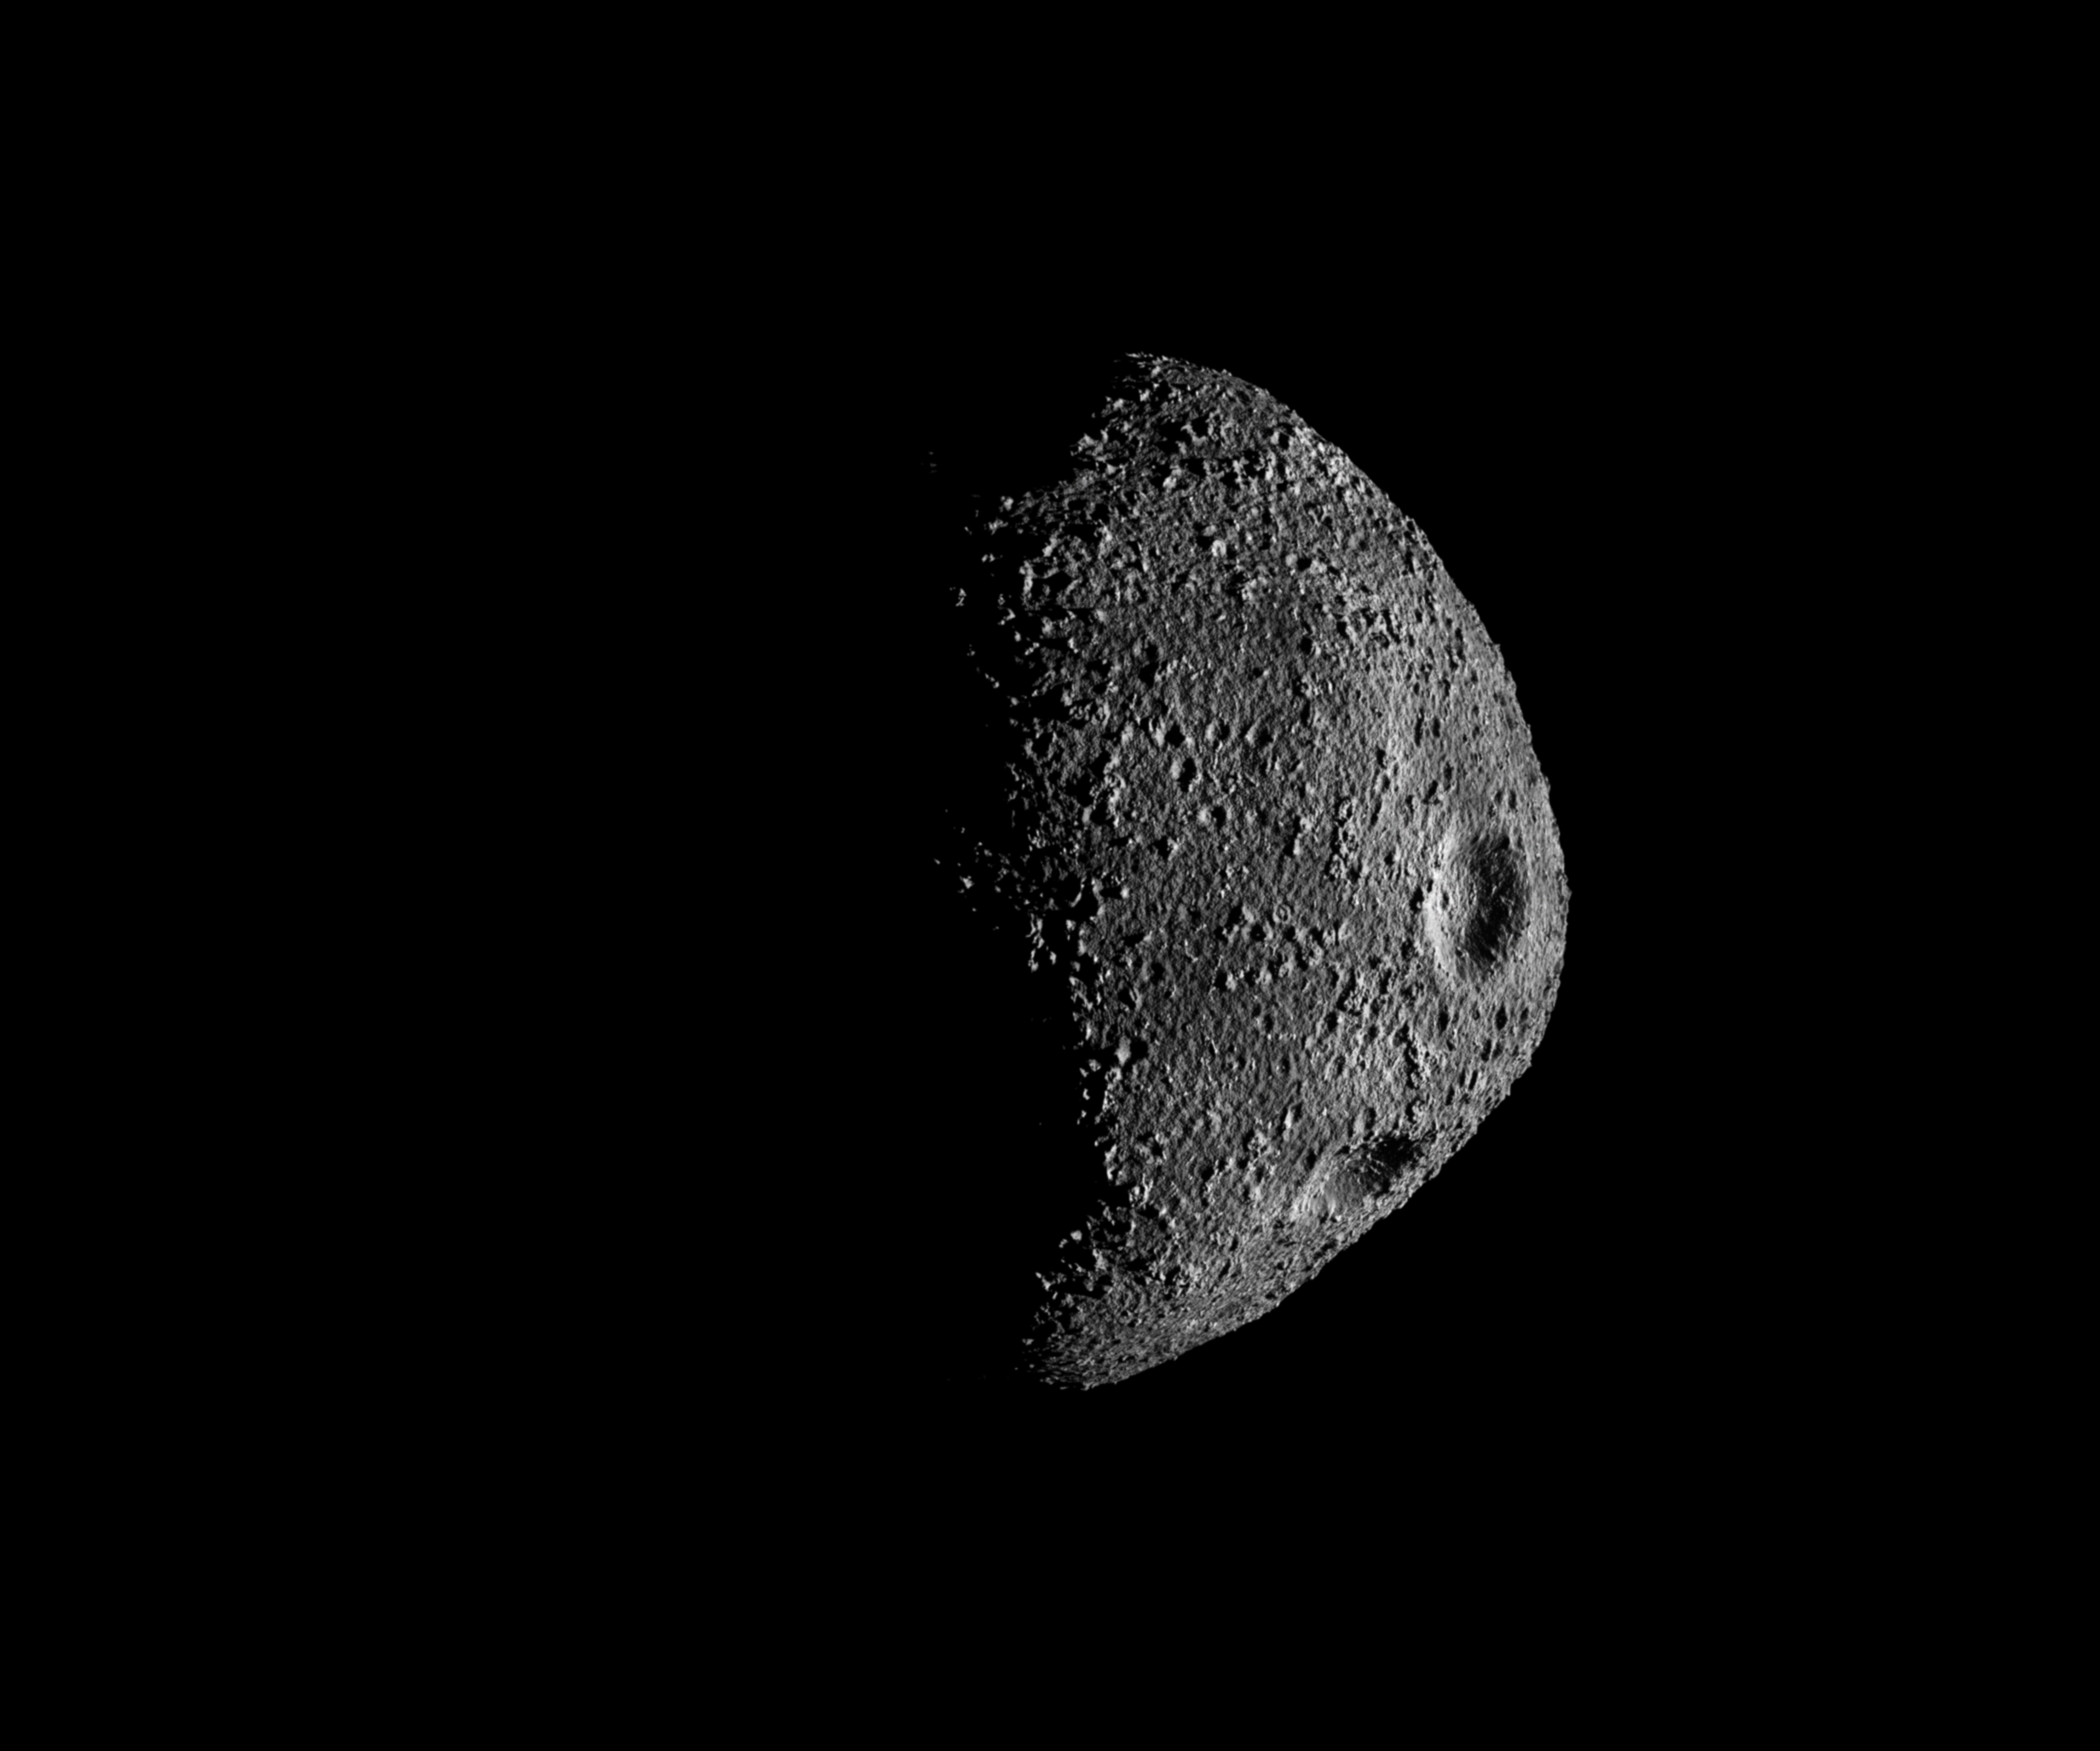
\includegraphics[width=\textwidth]{doc/thesis/0_figures/procedural_terrain/50_10_Inst_2017-08-15T115755-845000.png}
        \caption{}
        \label{fig:render_quali_comparison_1}
    \end{subfigure}
    \begin{subfigure}[b]{0.48\textwidth}
        \centering
        \includegraphics[width=\textwidth]{doc/thesis/0_figures/procedural_terrain/50_10_Inst_2017-08-15T115855-260000.png}
        \caption{}
        \label{fig:render_quali_comparison_2}
    \end{subfigure}
    \\
    \begin{subfigure}[b]{0.48\textwidth}
        \centering
        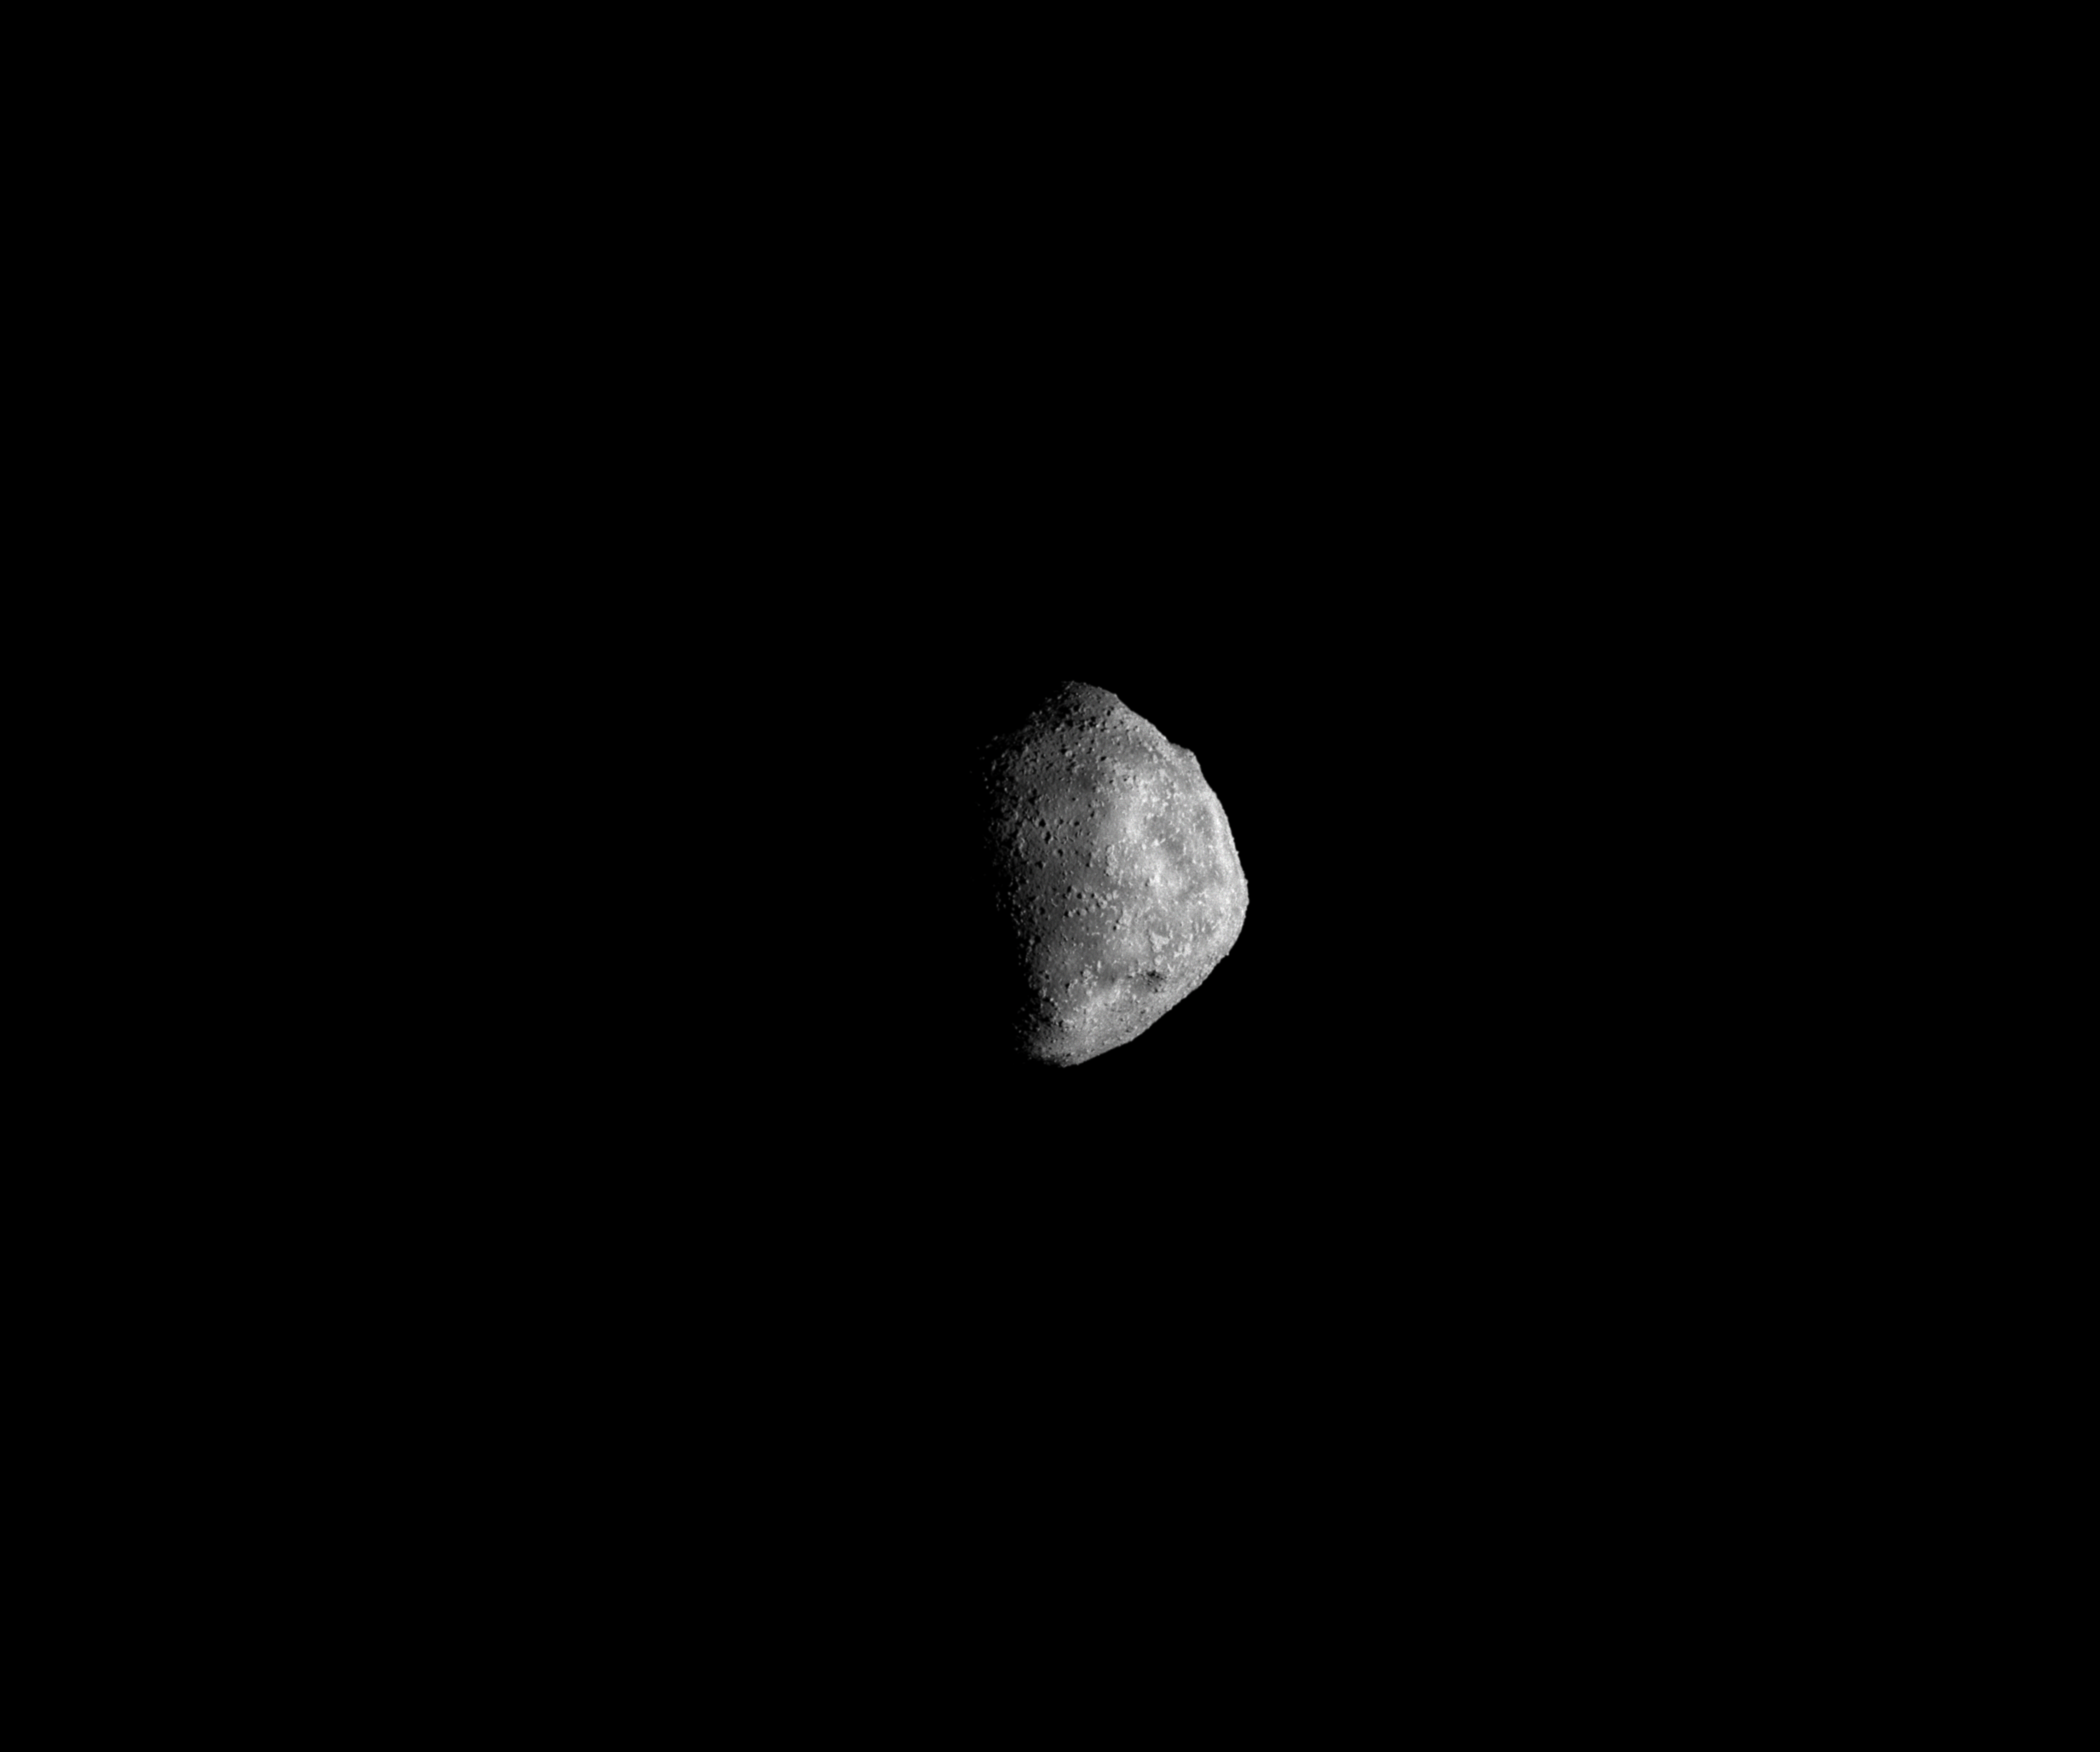
\includegraphics[width=\textwidth]{doc/thesis/0_figures/procedural_terrain/50_1_Inst_2017-08-15T115837-133000.png}
        \caption{}
        \label{fig:render_quali_comparison_3}
    \end{subfigure}
    \begin{subfigure}[b]{0.48\textwidth}
        \centering
        \includegraphics[width=\textwidth]{doc/thesis/0_figures/procedural_terrain/50_1_Inst_2017-08-15T115851-232000.png}
        \caption{}
        \label{fig:render_quali_comparison_4}
    \end{subfigure}
    \caption{Rendered images of differently sized \glspl{sssb} from varying distances. (a)~Nucleus of \SI{10}{\kilo\meter} from \SI{566}{\kilo\meter} distance. (b)~Nucleus of \SI{10}{\kilo\meter} from \SI{106}{\kilo\meter} distance. (c)~Nucleus of \SI{1}{\kilo\meter} from \SI{149}{\kilo\meter} distance. (d)~Nucleus of \SI{1}{\kilo\meter} from \SI{50}{\kilo\meter} distance.}
    \label{fig:render_quali_comparison}
\end{figure}

\begin{figure}[htb]
    \centering
    \begin{subfigure}[b]{\textwidth}
        \centering
        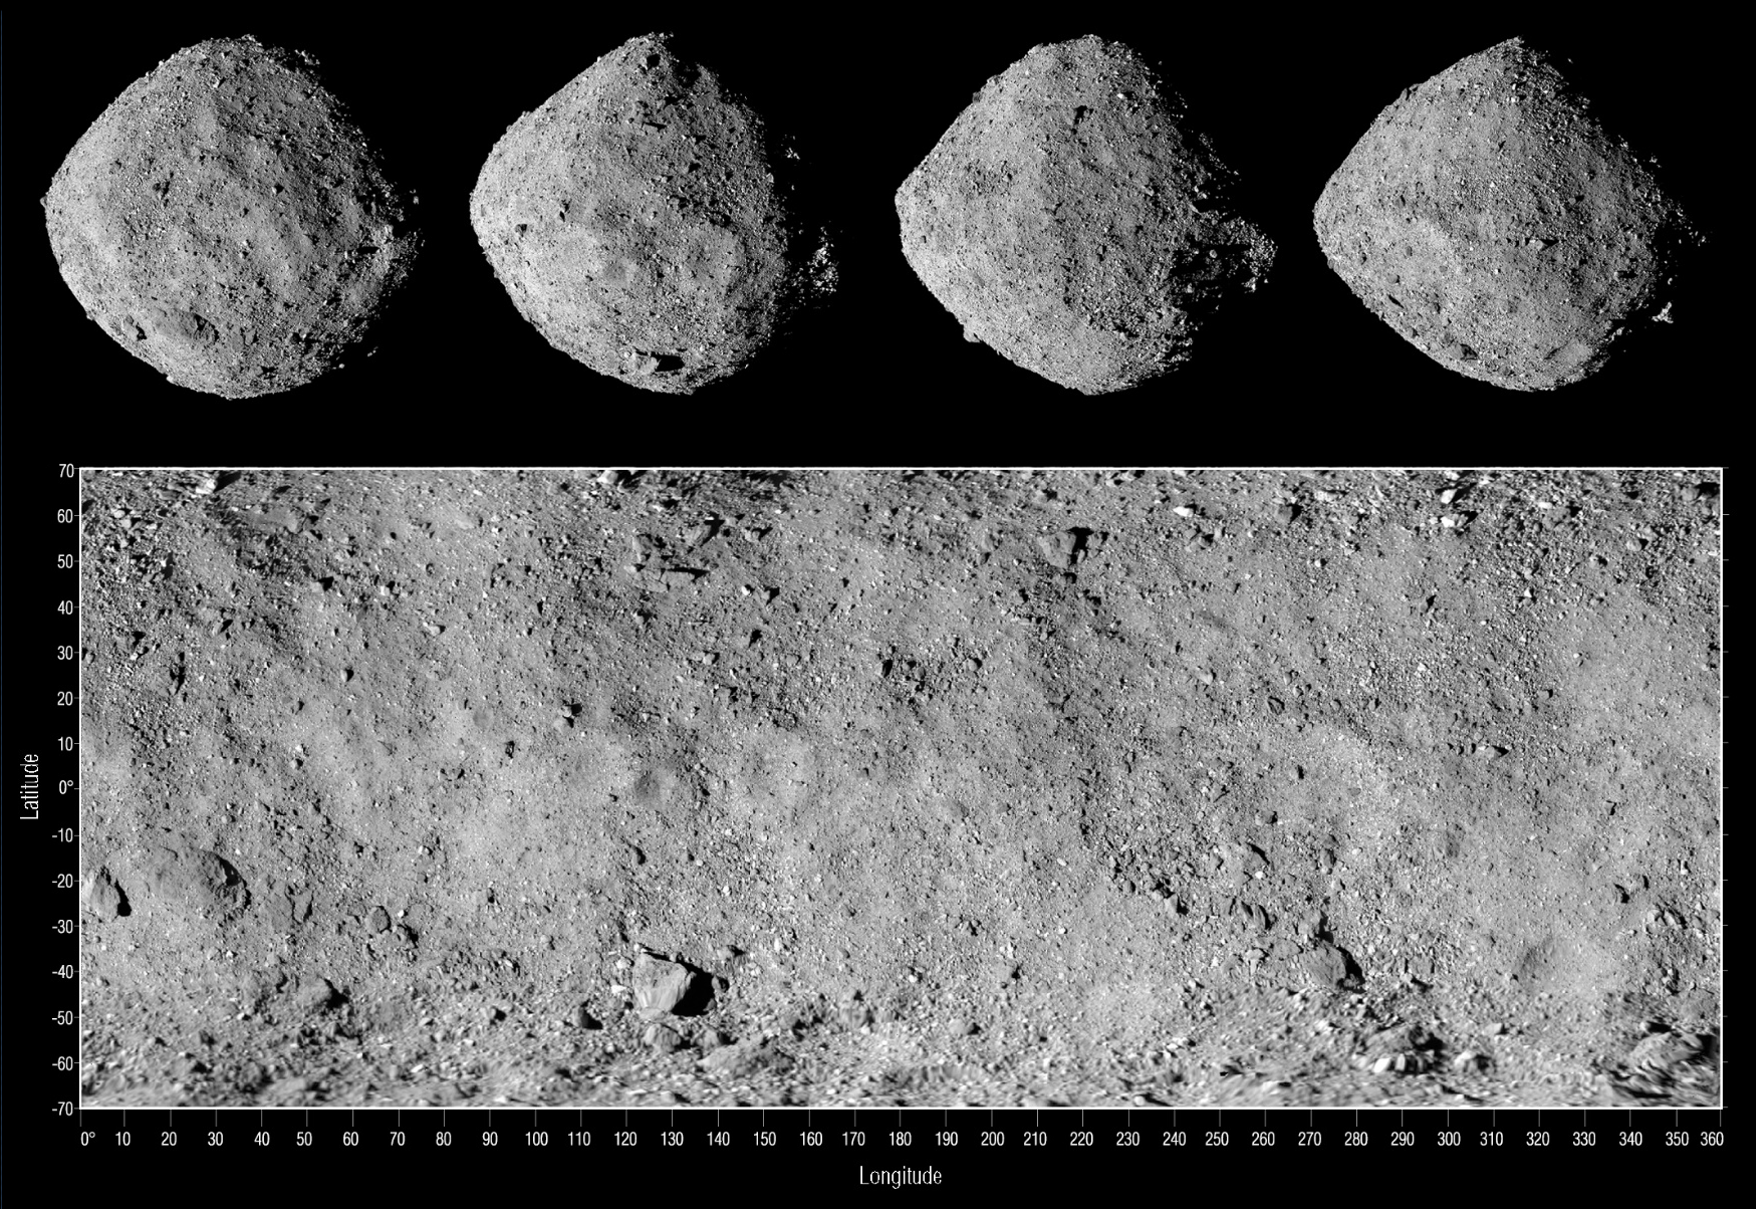
\includegraphics[width=\textwidth]{doc/thesis/0_figures/procedural_terrain/2963_Bennu.png}
        \caption{}
        \label{fig:render_quali_bennu}
    \end{subfigure}
    \\
    \begin{subfigure}[b]{0.425\textwidth}
        \centering
        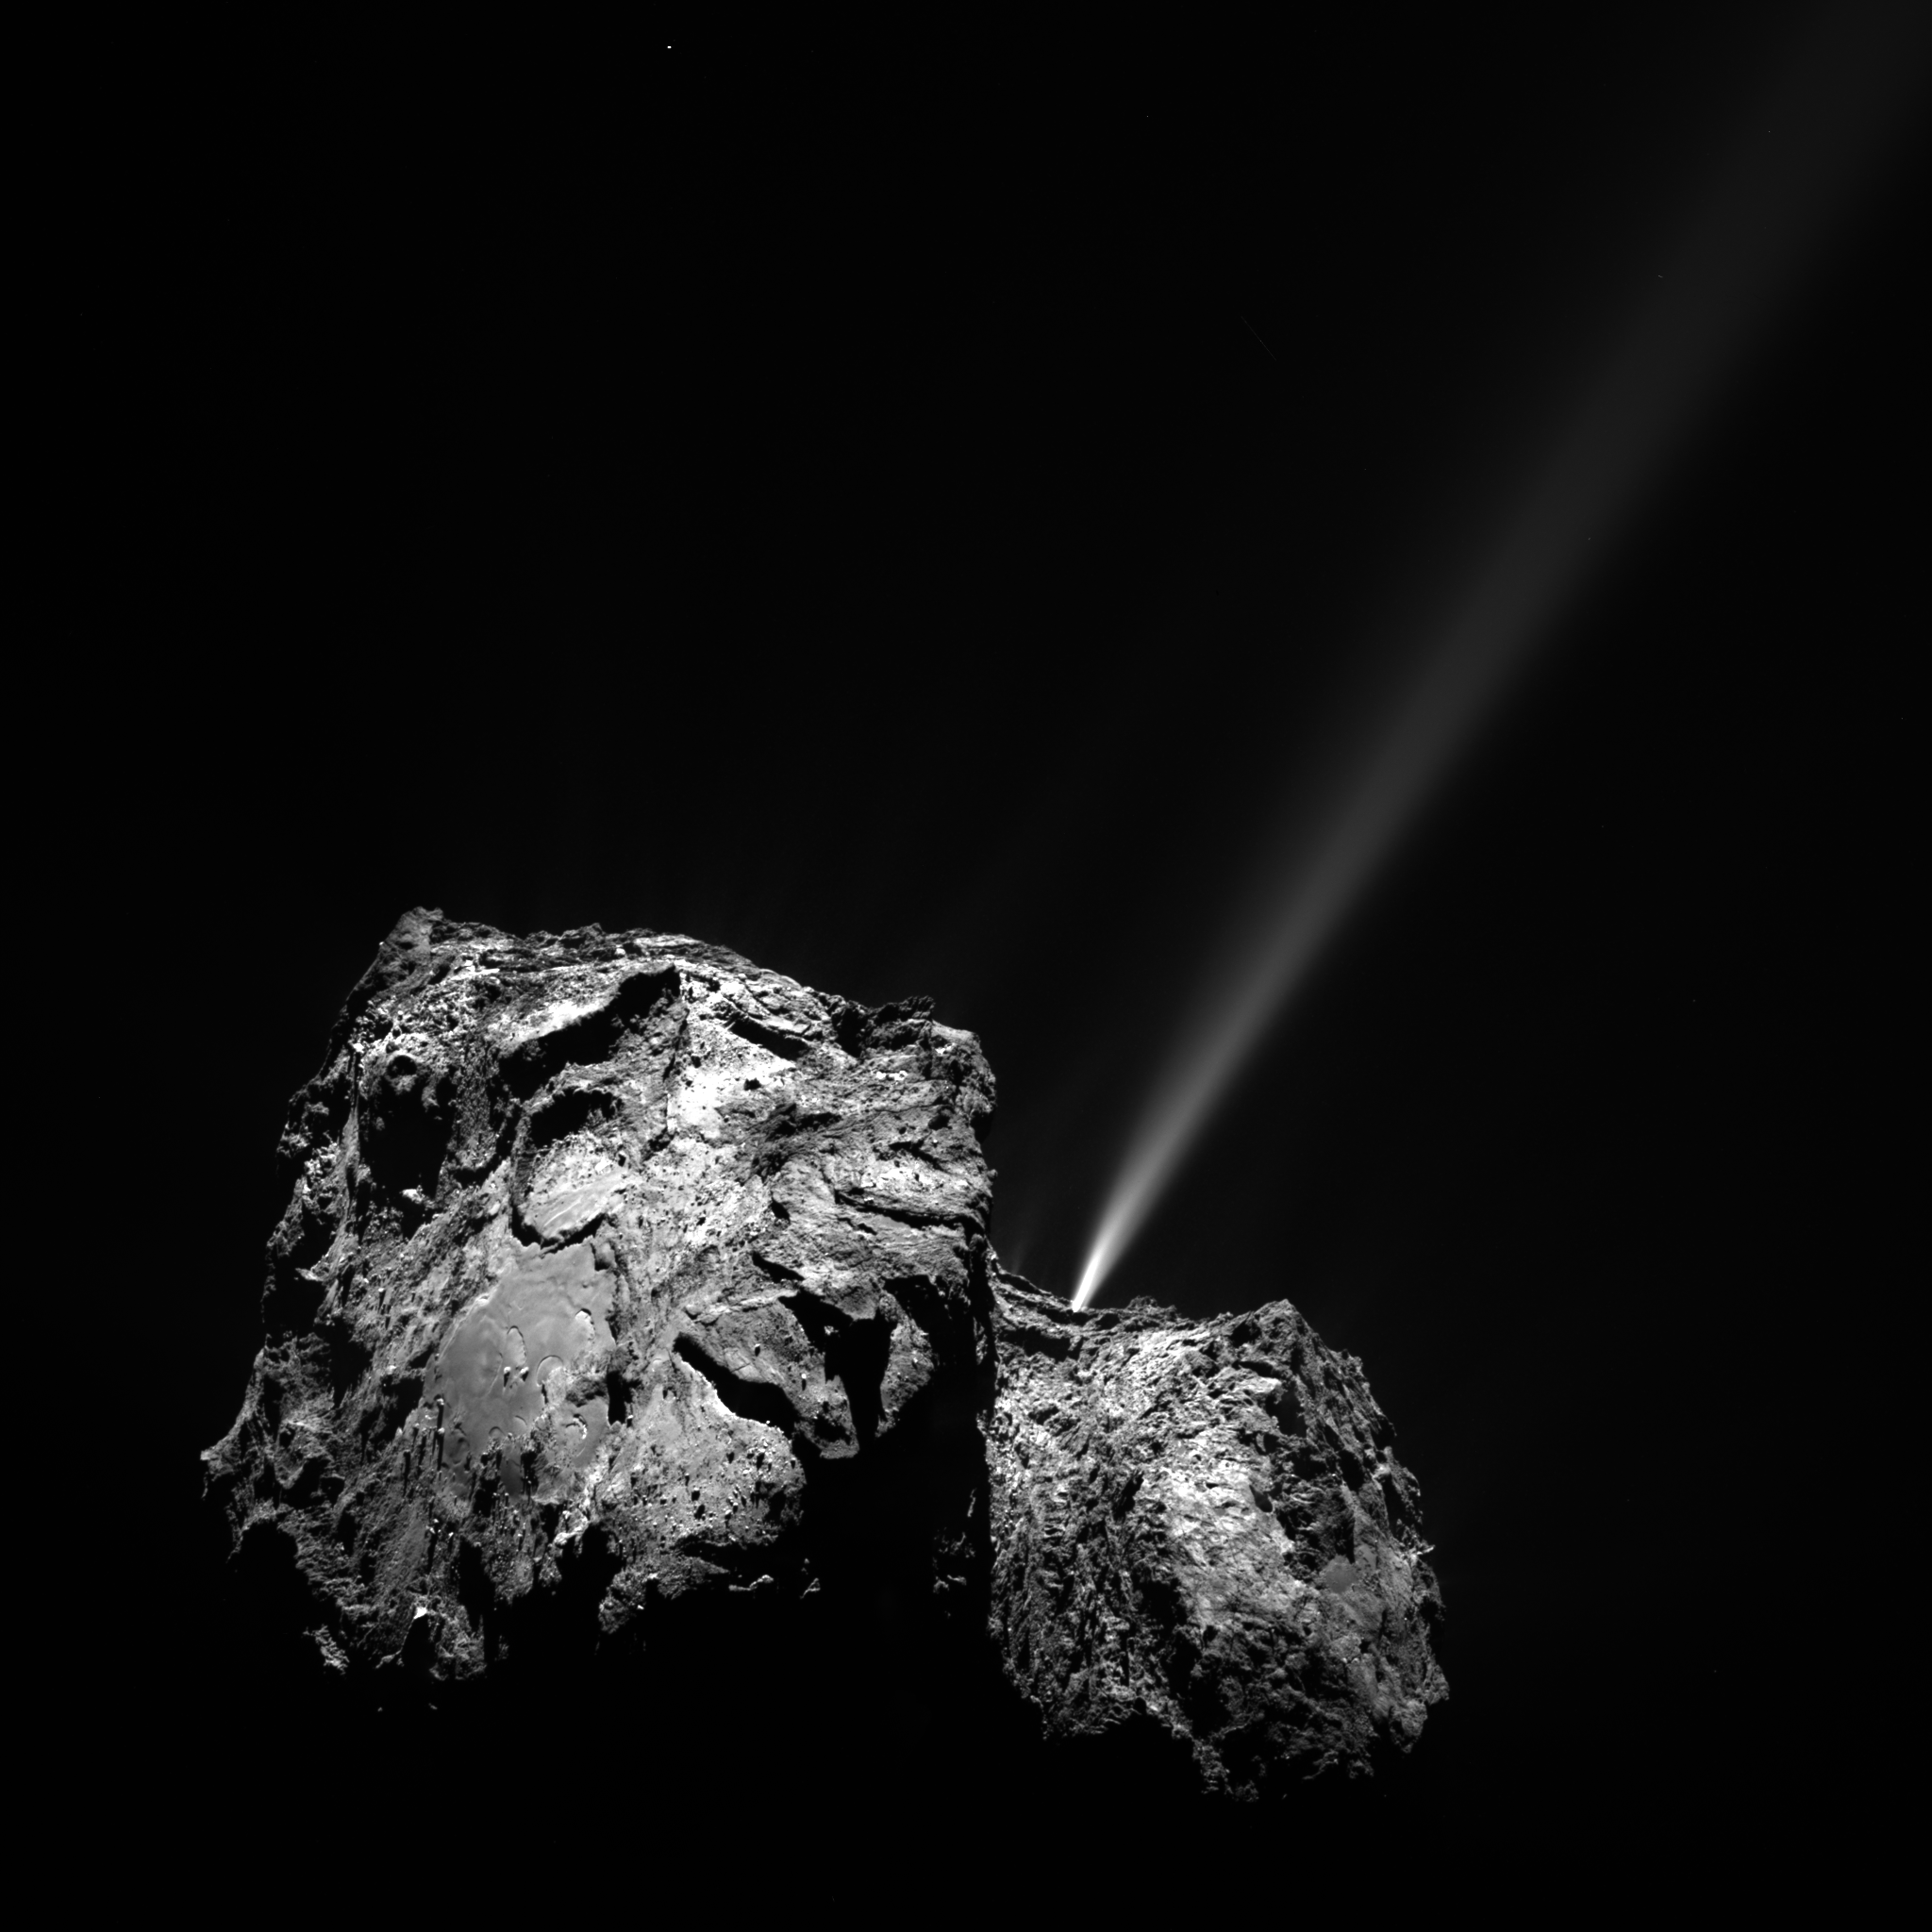
\includegraphics[width=\textwidth]{doc/thesis/0_figures/procedural_terrain/67P_CG.PNG}
        \caption{}
        \label{fig:render_quali_67p}
    \end{subfigure} %
    \begin{subfigure}[b]{0.565\textwidth}
        \centering
        \includegraphics[height=\textwidth, angle=90]{doc/thesis/0_figures/procedural_terrain/Wild2.jpg}
        \caption{}
        \label{fig:render_quali_81p}
    \end{subfigure}
    \caption{(a)~Four images of asteroid Bennu and a global surface mosaic. The images were taken by the PolyCam aboard the \textit{OSIRIS-REx} mission~\cite{NASAFourBennu}. (b)~Representative image of comet \gls{67p}. The image was captured by the OSIRIS imager aboard the \textit{Rosetta} mission~\cite{OSIRISArchiveb}. (c)~Image collection of comet \gls{81p} taken during the \textit{Stardust} mission by its navigation camera~\cite{StardustImages}.}
    \label{fig:render_quali}
\end{figure}

All objects in Figures~\ref{fig:render_quali_comparison}~and~\ref{fig:render_quali} show pits. The overall appearance of the rendered images resembles the smoother pits of Bennu better than the sharper pits of \gls{67p} or \gls{81p}. The rocks and boulders on Bennu's surface appear similar to the rocks and boulders in the rendered images, especially Figures~\ref{fig:render_quali_comparison_1}~and~\ref{fig:render_quali_comparison_2}. The most pronounced difference between rendered images and the images of \gls{67p} or \gls{81p} are jets. \Gls{sispo} does not yet contain a gas and dust model that would produce a coma or jets. Therefore, coma and jets are missing in the rendered images. While the surface of both comets feature some boulders, their surfaces are more defined by ridge-like structures. Ridge-like features are missing in the rendered images. Consequently, the rendering images of \gls{sispo} are more similar to asteroids than comets.

Procedural terrain generation within \gls{sispo} creates results for a large range of encounter distances. Images with different surface distances and \gls{sssb} sizes are presented in Figure~\ref{fig:render_quali_comparison}. No visual degradation of surface features and details is visible in Figure~\ref{fig:render_quali_comparison}. Moving closer to the surface reveals more details, such as tiny bumps between larger structures which are not visible from larger distances. The visible quality of surface features is defined by the shader implementation. 

\clearpage

\subsubsection{Image Composition}
The composition process uses raw images rendered with Blender and produces photometrically calibrated images. An example set of four images consisting of two images before and after calibration is shown in Figure~\ref{fig:composition_before_after}. Two effects can be seen. First, the overall brightness differs in the original images. The brightness difference is corrected by calibration in the processed images. Secondly, images become brighter by the composition process. Image brightening originates from scaling images to the interval $[0,1]$.

\begin{figure}[htb]
    \centering
    \begin{subfigure}[b]{\textwidth}
        \centering
        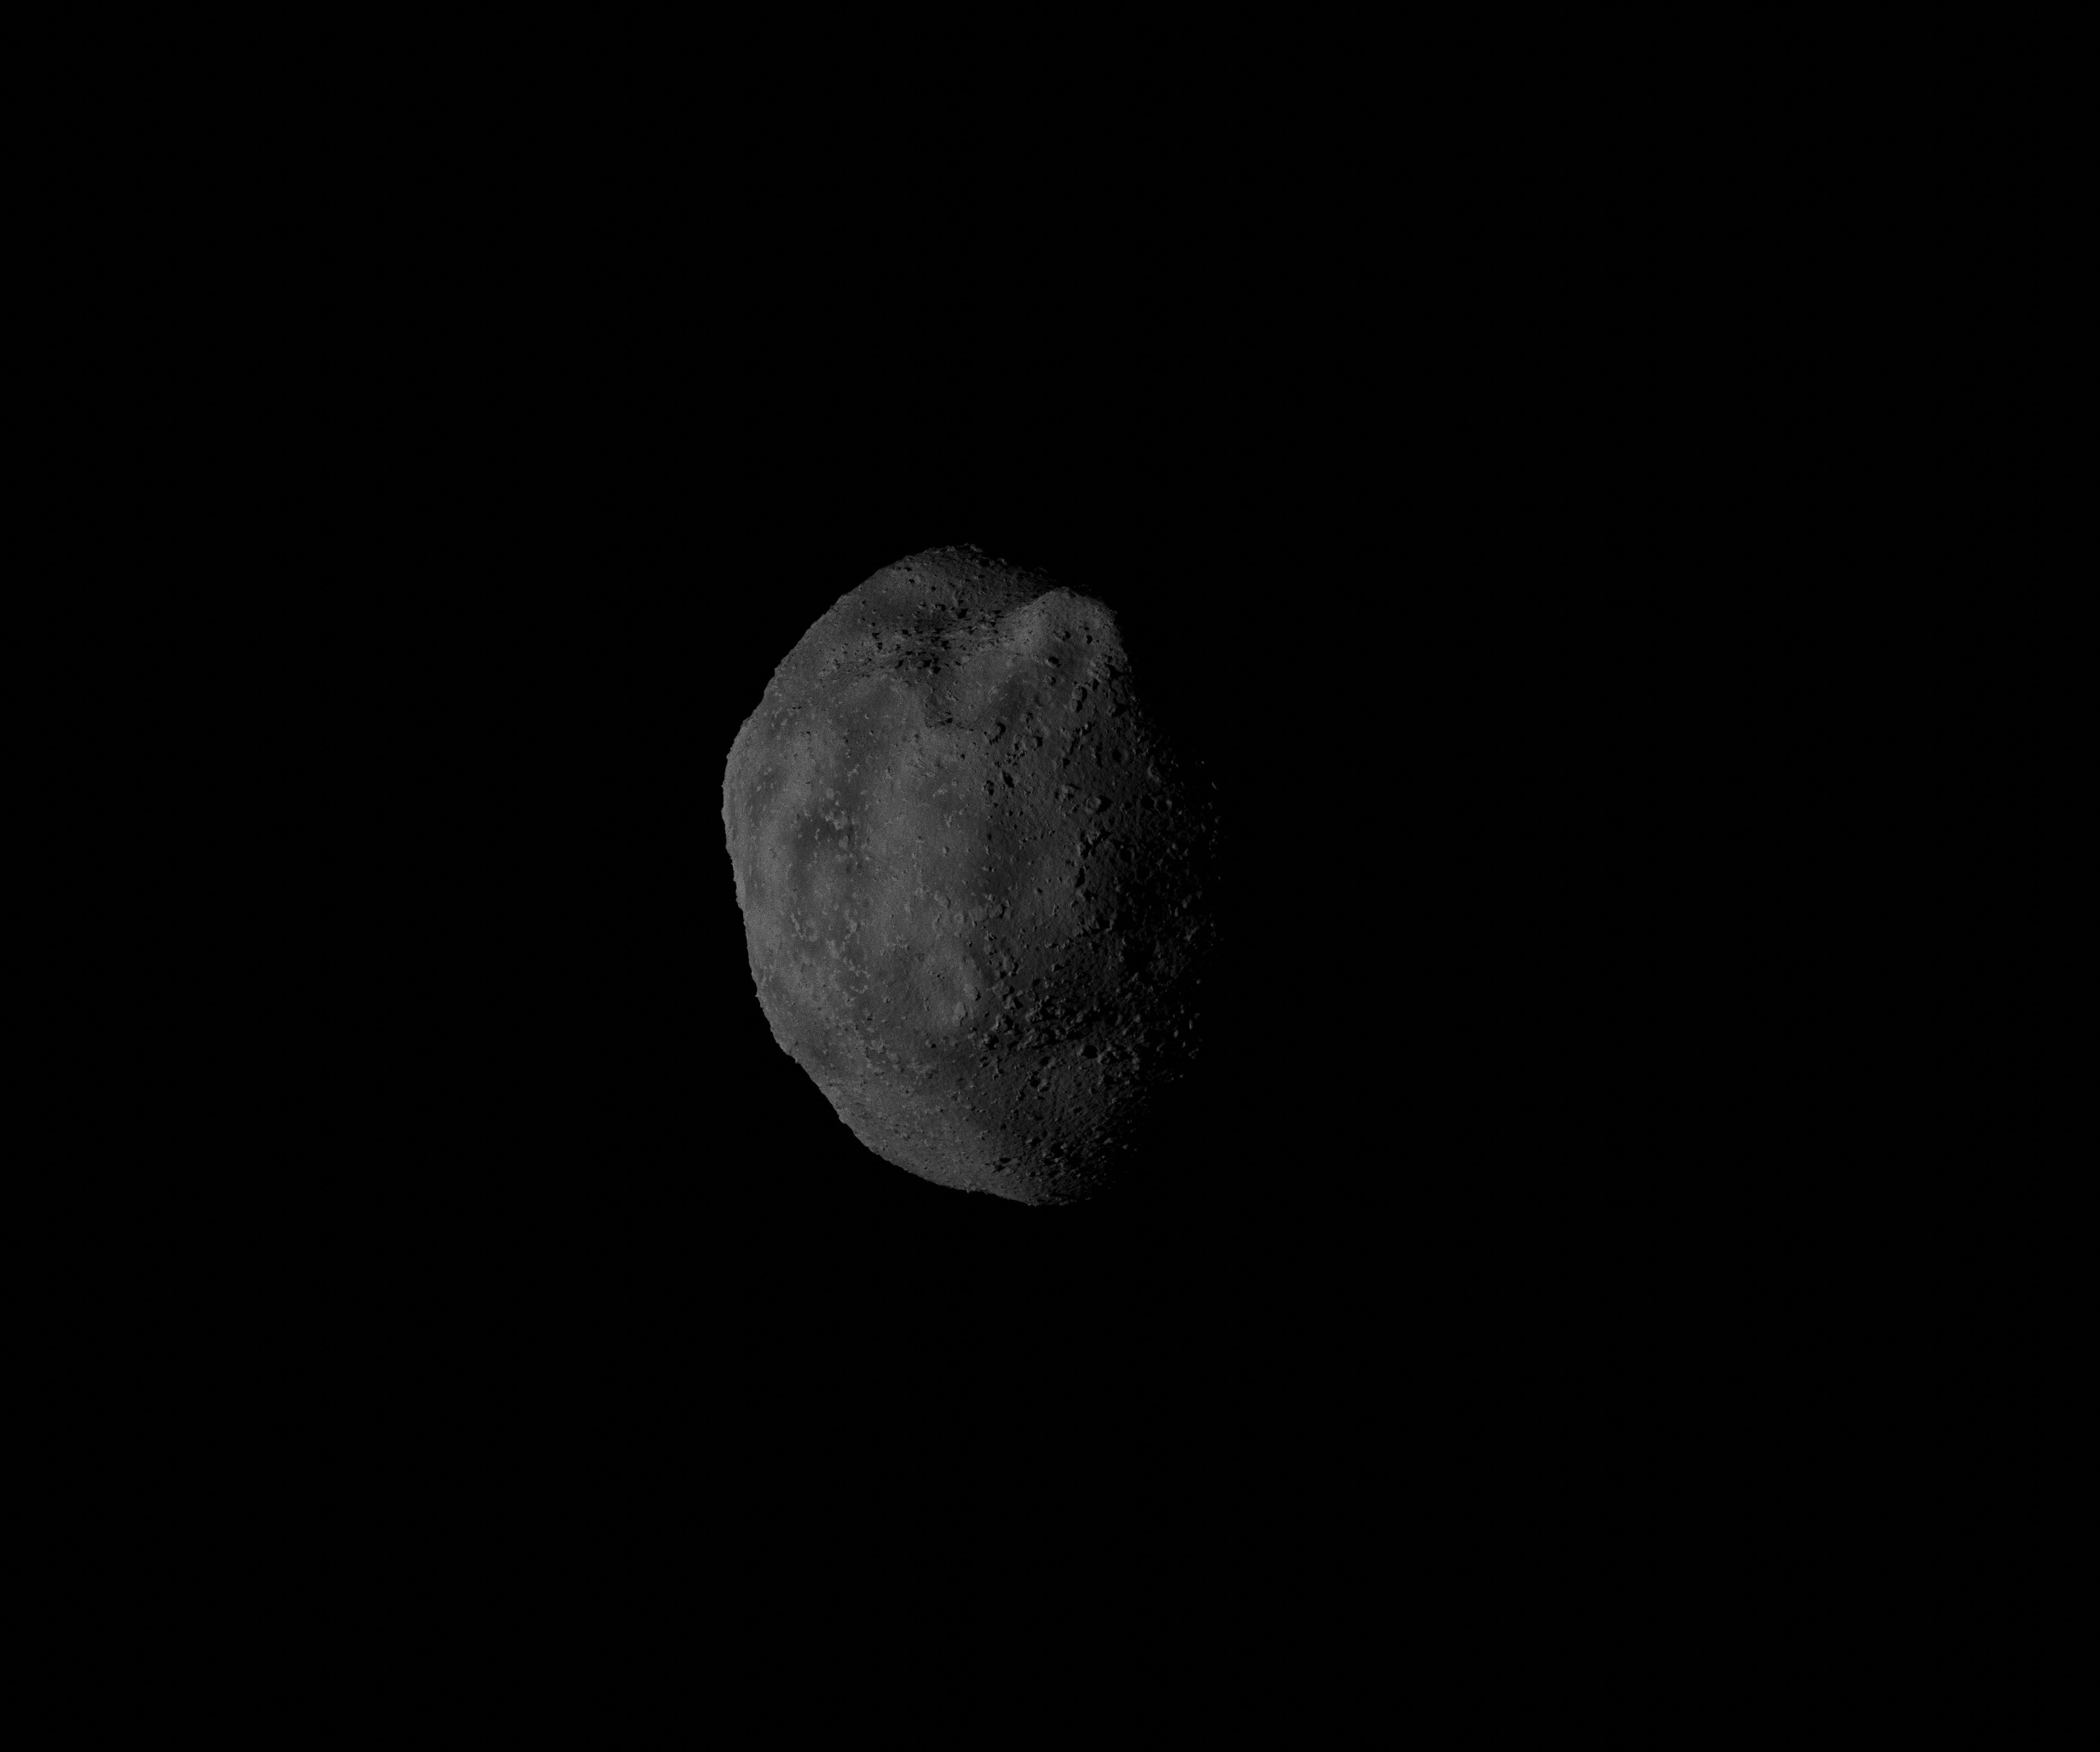
\includegraphics[width=0.49\textwidth]{doc/thesis/0_figures/rendering_lighting/SssbOnly_2017-08-15T115858-281000.jpg}
        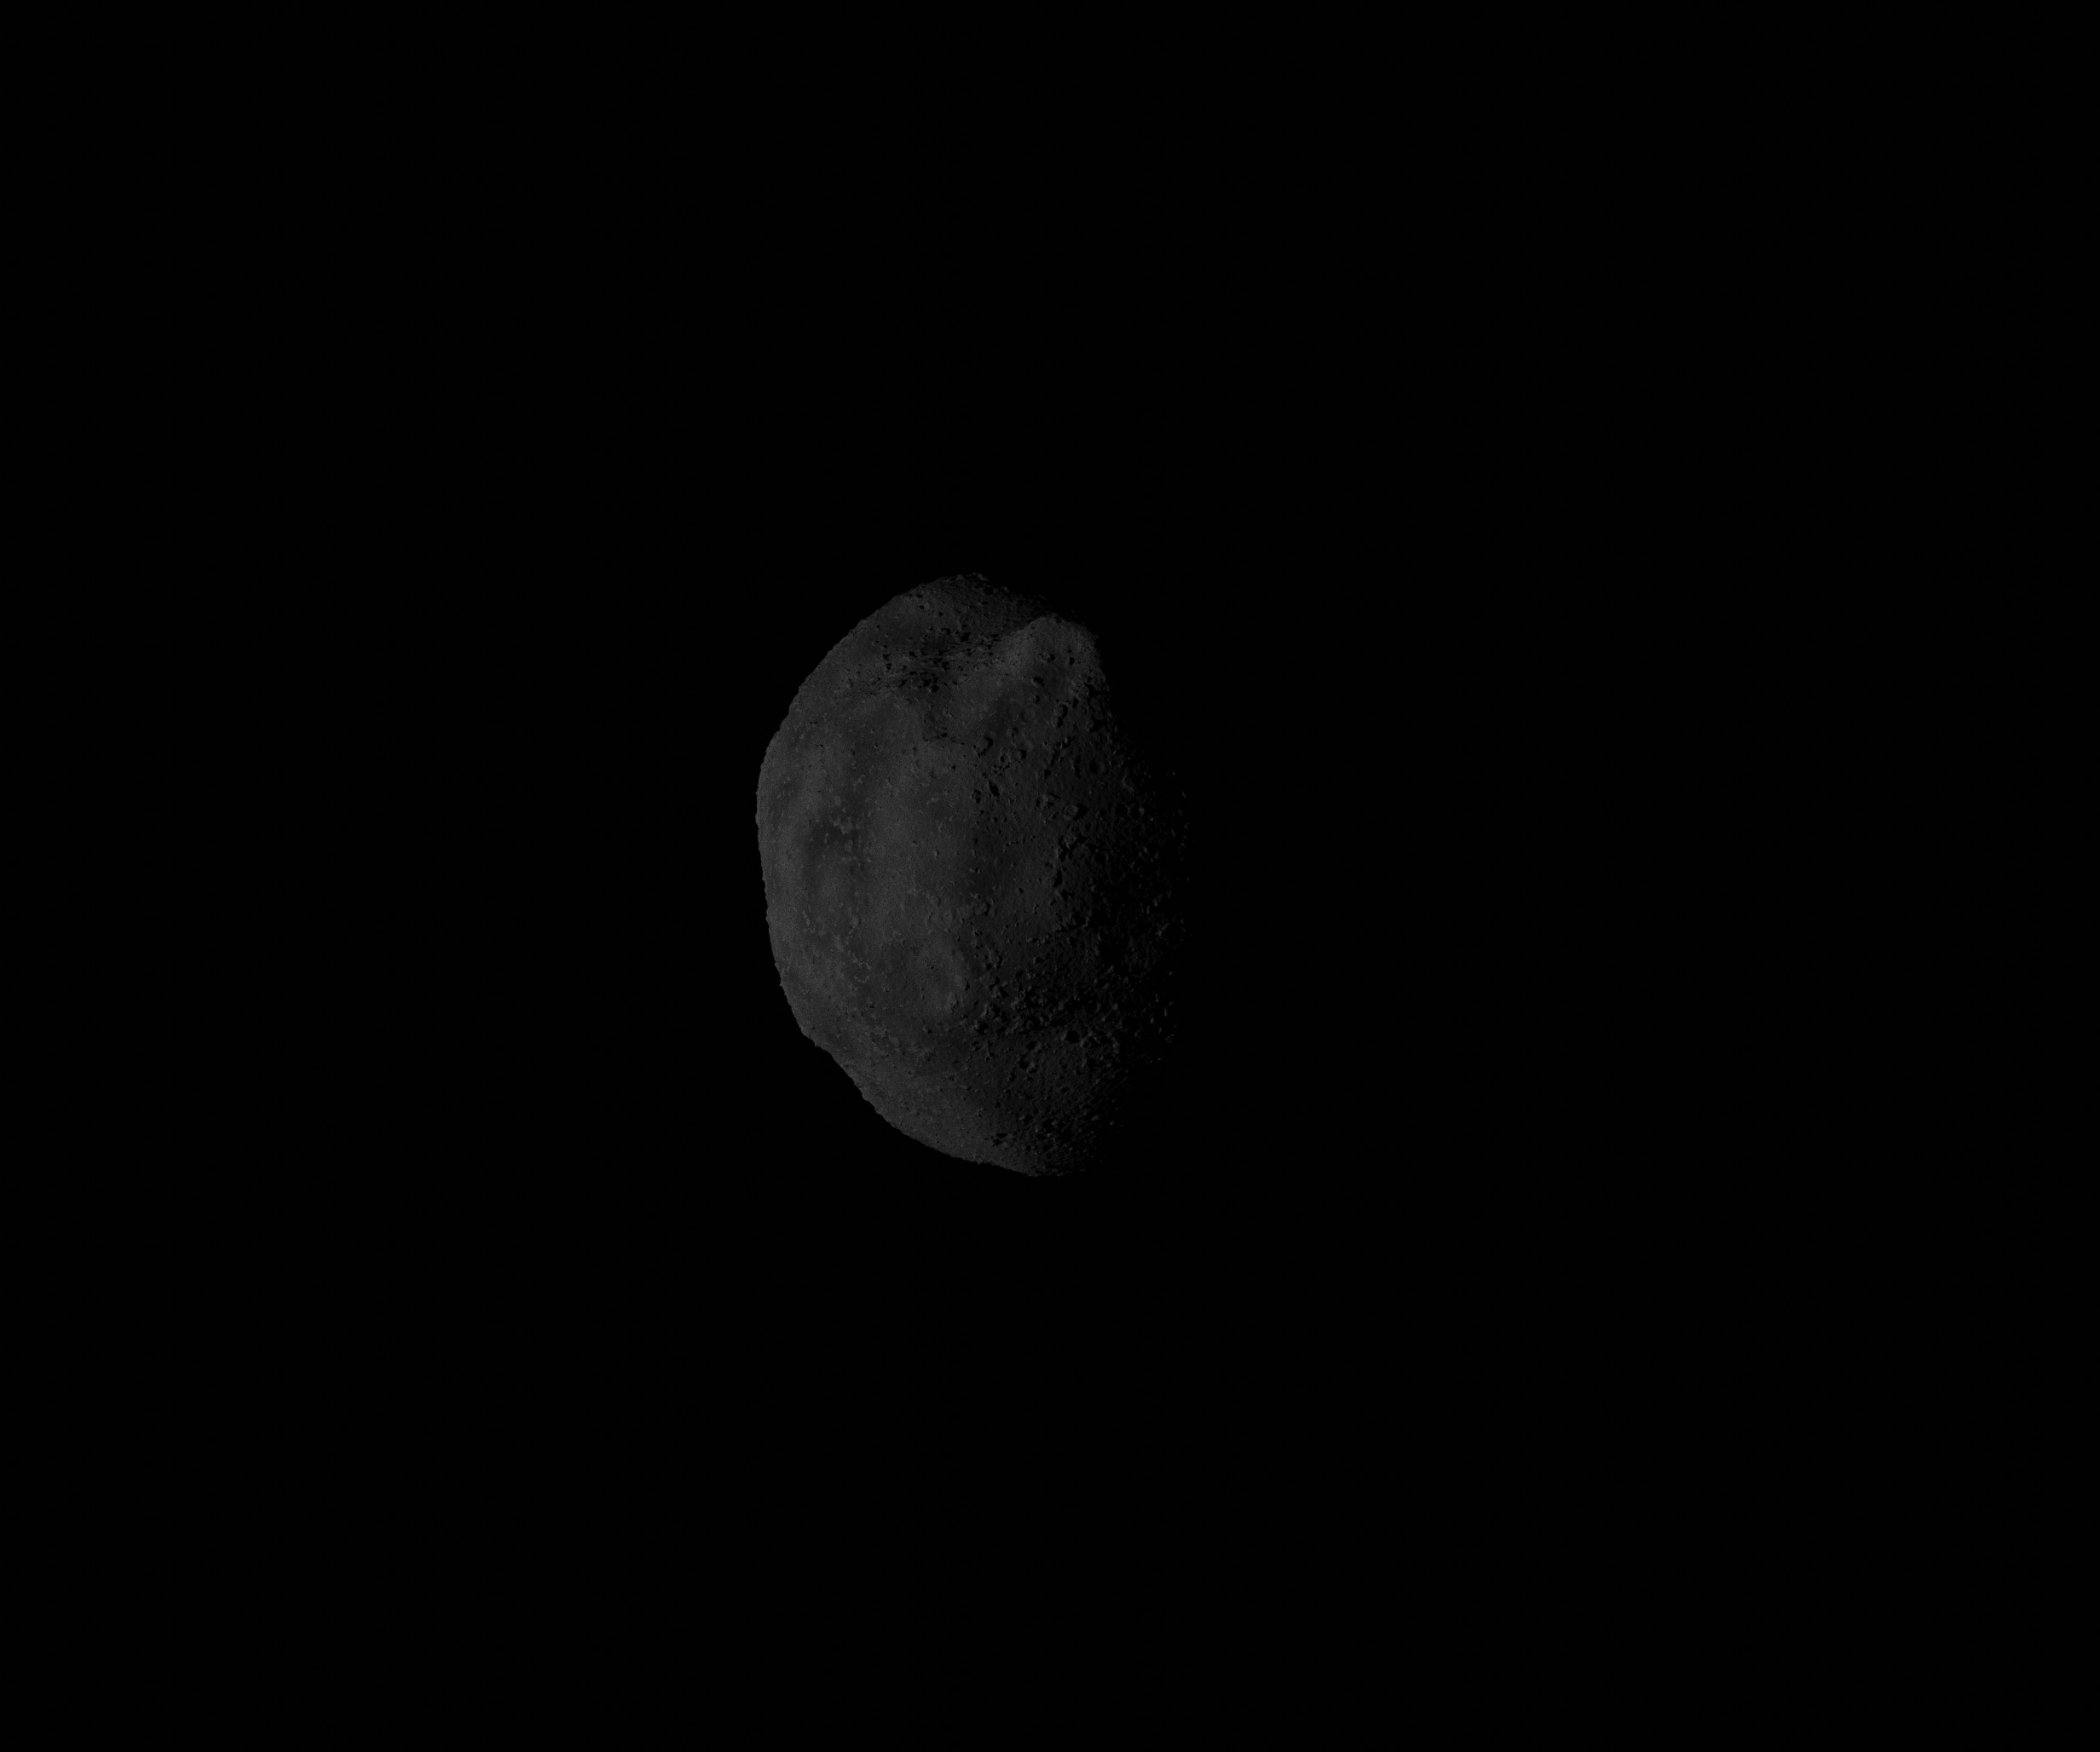
\includegraphics[width=0.49\textwidth]{doc/thesis/0_figures/rendering_lighting/SssbOnly_2017-08-15T115859-288000.jpg}
        % \caption{}
        % \label{fig:composition_before_1}
    \end{subfigure}
    \\
    \begin{subfigure}[b]{\textwidth}
        \centering
        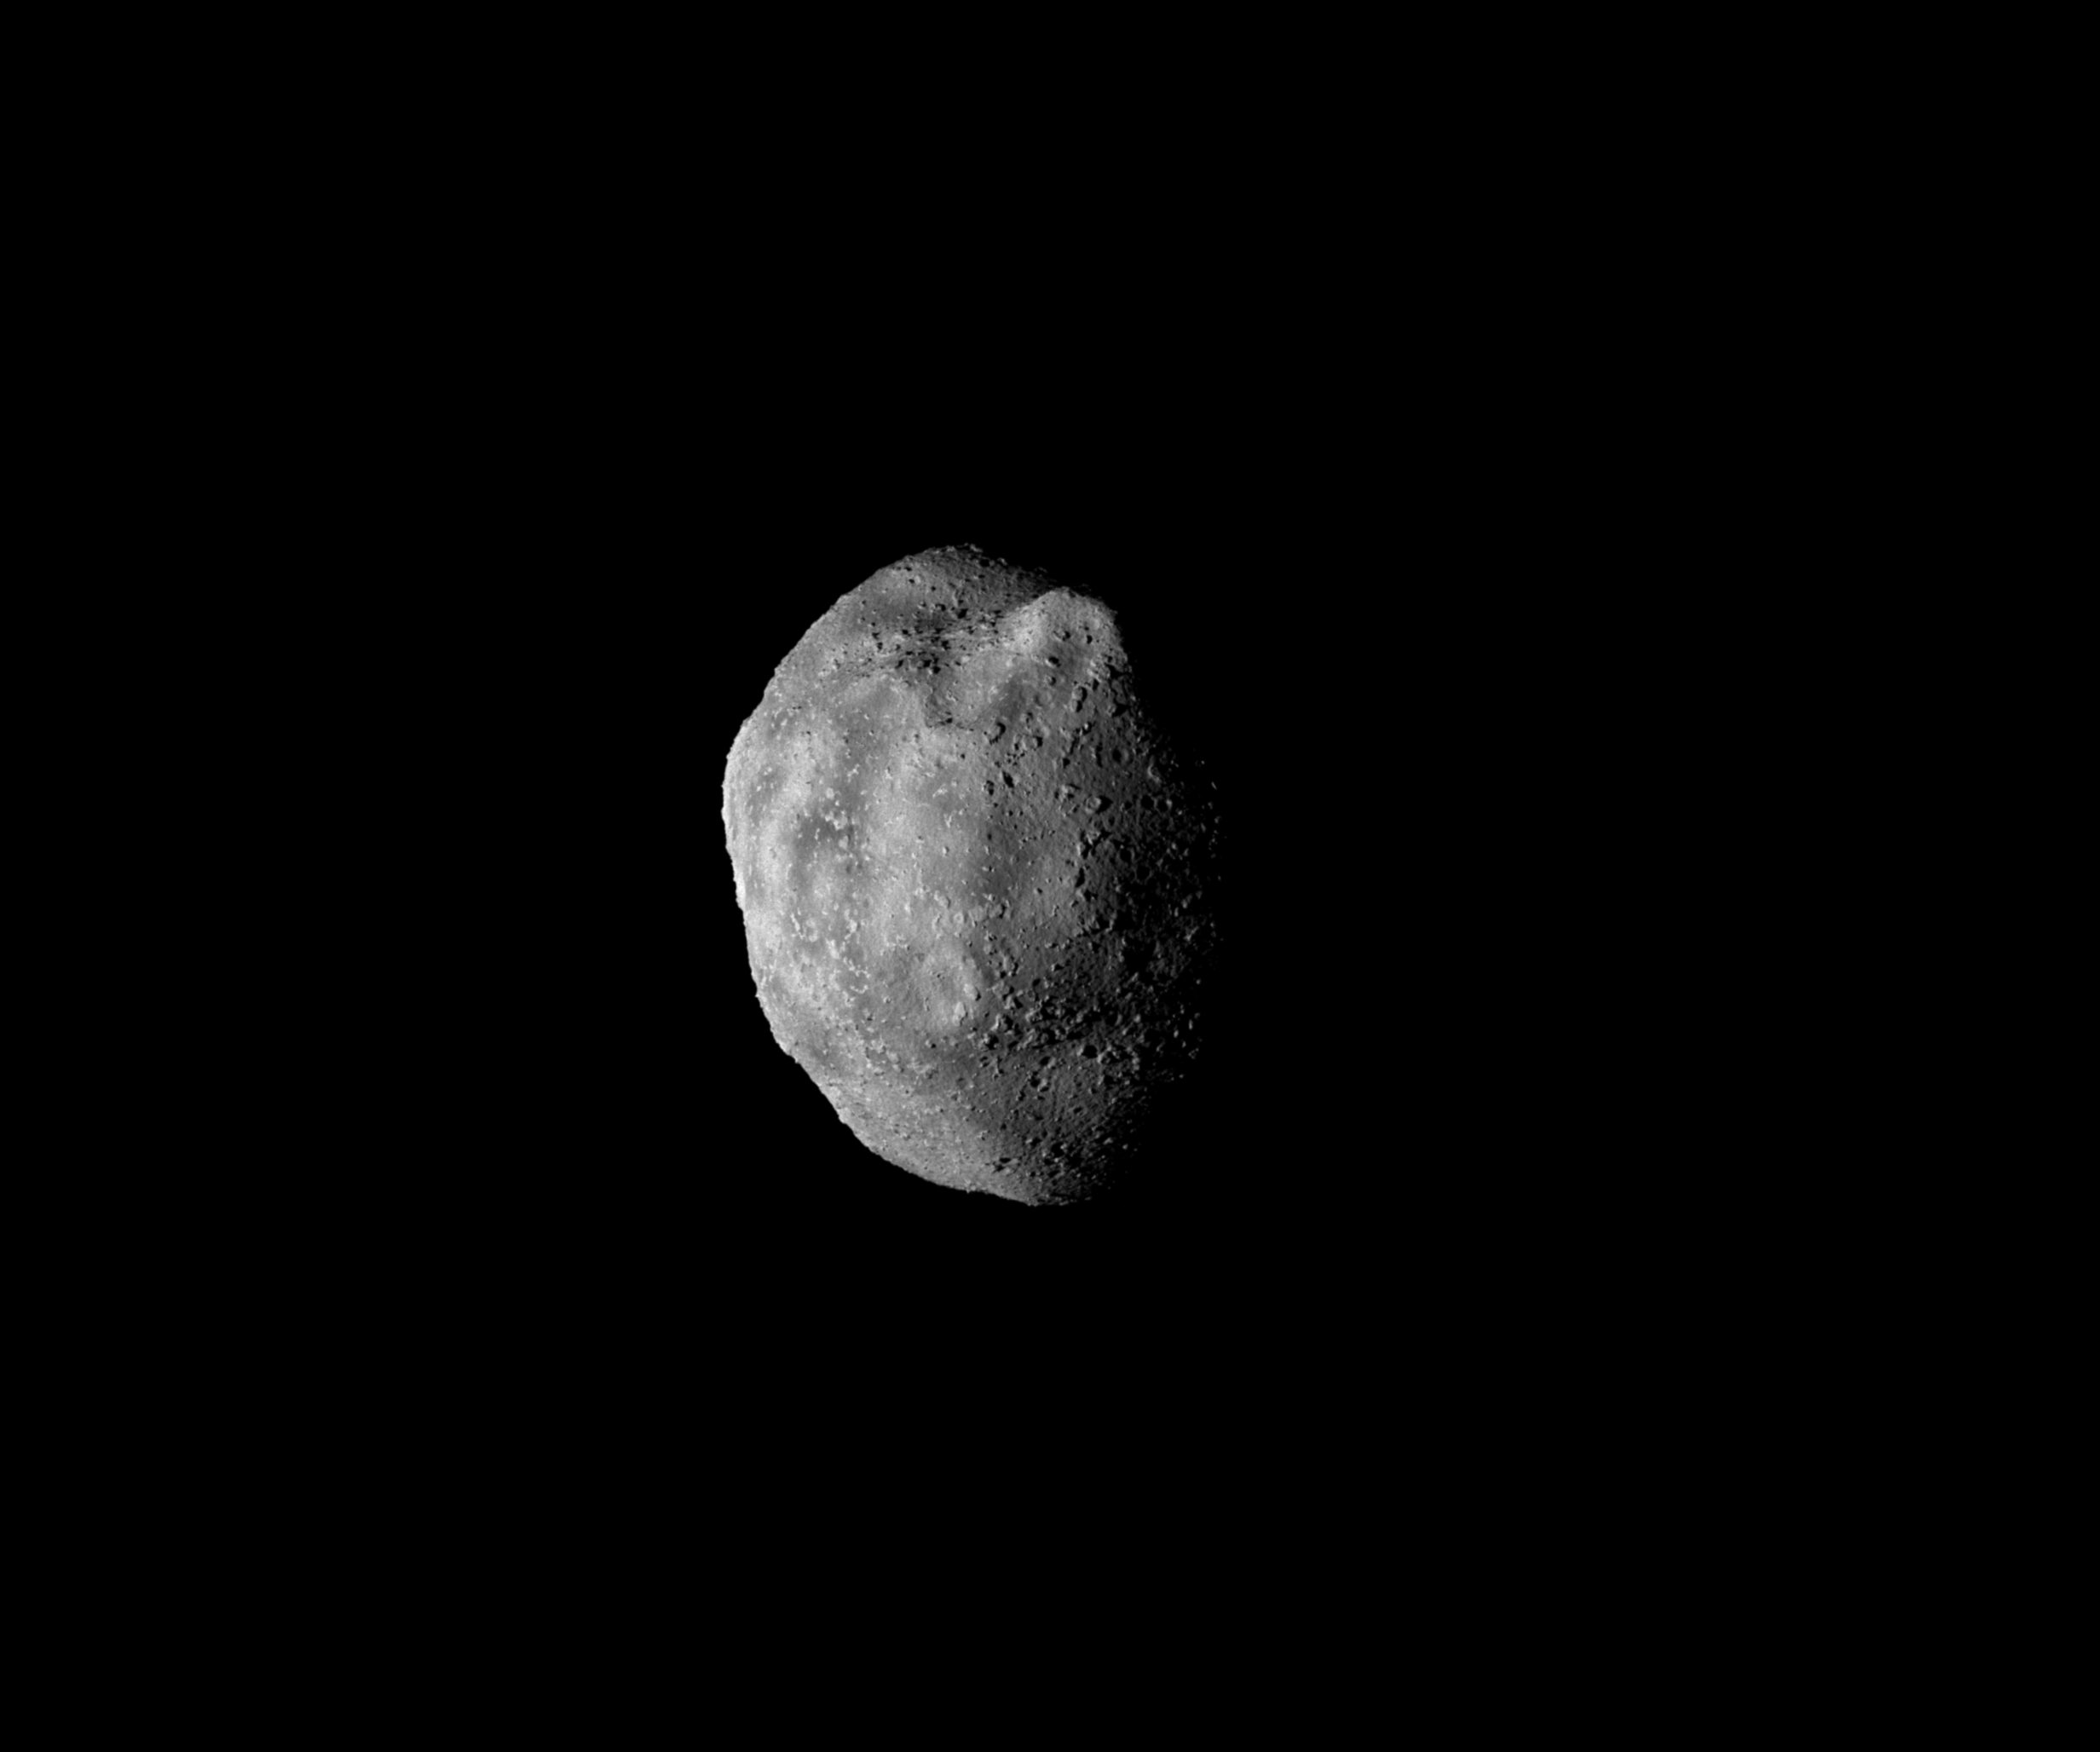
\includegraphics[width=0.49\textwidth]{doc/thesis/0_figures/rendering_lighting/Inst_2017-08-15T115858-281000.png}
        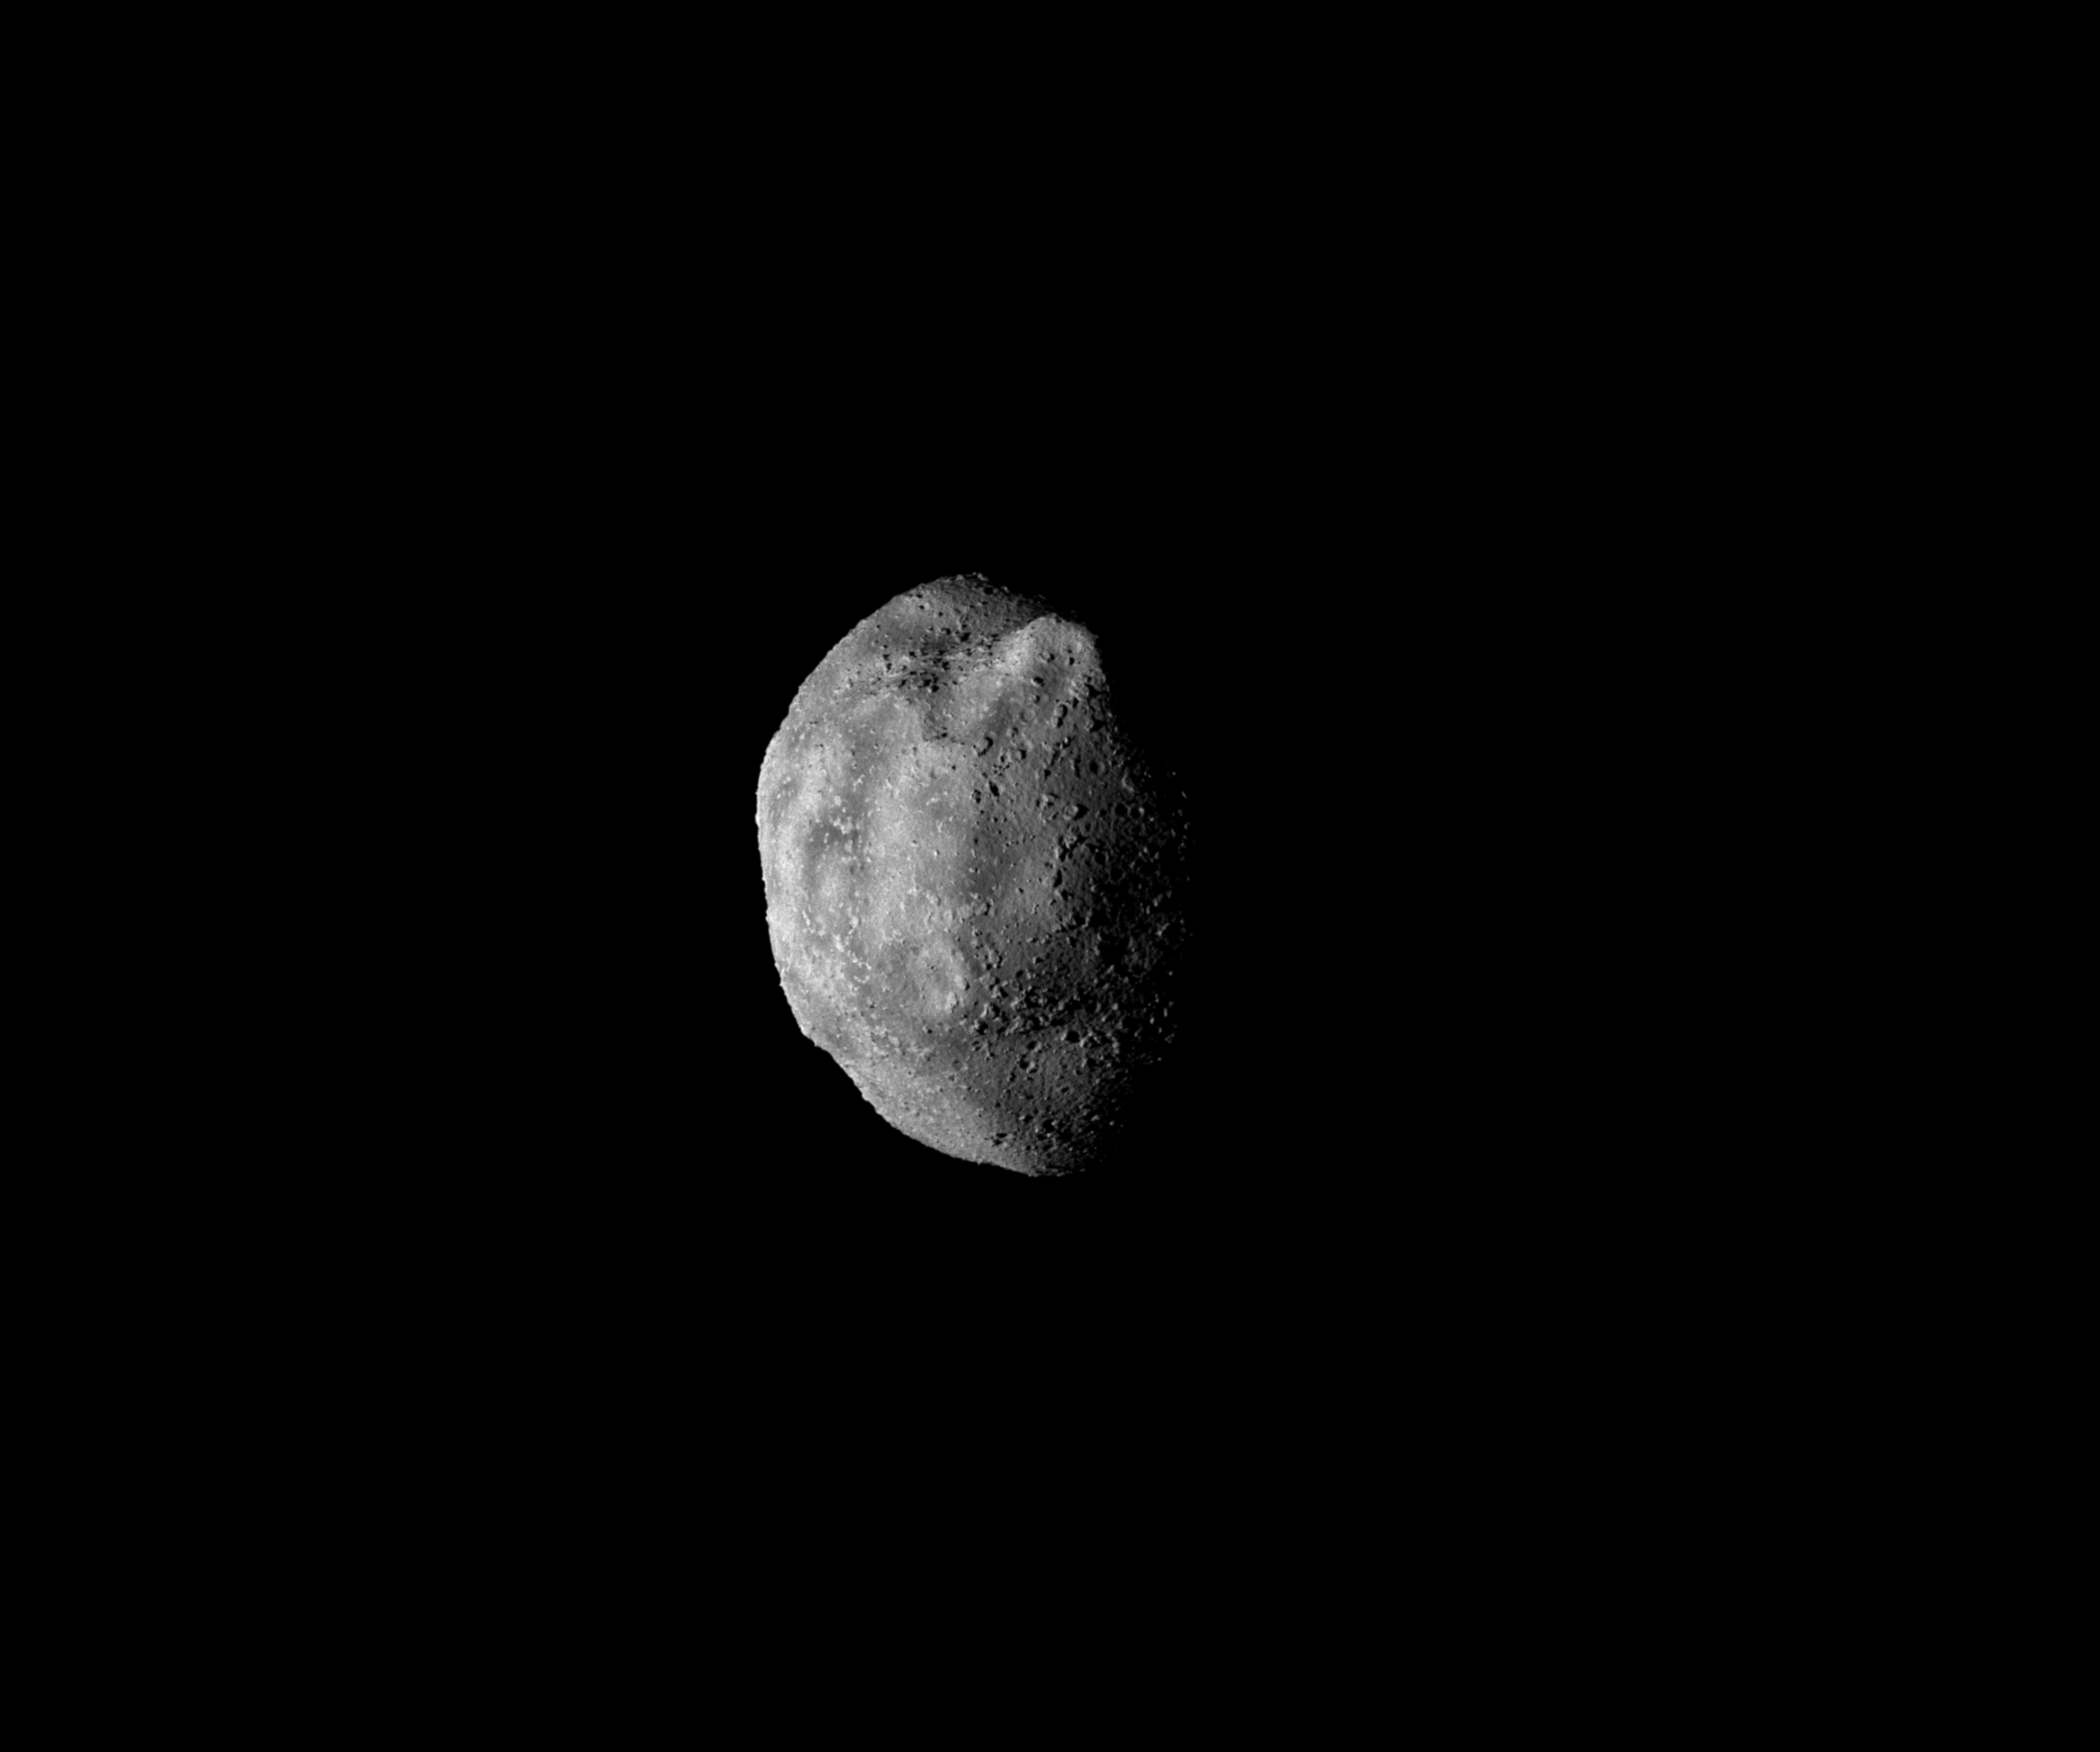
\includegraphics[width=0.49\textwidth]{doc/thesis/0_figures/rendering_lighting/Inst_2017-08-15T115859-288000.png}
        % \caption{}
        % \label{fig:composition_after_1}
    \end{subfigure}
    \caption{Two consecutive images before (top) and after (bottom) composition and calibration. The nucleus is much brighter than background stars thus no stars are visible in these images after calibration. The four images are reduced to \SI{8}{\bit} colour depth.}
    \label{fig:composition_before_after}
\end{figure}

\subsubsection{Rendering Problems} \label{sec:render_problems}
Rendered images of a fly-by scenario with a \SI{10}{\kilo\meter} \gls{sssb} contain artefacts. Figure~\ref{fig:render_artefacts} shows rendered images of fly-bys with varying fly-by distances. All three images are raw rendered images, before composition. The images show a stripe, a darker patch across the \gls{sssb} with sharp brightness transitions. The stripe is at the same location across the nucleus in all three images. The stripe artefact does not appear in all images with a \SI{10}{\kilo\meter} \gls{sssb} and not for other \gls{sssb} sizes. The most likely explanation are errors while scaling the nucleus from the original \SI{1}{\kilo\meter} to the \SI{10}{\kilo\meter} model issues with the shader implementation.
\begin{figure}[htb]
    \centering
    \begin{subfigure}[b]{0.32\textwidth}
        \centering
        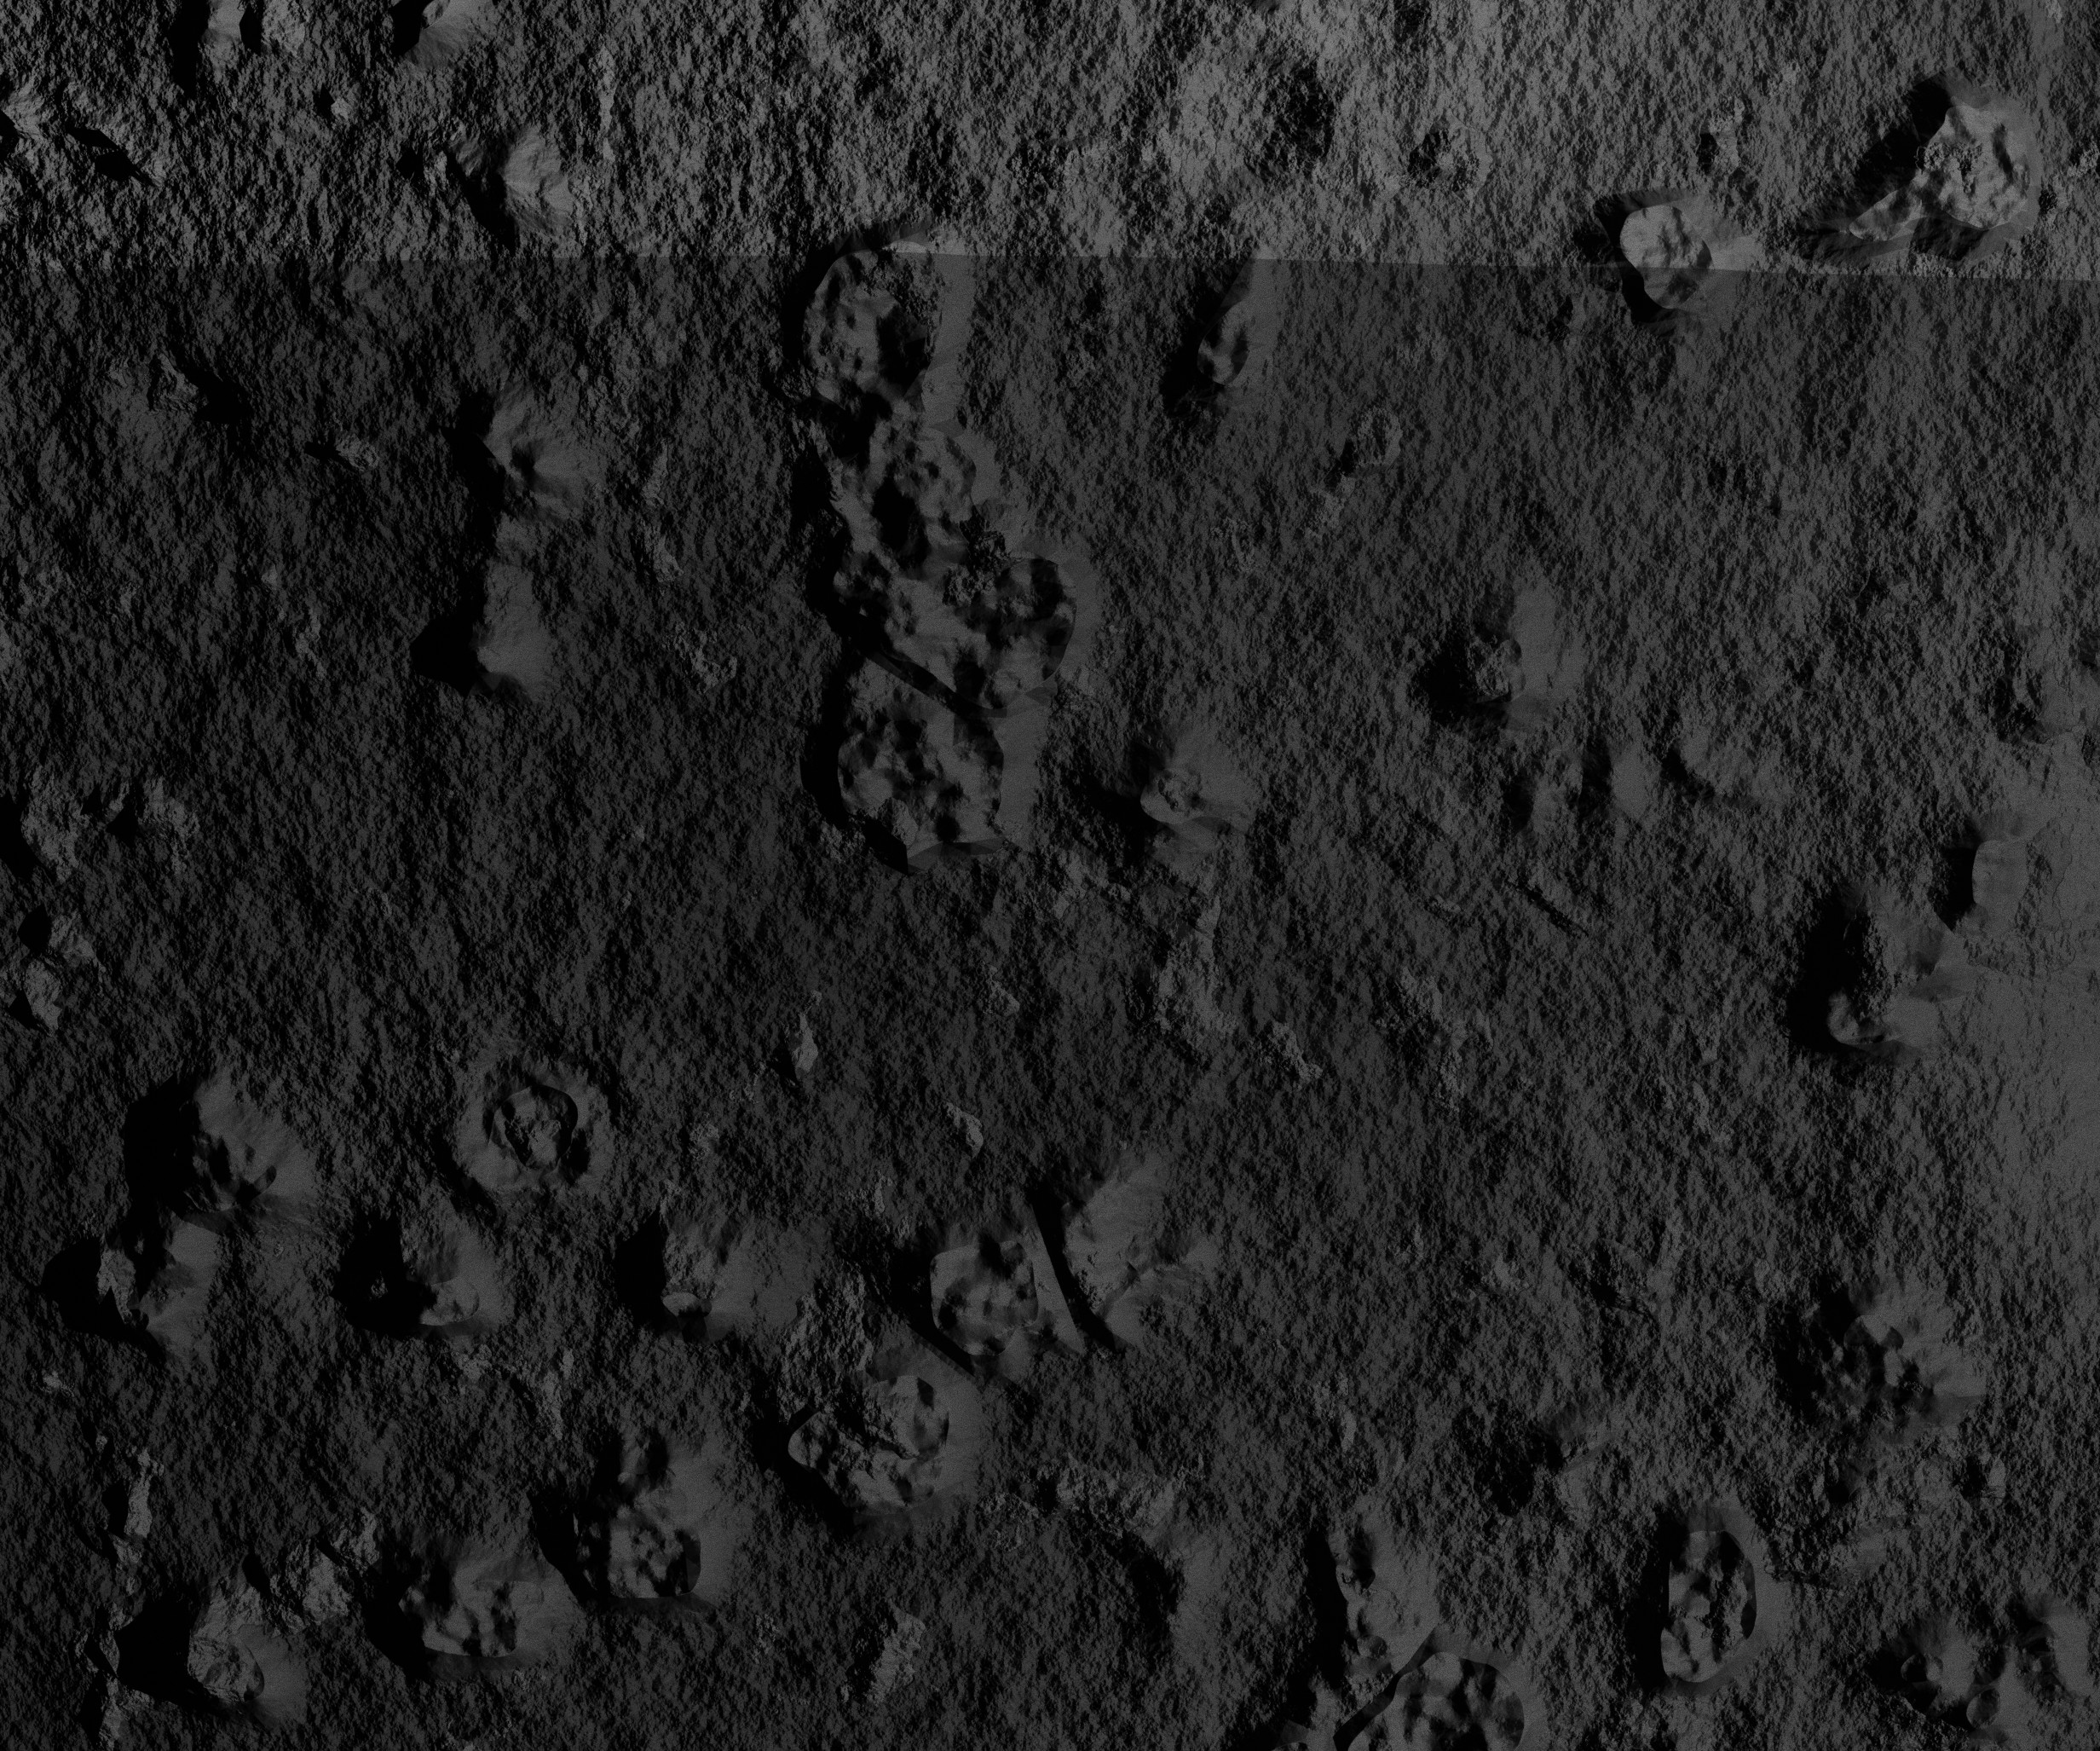
\includegraphics[width=\textwidth]{doc/thesis/0_figures/rendering_artefacts/50_10_SssbOnly_2017-08-15T115845-190000.jpg}
        \caption{}
        \label{fig:render_artefacts_50}
    \end{subfigure}
    \begin{subfigure}[b]{0.32\textwidth}
        \centering
        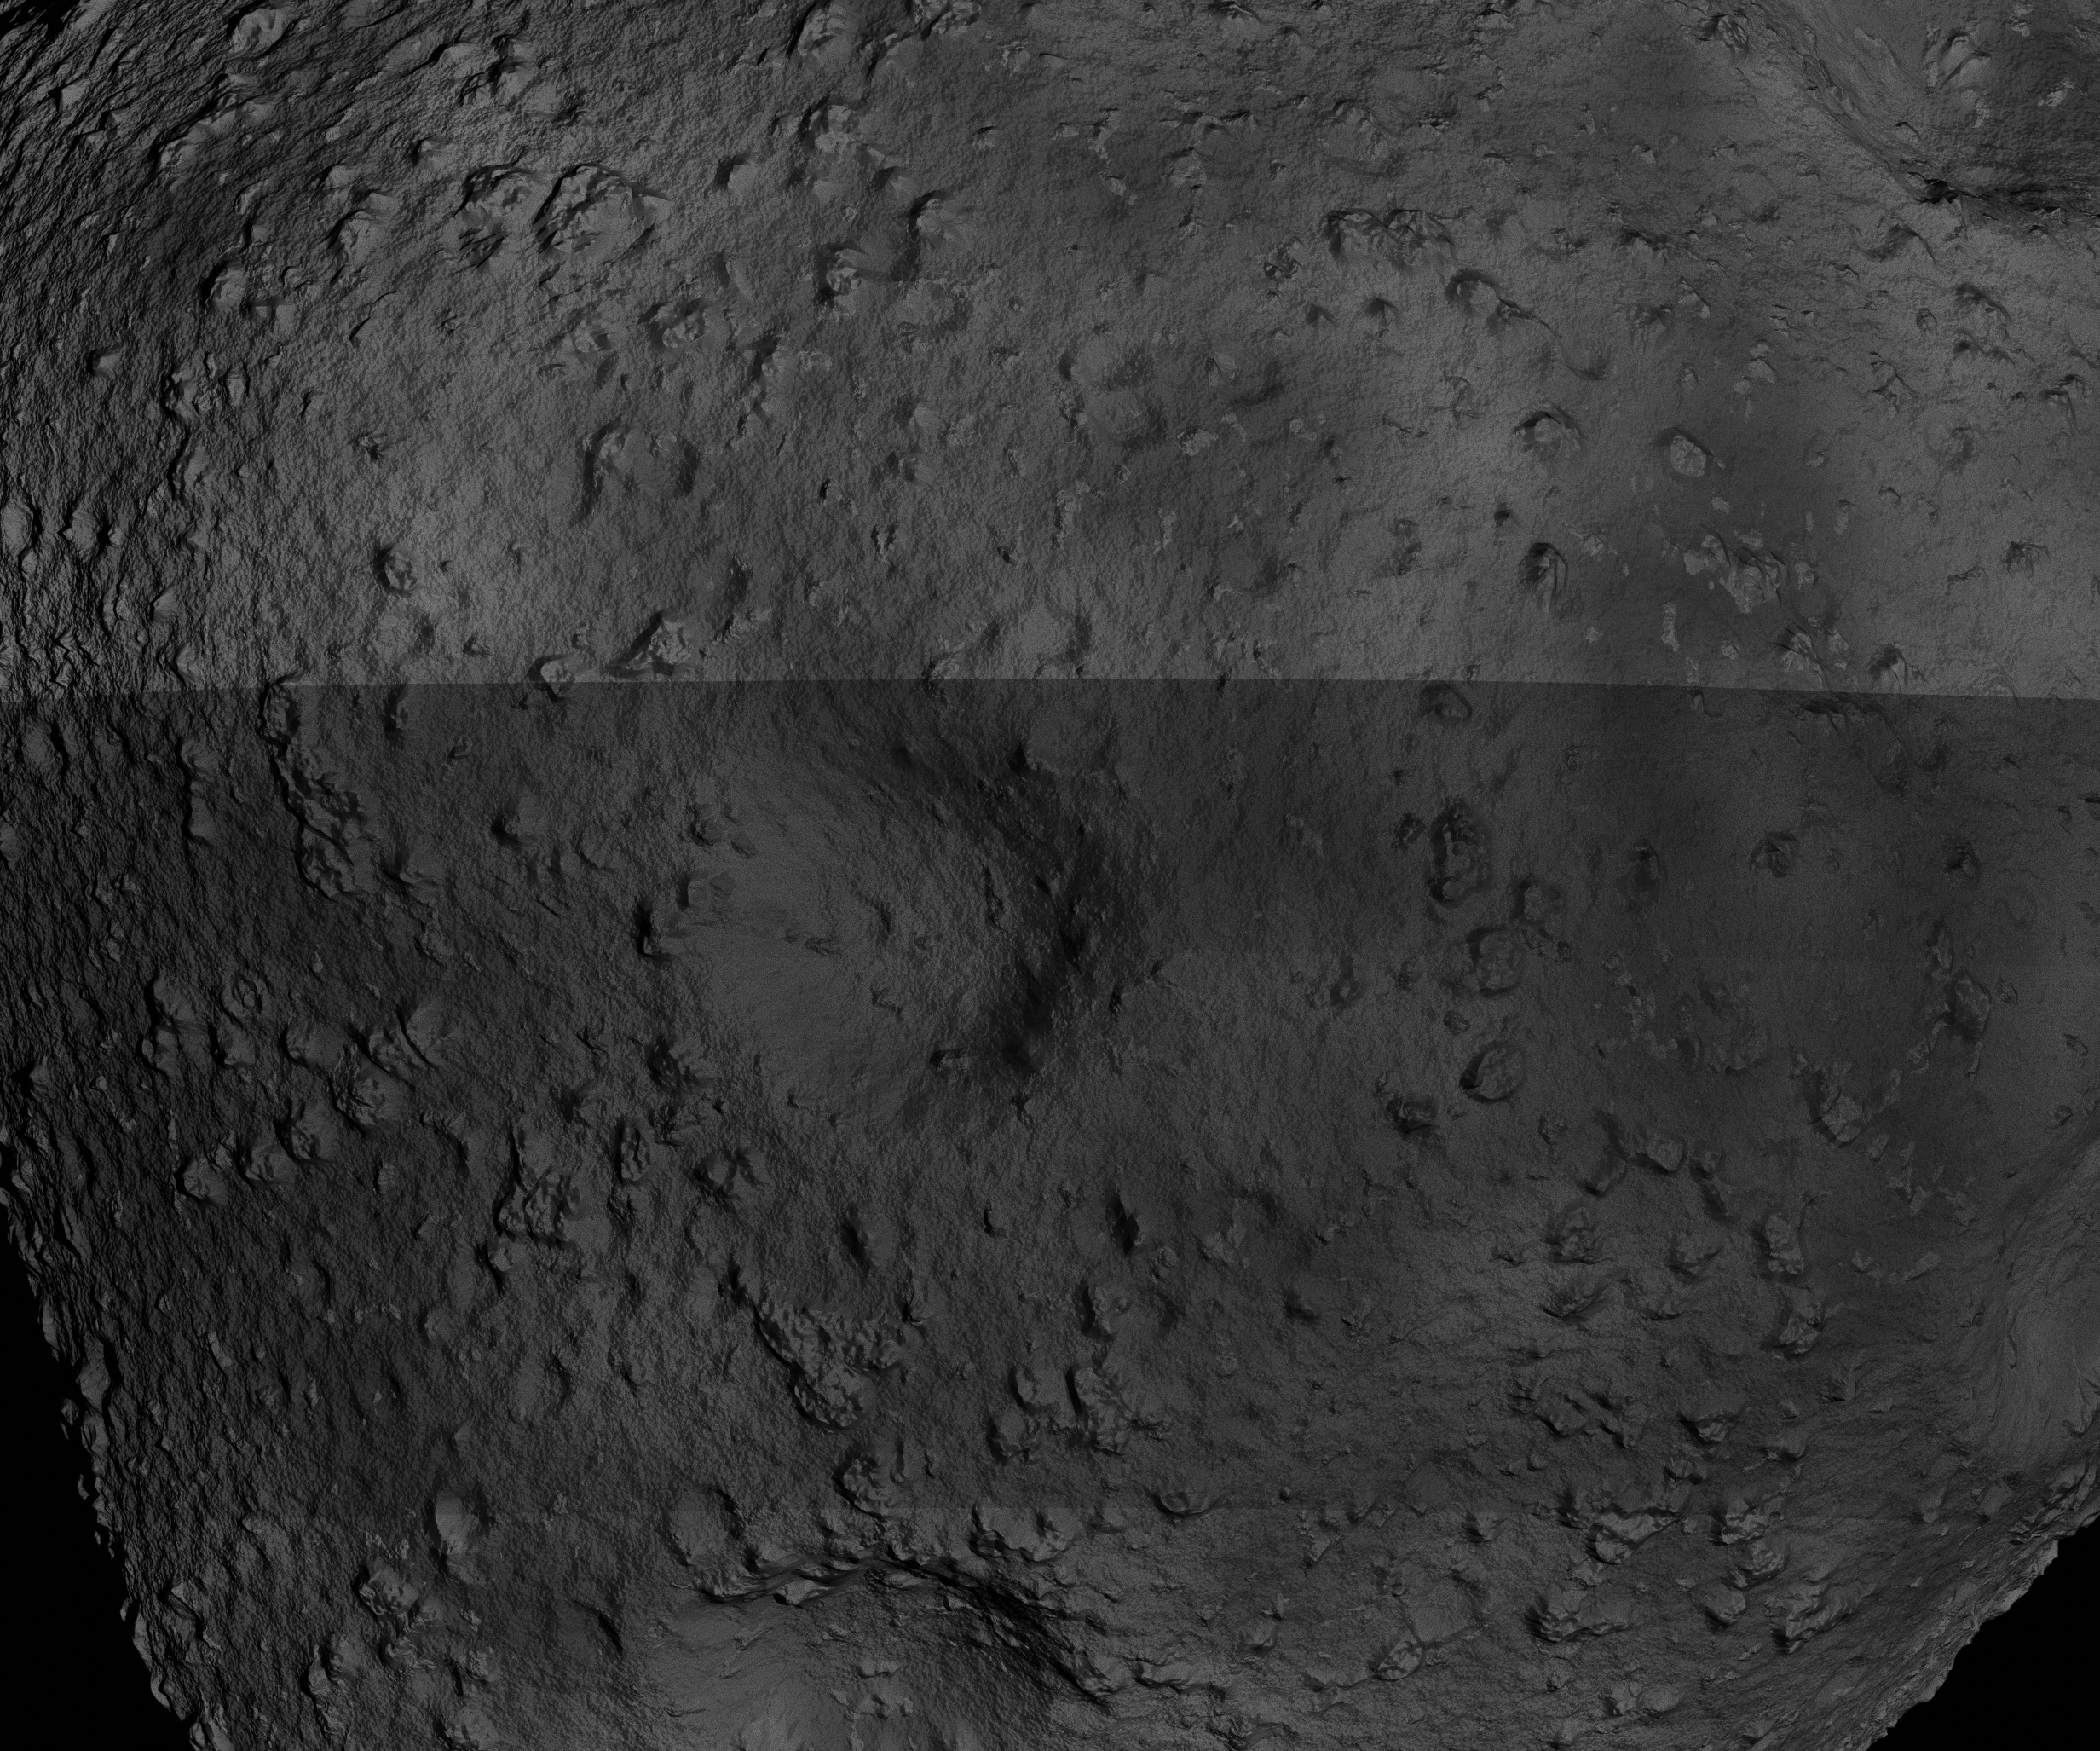
\includegraphics[width=\textwidth]{doc/thesis/0_figures/rendering_artefacts/200_10_SssbOnly_2017-08-15T115845-190000.jpg}
        \caption{}
        \label{fig:render_artefacts_200}
    \end{subfigure}
    \begin{subfigure}[b]{0.32\textwidth}
        \centering
        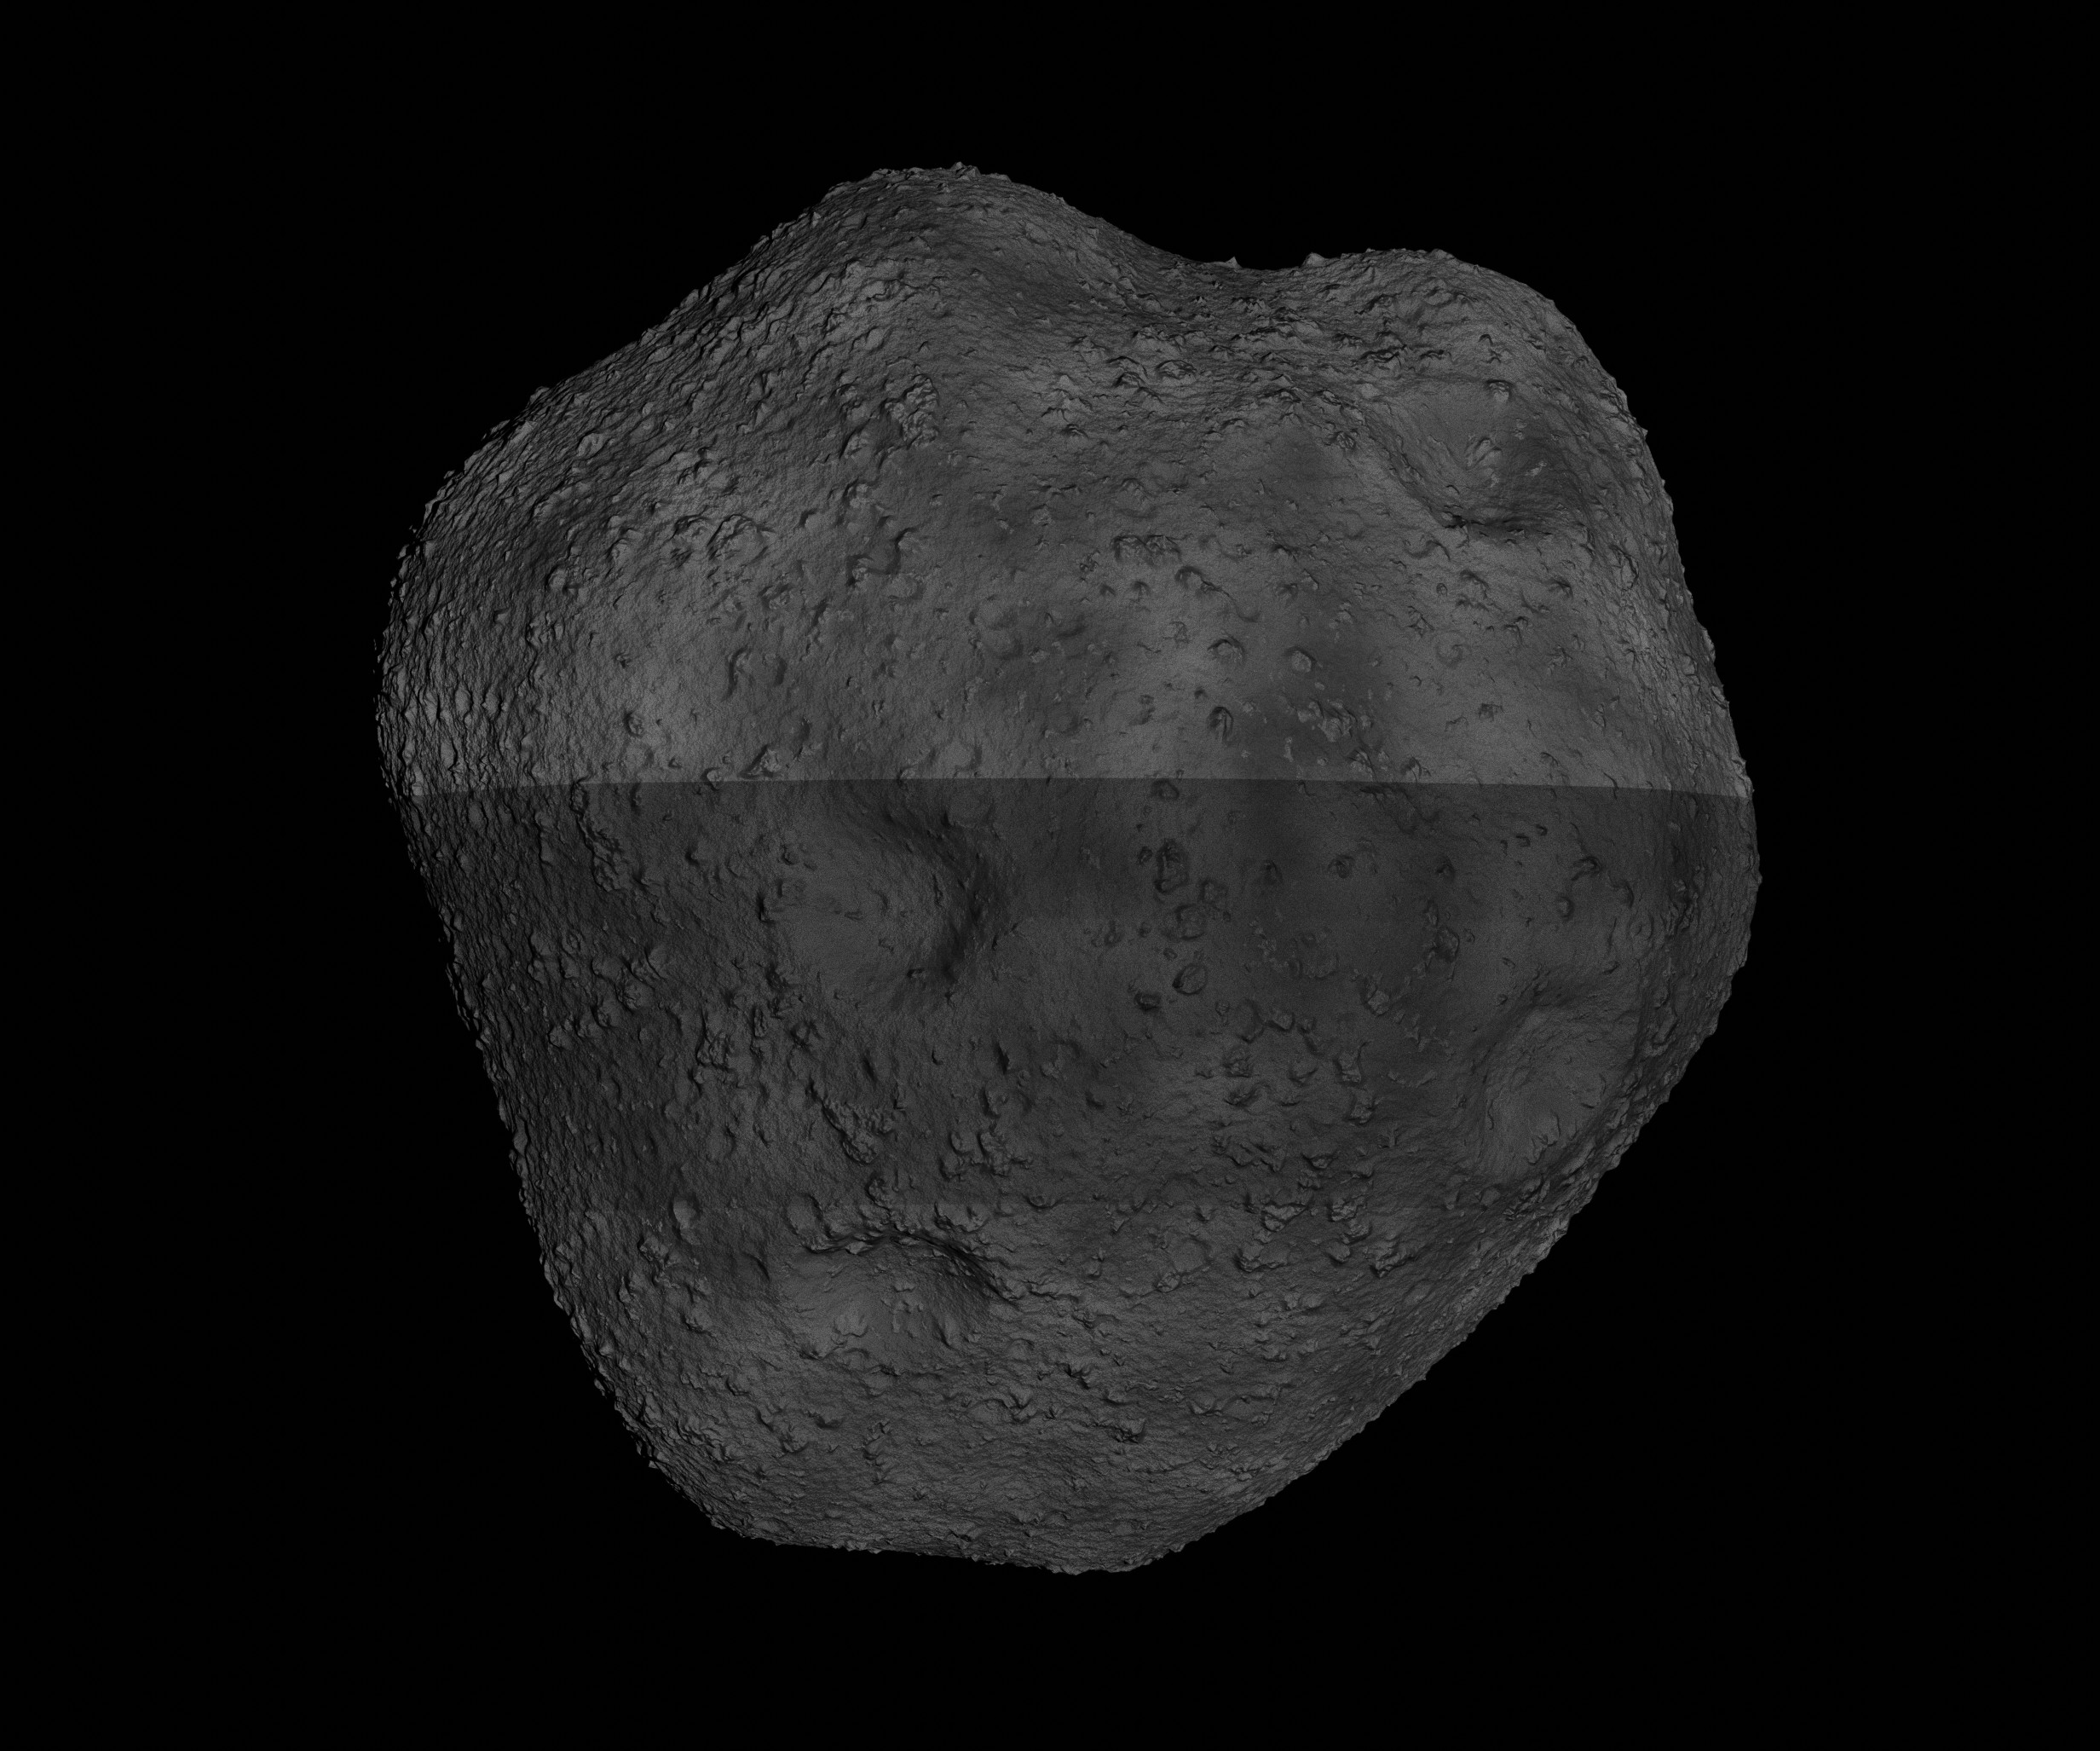
\includegraphics[width=\textwidth]{doc/thesis/0_figures/rendering_artefacts/400_10_SssbOnly_2017-08-15T115845-190000.jpg}
        \caption{}
        \label{fig:render_artefacts_400}
    \end{subfigure}
    \caption{Surface of a \SI{10}{\kilo\meter} \gls{sssb} for varying fly-by distances. Rendering artefacts, the stripes, are visible in all images. (a)~Fly-by distance \SI{50}{\kilo\meter}. (b)~Fly-by distance \SI{200}{\kilo\meter}. (c)~Fly-by distance \SI{400}{\kilo\meter}.}
    \label{fig:render_artefacts}
\end{figure}

A second problem occurred in a \SI{50}{\kilo\meter} fly-by simulation with a \SI{1}{\kilo\meter} \gls{sssb}. A single image was found to be darker than any other image in the data set. Figure~\ref{fig:render_dark} shows three consecutive images. The middle image is overall darker except for a small patch of white pixels. Three pixels are much brighter than any other pixel in the image. The bright pixels are called fireflies~\cite{Valenza2015BlenderCookbook}. Figure~\ref{fig:render_dark} contains composed images for better visibility of the artefact. The fireflies are not introduced by the composition process since they exist in the raw rendered image. No second image with the same issue was found in any other data set thus the problem was not investigated further.

\begin{figure}[htb]
    \centering
        \begin{subfigure}[b]{0.32\textwidth}
            \centering
            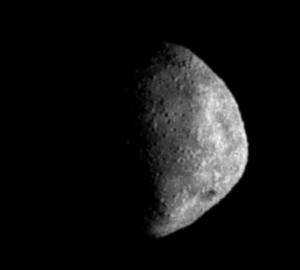
\includegraphics[width=\textwidth]{doc/thesis/0_figures/composition_darkening/50km_Inst_2017-08-15T115816-993000_center.png}
            \label{fig:render_dark_1}
        \end{subfigure}
        \begin{subfigure}[b]{0.32\textwidth}
            \centering
            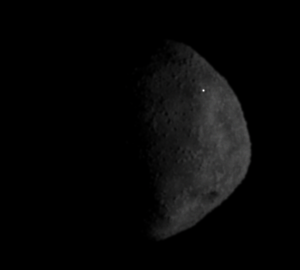
\includegraphics[width=\textwidth]{doc/thesis/0_figures/composition_darkening/Inst_2017-08-15T115818-000000_center.png}
            \label{fig:render_dark_2}
        \end{subfigure}
        \begin{subfigure}[b]{0.32\textwidth}
            \centering
            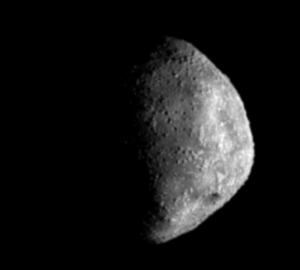
\includegraphics[width=\textwidth]{doc/thesis/0_figures/composition_darkening/Inst_2017-08-15T115819-007000_center.png}
            \label{fig:render_dark_3}
        \end{subfigure}
    \caption{Overall darkened \gls{sssb} image due to three pixels being much brighter. These pixels are referred to as fireflies~\cite{Valenza2015BlenderCookbook}. All three images are composed images for better visibility of the artefact. The images are cropped to display the \gls{sssb} nucleus and artefact better.}
    \label{fig:render_dark}
\end{figure}

\clearpage

\subsection{Compression} \label{sec:results_comp}
The \gls{sispo} software package was used to study the effects of compression in different scenarios. The scenarios are presented in Table~\ref{tab:sim_params}. Two compression algorithms were used to study compression effects. The \gls{png} format was used because of its wide support among different software packages and \gls{jp2} is used as an improved version over commonly used \gls{jpeg}. The \gls{png} and \gls{jp2} formats were selected as general examples to characterise compression effects on reconstruction. Neither \gls{png} nor \gls{jp2} are intended to represent image processing on-board a spacecraft. Scenarios with varying \gls{sssb} nucleus sizes and fly-by distance were simulated. 

The comparison of the different compression algorithms is based on several parameters. The used parameters are the size of the compressed image series, the number of points in the dense reconstructed point cloud, the number of vertices and the number of faces of the refined reconstructed model. These outputs relate to the level of detail of the rendered images since \gls{sfm} algorithms rely on surface details for reconstruction.

\Gls{jp2} quality levels presented in the results are the quality levels as defined in the \gls{jp2} implementation used by OpenCV, i.e. ranging from 0 to 1000.

\subsubsection{Image Quality Comparison} \label{sec:img_quali_comp}
A specific image was selected to compare image quality after different levels of compression. Since reconstruction is mostly influenced by features, a scene with a distance of \SI{50}{\kilo\meter} to the a \SI{1}{\kilo\meter} nucleus was selected for comparison. Overall images contain the entire \gls{sssb} in the \gls{fov}. Close-up images show the area highlighted by the red frame in Figure~\ref{fig:img_quality_frame}. Overall images show compression effects on an entire scene while close-up images reveal compression effects on surface details. Difference images and histograms are used to investigate compression effects in more detail. 

Difference images are created by converting the \gls{rgb} images to greyscale and calculating the L2-norm after subtracting each pixel from the respective pixel value of the \gls{png} greyscale image. The result is a greyscale difference image showing the L2-norm differences. The zero values in histograms were removed to only show alterations by compression. Therefore, total number of altered pixels and the percentage relative to the original image are presented in the histogram.

\begin{figure}[htb]
    \centering
    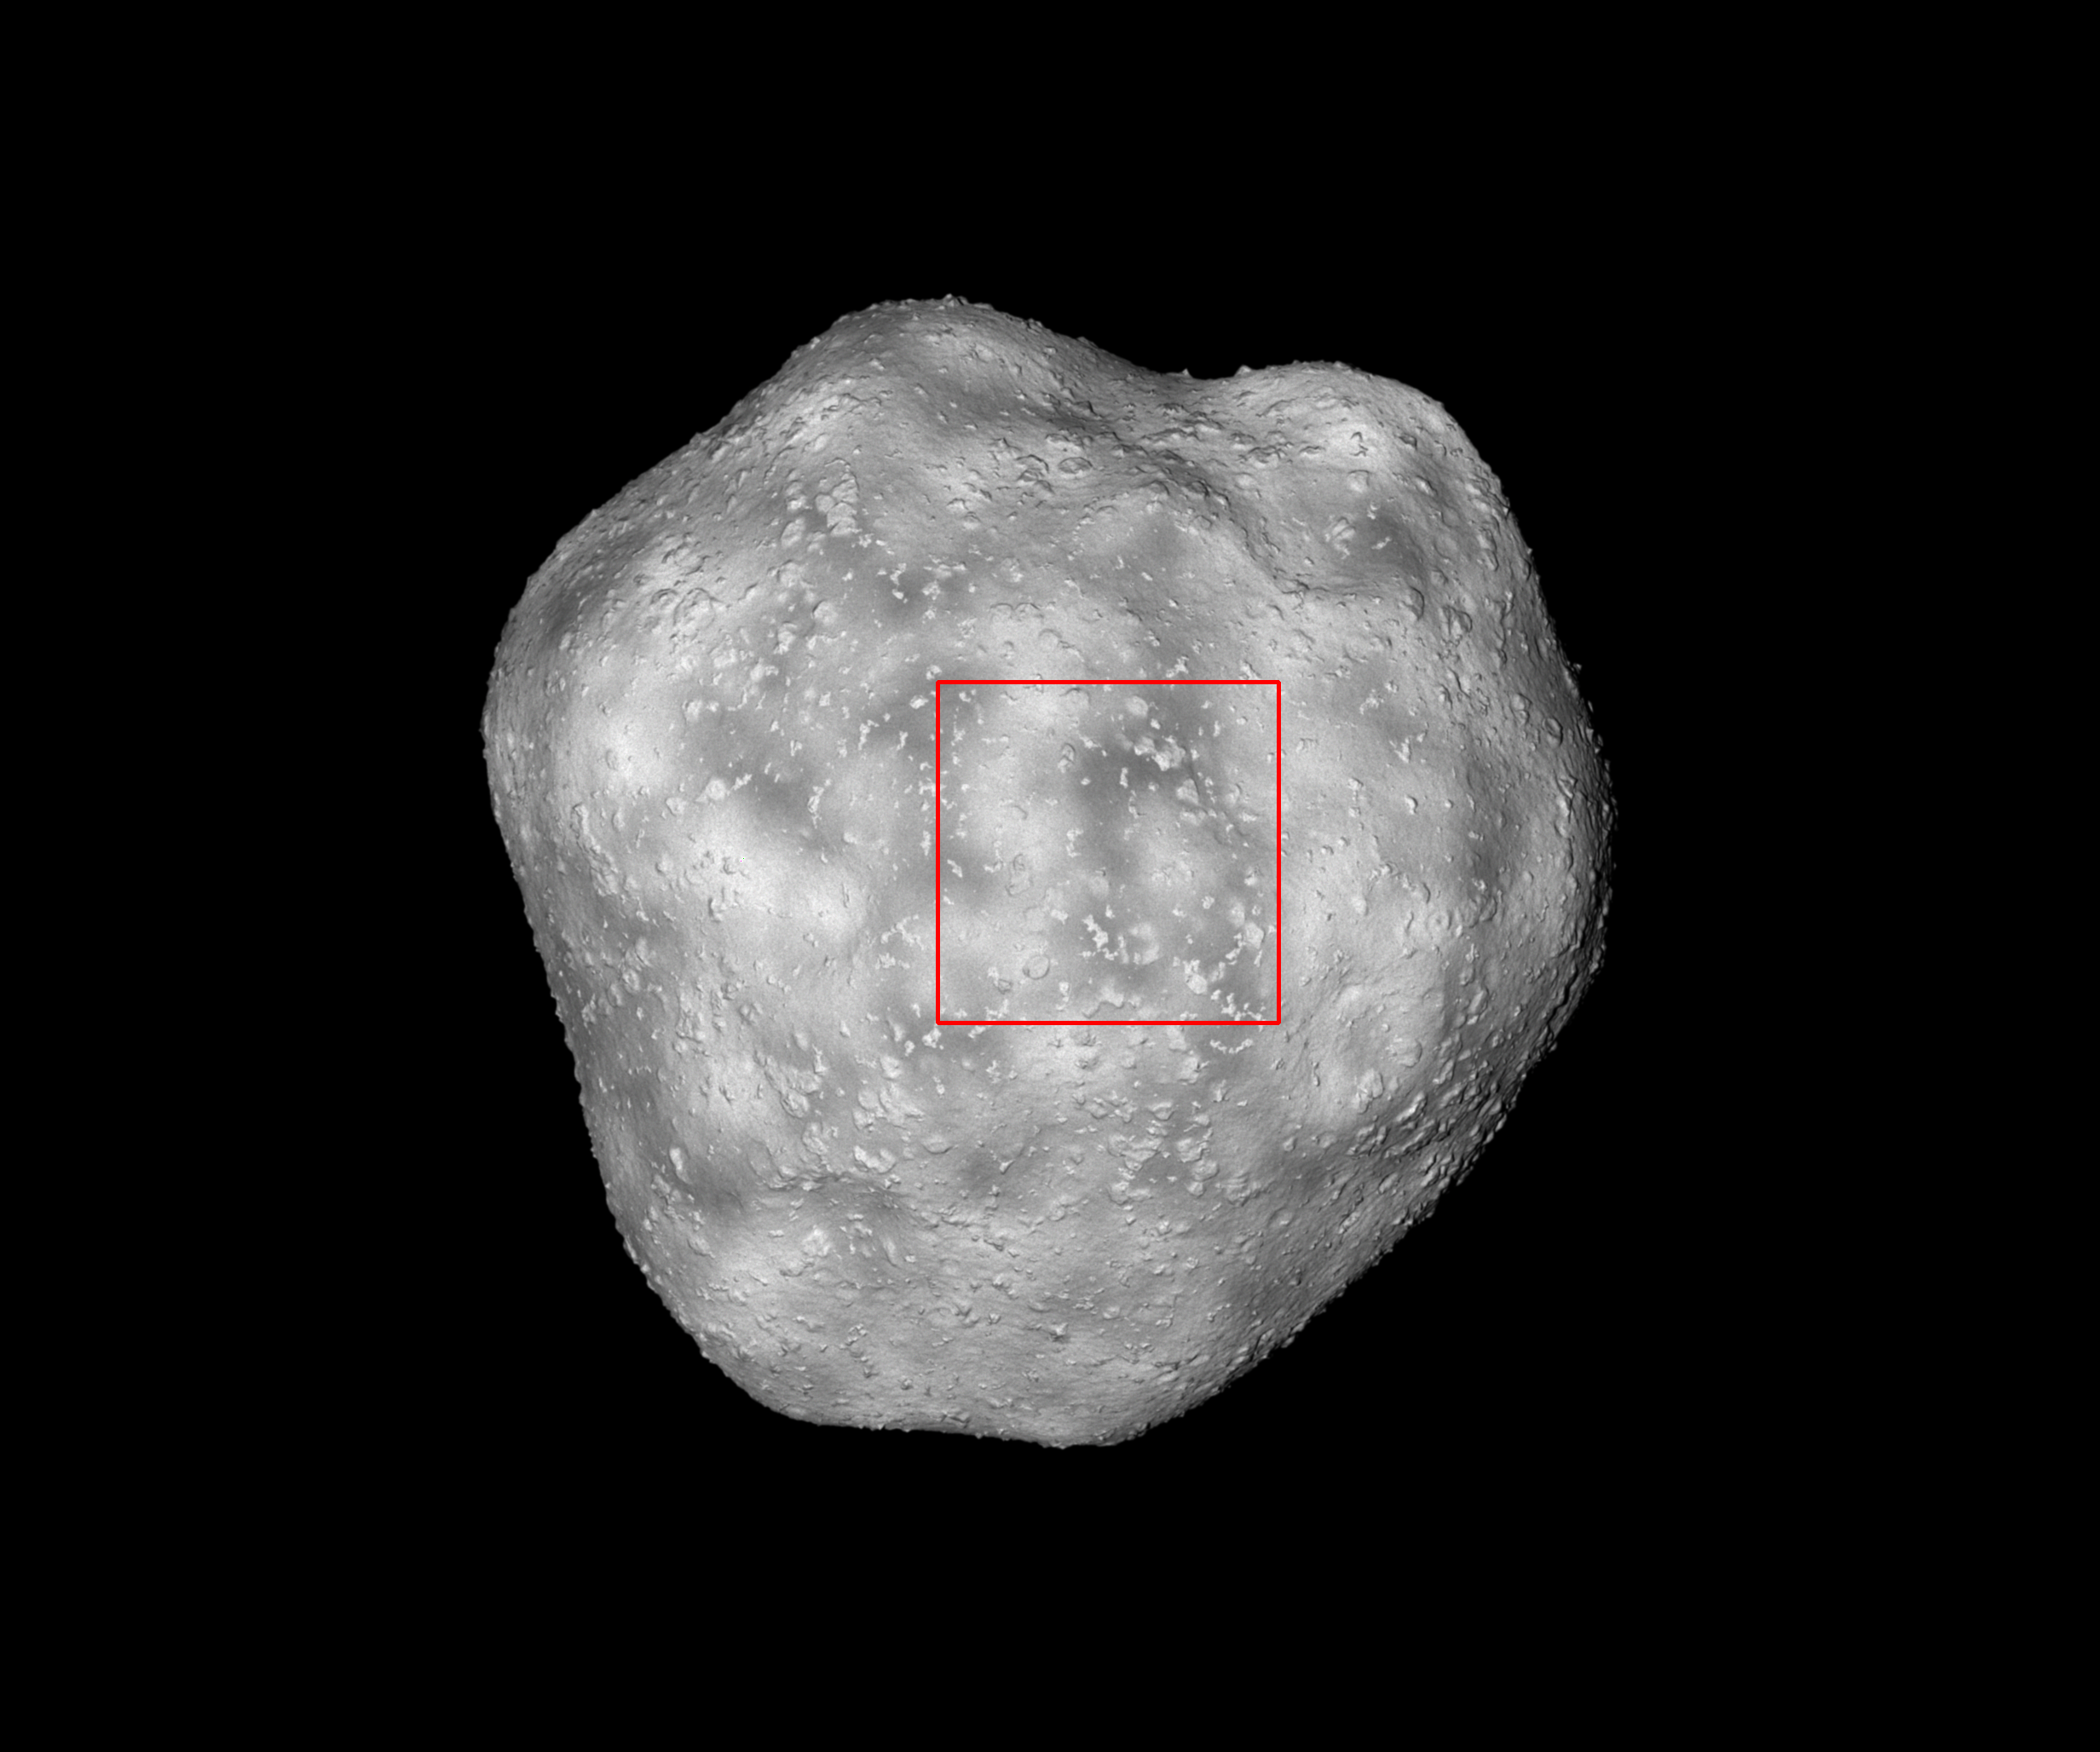
\includegraphics[width=.7\textwidth]{doc/thesis/0_figures/compare_quality/set1/jp2_1000_frame}
    \caption{Scene used for quality comparison. The area highlighted in red is studied up closer. The specific area was selected since it includes a wide range of colours and various sized surface features.}
    \label{fig:img_quality_frame}
\end{figure}

Figures~\ref{fig:img_quality_comp_jp2_1} to \ref{fig:img_quality_comp_jp2_1000} show the compressed overall image, difference histograms and the difference images after compression with \gls{jp2} with quality levels \SI{1}{}, \SI{5}{}, \SI{10}{}, \SI{100}{} and \SI{1000}{}. Quality level \SI{5}{} is used since most changes due to compression occur at low quality levels.

\begin{figure}[htb]
    \centering
    \begin{subfigure}[b]{0.48\textwidth}
        \centering
        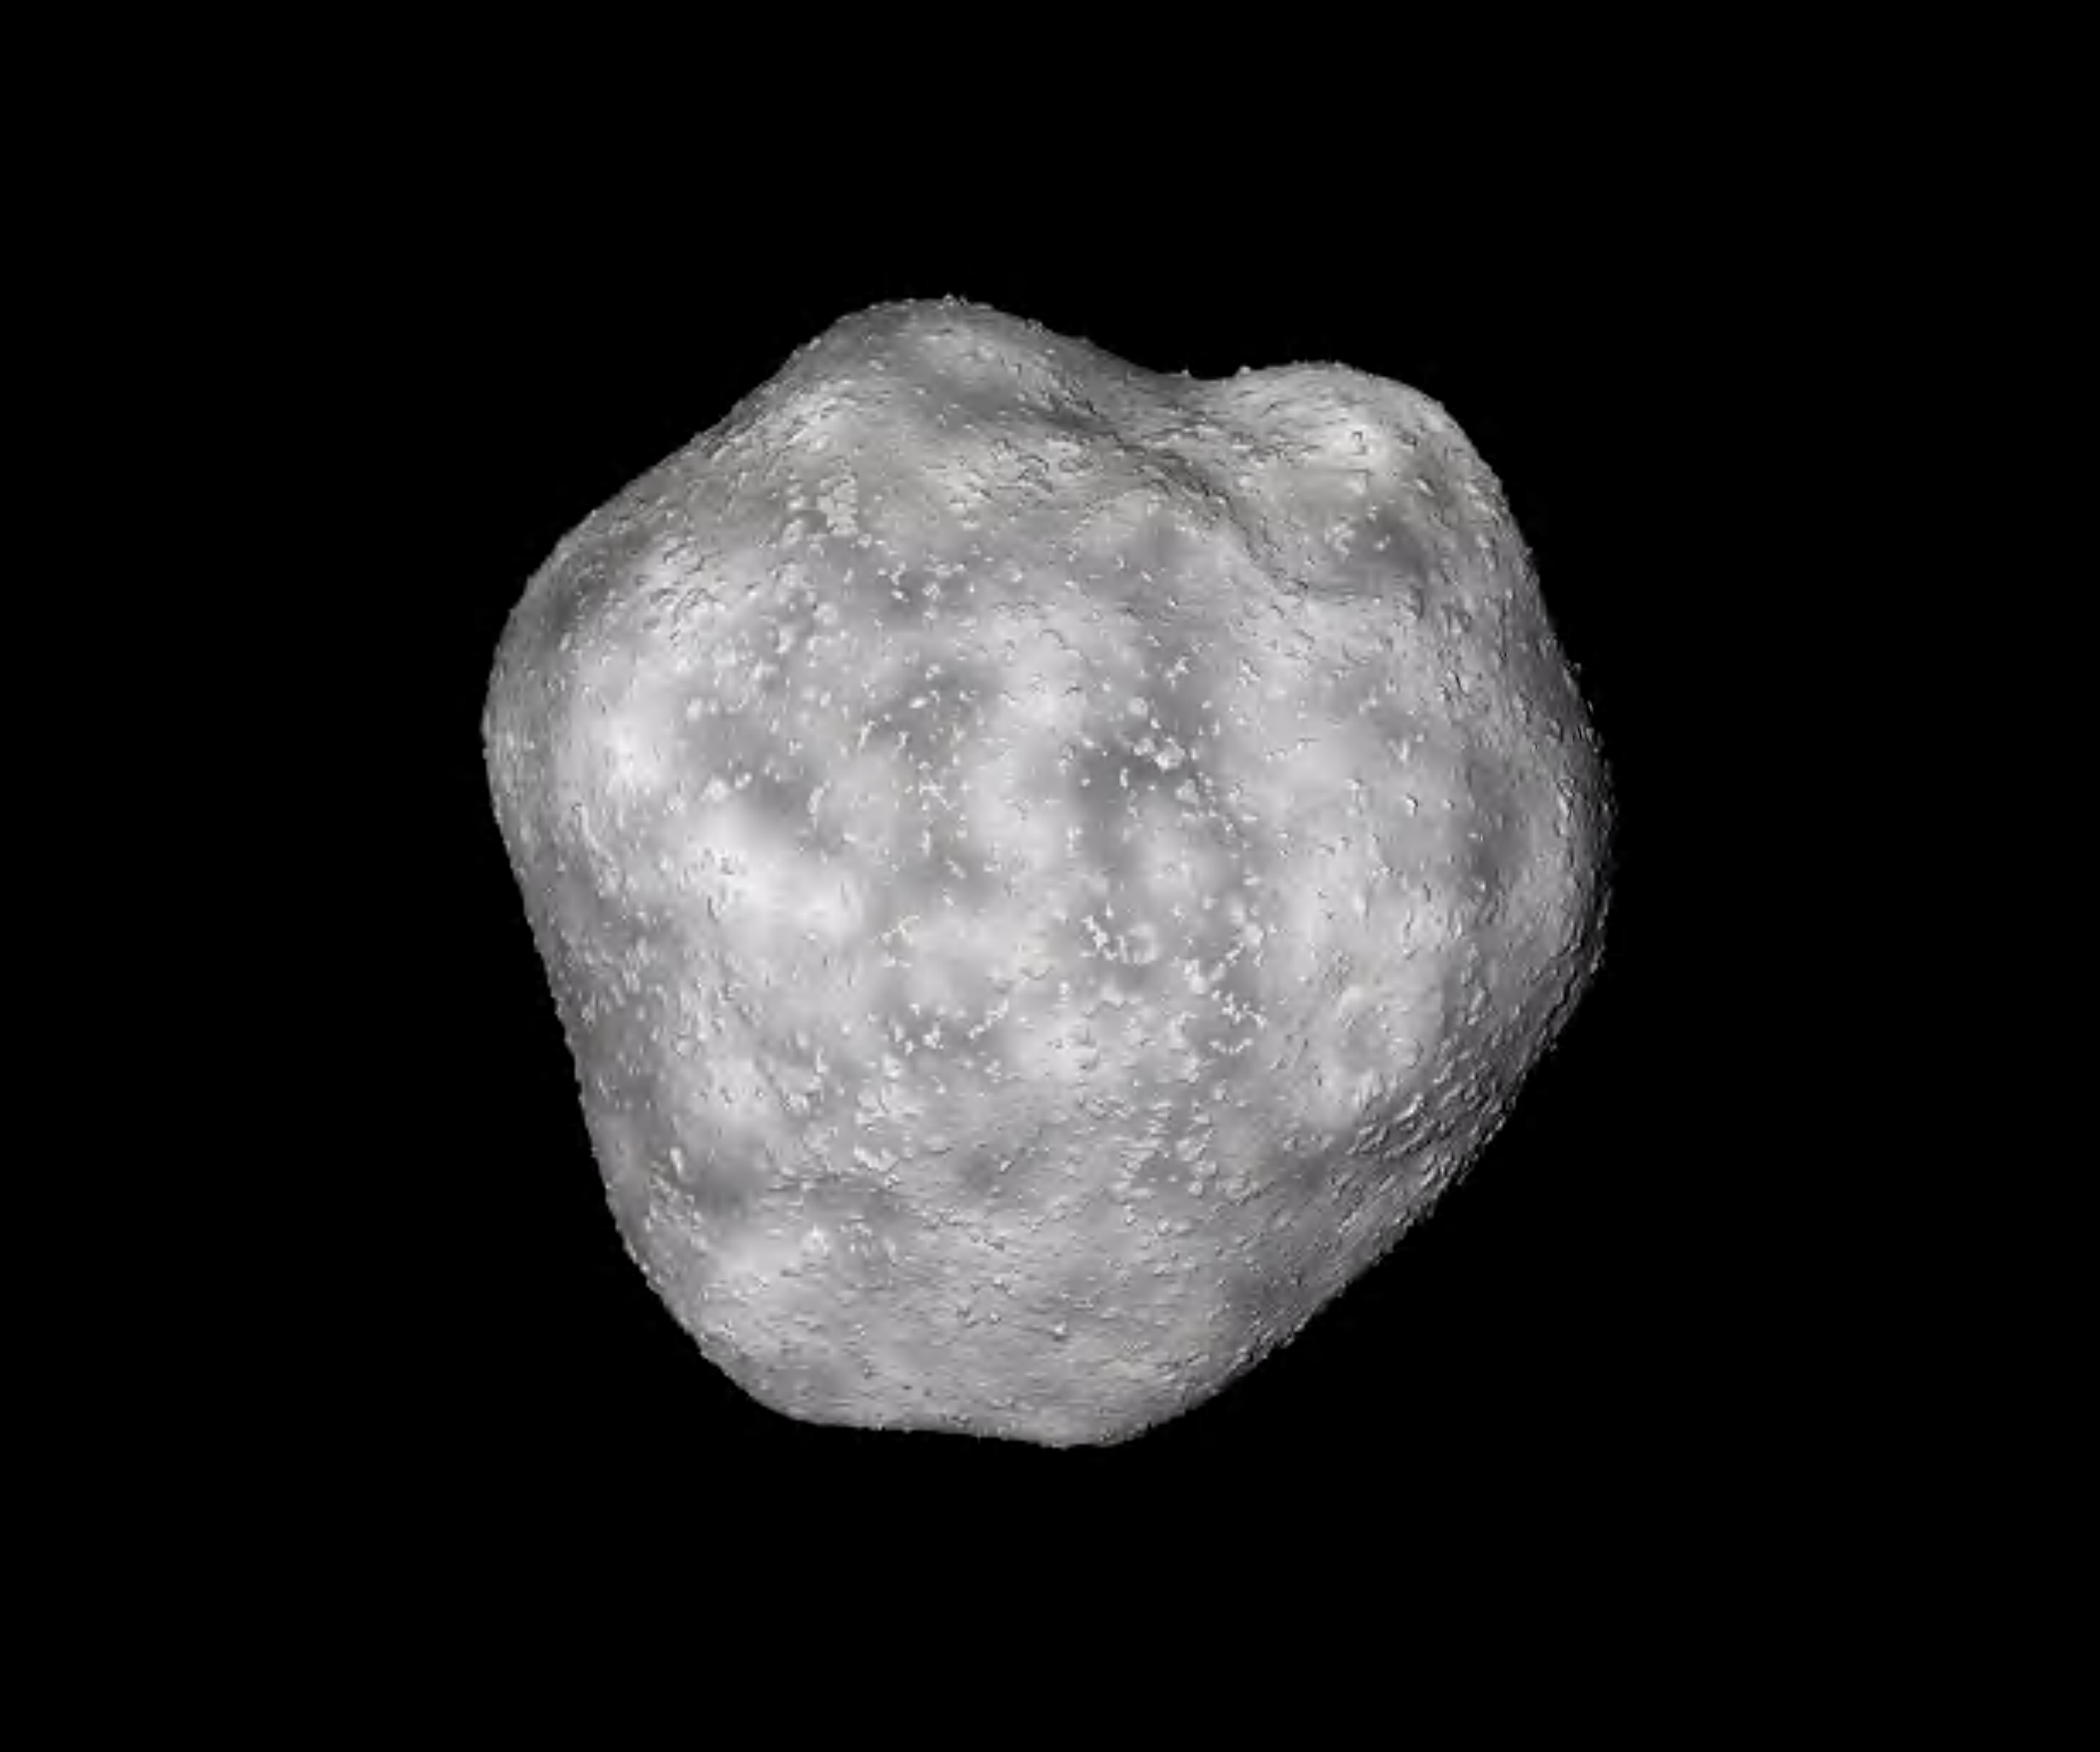
\includegraphics[width=\textwidth]{doc/thesis/0_figures/compare_quality/set1/jp2_1}
        \caption{}
        \label{fig:img_quality_comp_jp2_1_orig}
    \end{subfigure}
    \begin{subfigure}[b]{0.48\textwidth}
        \centering
        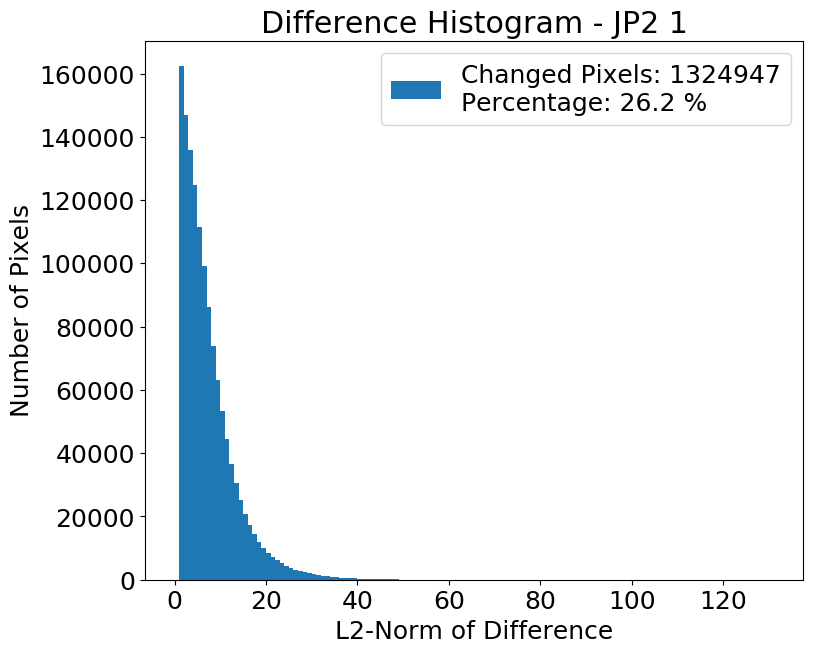
\includegraphics[width=\textwidth]{doc/thesis/0_figures/compare_quality/set1/jp2_1_diff_histogram}
        \caption{}
        \label{fig:img_quality_comp_jp2_1_histo}
    \end{subfigure}
    \\
    \begin{subfigure}[b]{0.48\textwidth}
        \centering
        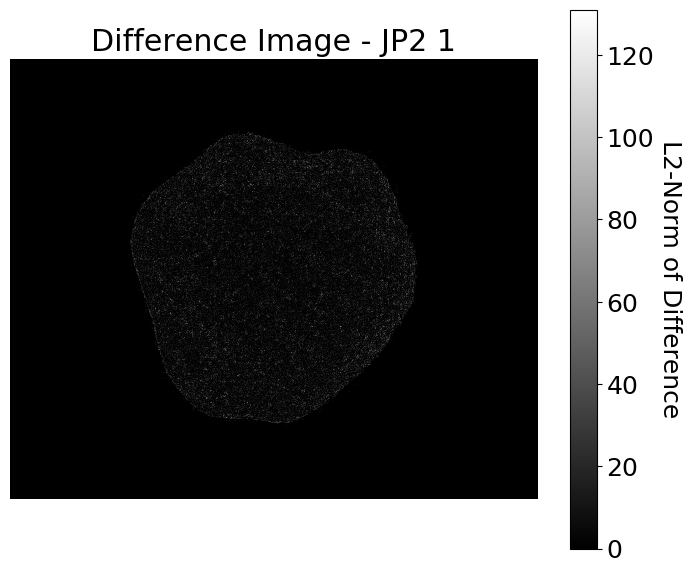
\includegraphics[width=\textwidth]{doc/thesis/0_figures/compare_quality/set1/jp2_1_diff_heatmap}
        \caption{}
        \label{fig:img_quality_comp_jp2_1_diff}
    \end{subfigure}
    \begin{subfigure}[b]{0.48\textwidth}
        \centering
        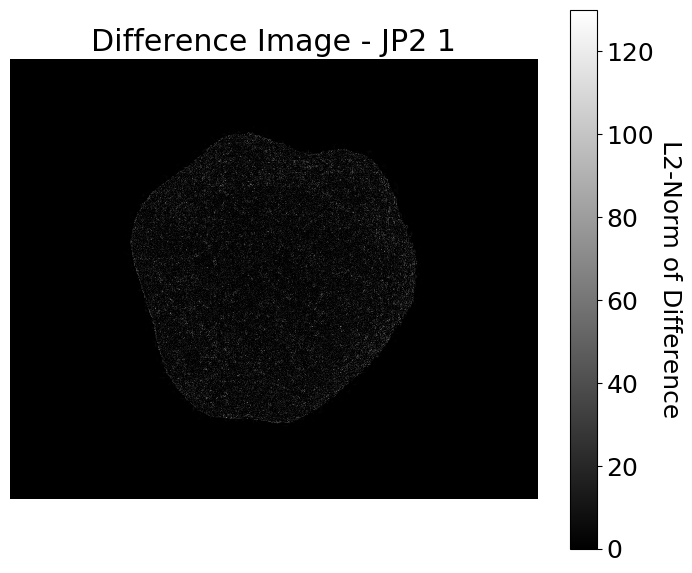
\includegraphics[width=\textwidth]{doc/thesis/0_figures/compare_quality/set1/jp2_1_diff_heatmap_rel}
        \caption{}
        \label{fig:img_quality_comp_jp2_1_diff_rel}
    \end{subfigure}
    \caption{Overall rendered image after compression with \gls{jp2} quality level 1. The L2-norm is applied to the difference between the greyscale images of the lossless and respective lossy image. (a)~Image after lossy compression. (b)~Histogram of L2-norms of differences. (c)~L2-norm difference image with a colour scale from $0$ to $131$ for comparison between various compression levels. (d)~L2-norm difference image with a colour scale from $0$ to the maximum L2-norm value for better visibility of compression effects.}
    \label{fig:img_quality_comp_jp2_1}
\end{figure}


\begin{figure}[htb]
    \centering
    \begin{subfigure}[b]{0.48\textwidth}
        \centering
        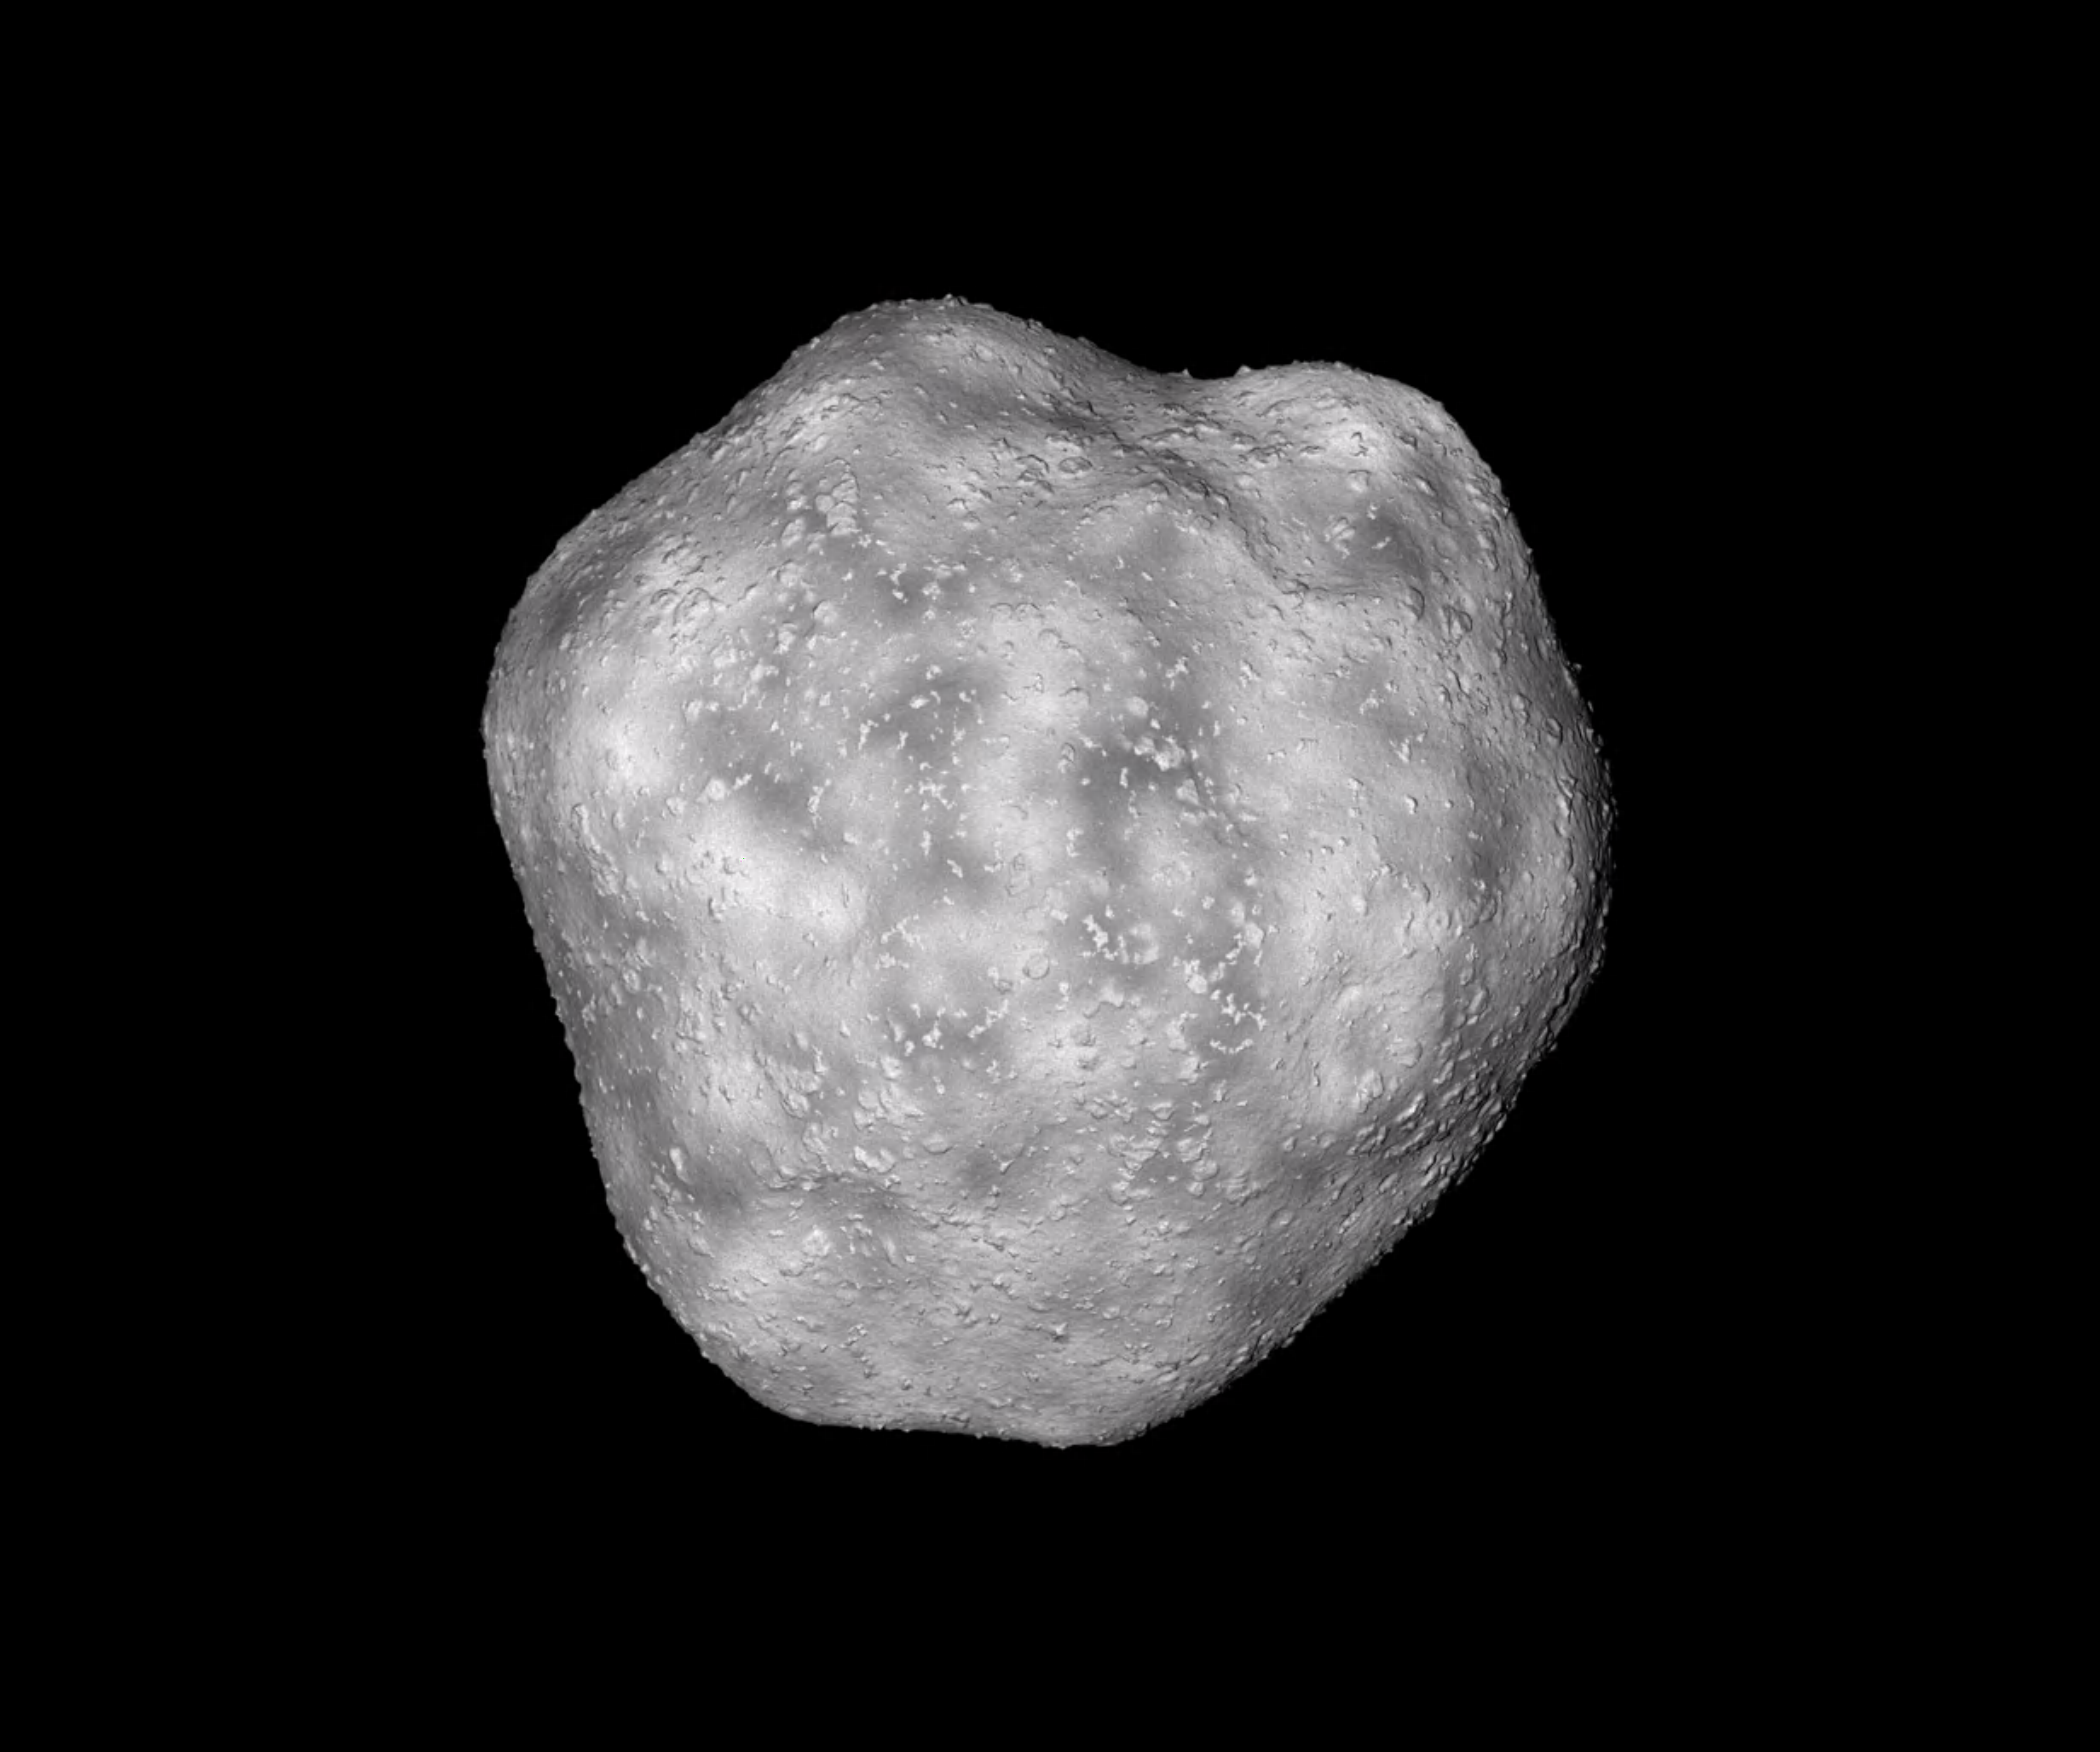
\includegraphics[width=\textwidth]{doc/thesis/0_figures/compare_quality/set1/jp2_5}
        \caption{}
        \label{fig:img_quality_comp_jp2_5_orig}
    \end{subfigure}
    \begin{subfigure}[b]{0.48\textwidth}
        \centering
        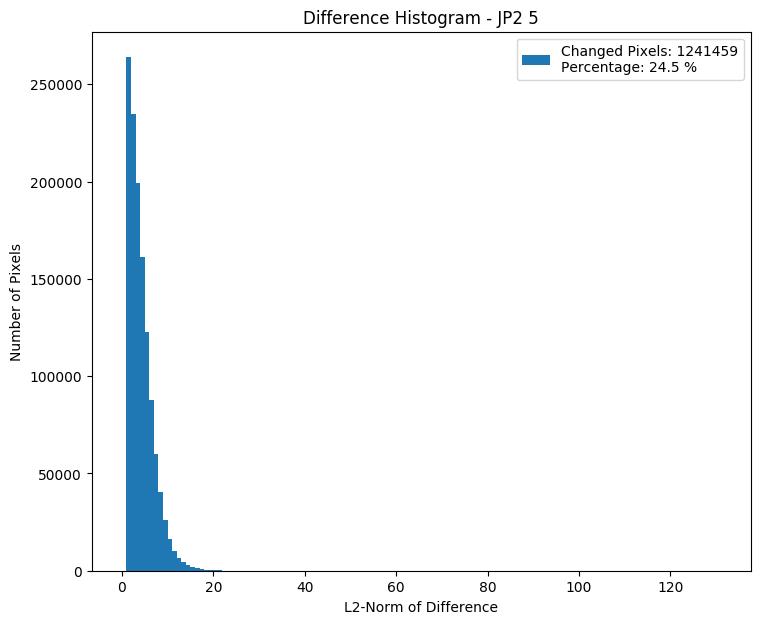
\includegraphics[width=\textwidth]{doc/thesis/0_figures/compare_quality/set1/jp2_5_diff_histogram}
        \caption{}
        \label{fig:img_quality_comp_jp2_5_histo}
    \end{subfigure}
    \\
    \begin{subfigure}[b]{0.48\textwidth}
        \centering
        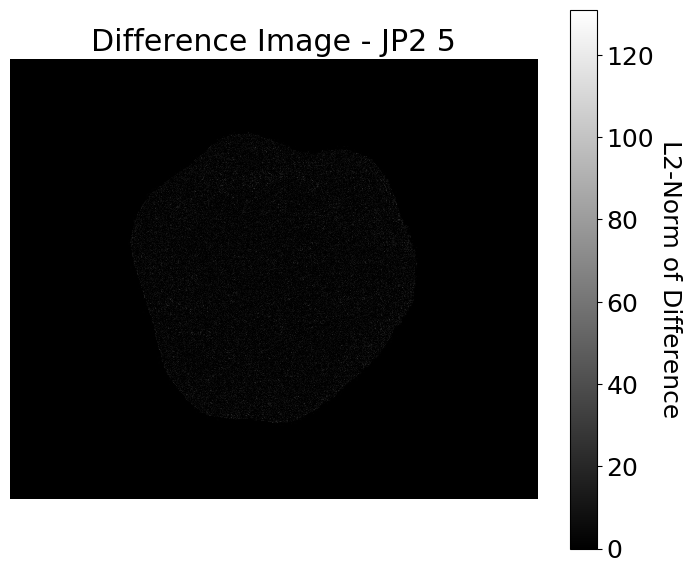
\includegraphics[width=\textwidth]{doc/thesis/0_figures/compare_quality/set1/jp2_5_diff_heatmap}
        \caption{}
        \label{fig:img_quality_comp_jp2_5_diff}
    \end{subfigure}
    \begin{subfigure}[b]{0.48\textwidth}
        \centering
        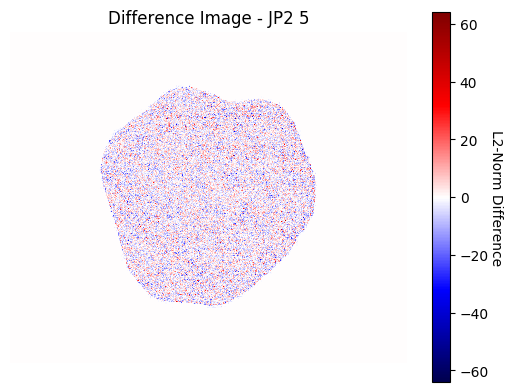
\includegraphics[width=\textwidth]{doc/thesis/0_figures/compare_quality/set1/jp2_5_diff_heatmap_rel}
        \caption{}
        \label{fig:img_quality_comp_jp2_5_diff_rel}
    \end{subfigure}
    \caption{Overall rendered image after compression with \gls{jp2} quality level 5. The L2-norm is applied to the difference between the greyscale images of the lossless and respective lossy image. (a) Image after lossy compression. (b) Histogram of L2-norms of differences. (c) L2-norm difference image with a colour scale from $0$ to $131$ for comparison between various compression levels. (d) L2-norm difference image with a colour scale from $0$ to the maximum L2-norm value for better visibility of compression effects.}
    \label{fig:img_quality_comp_jp2_5}
\end{figure}


\begin{figure}[htb]
    \centering
    \begin{subfigure}[b]{0.48\textwidth}
        \centering
        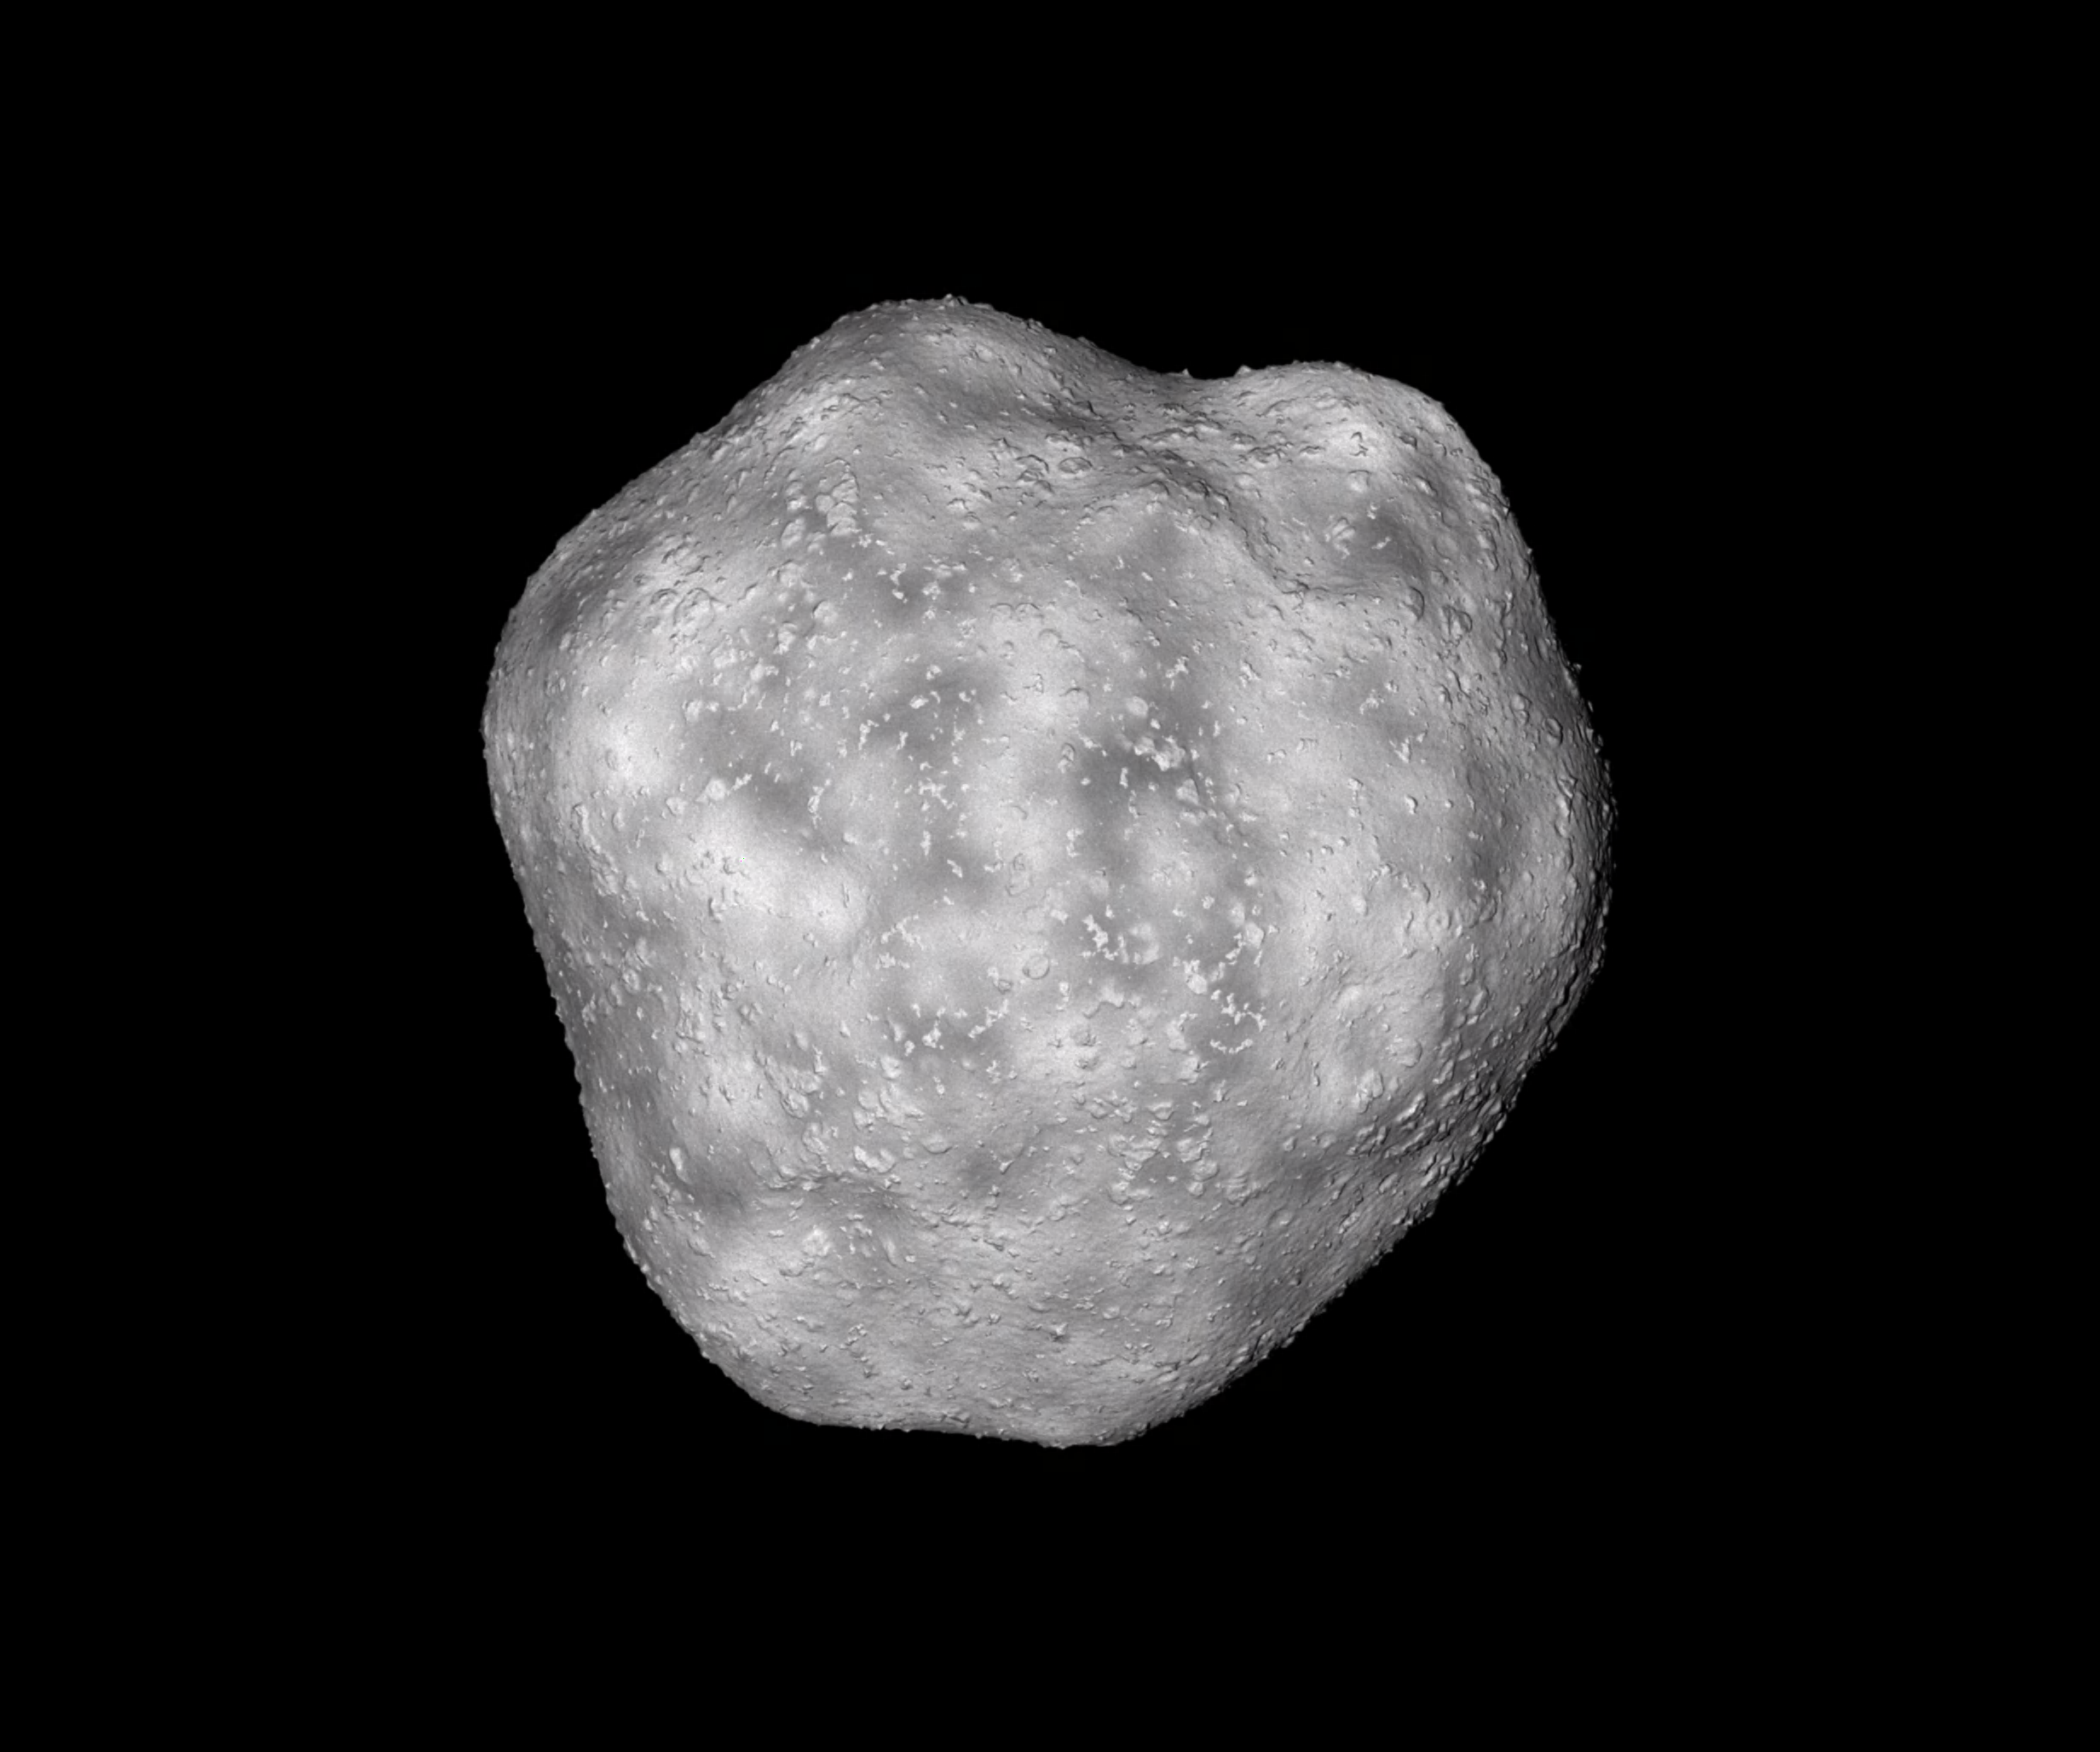
\includegraphics[width=\textwidth]{doc/thesis/0_figures/compare_quality/set1/jp2_10}
        \caption{}
        \label{fig:img_quality_comp_jp2_10_orig}
    \end{subfigure}
    \begin{subfigure}[b]{0.48\textwidth}
        \centering
        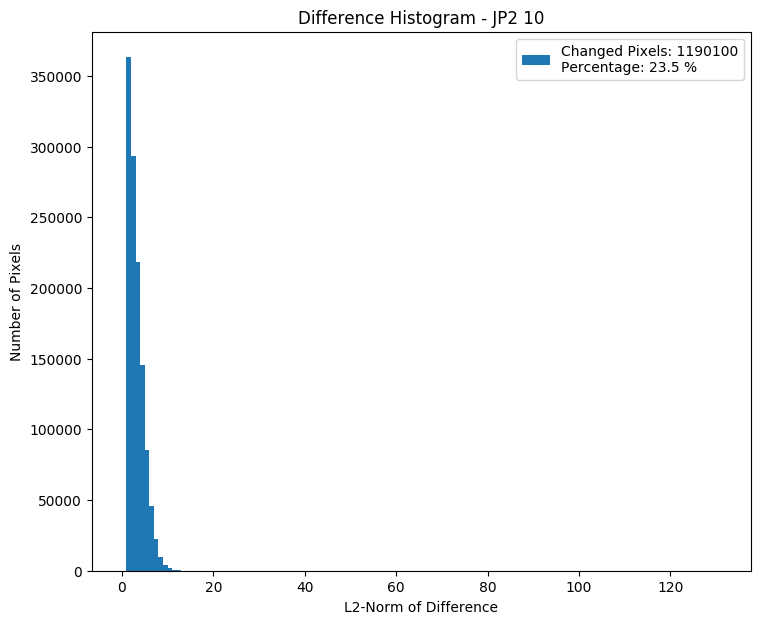
\includegraphics[width=\textwidth]{doc/thesis/0_figures/compare_quality/set1/jp2_10_diff_histogram}
        \caption{}
        \label{fig:img_quality_comp_jp2_10_histo}
    \end{subfigure}
    \\
    \begin{subfigure}[b]{0.48\textwidth}
        \centering
        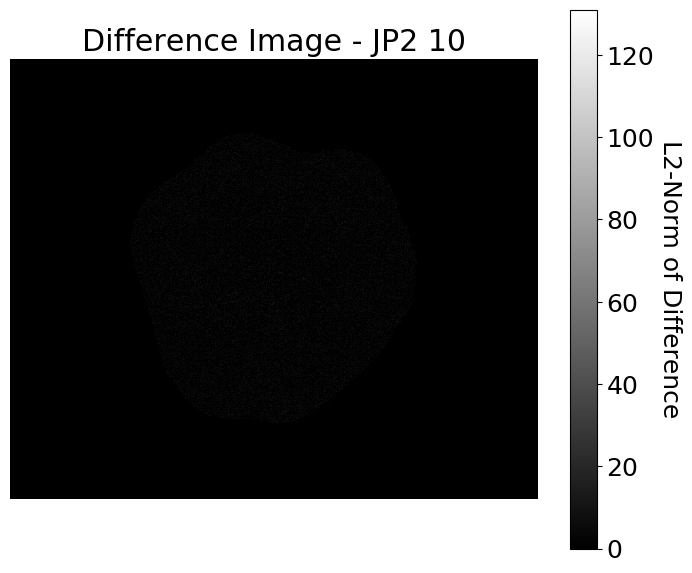
\includegraphics[width=\textwidth]{doc/thesis/0_figures/compare_quality/set1/jp2_10_diff_heatmap}
        \caption{}
        \label{fig:img_quality_comp_jp2_10_diff}
    \end{subfigure}
    \begin{subfigure}[b]{0.48\textwidth}
        \centering
        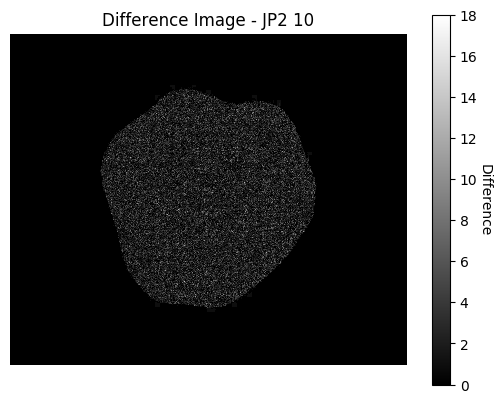
\includegraphics[width=\textwidth]{doc/thesis/0_figures/compare_quality/set1/jp2_10_diff_heatmap_rel}
        \caption{}
        \label{fig:img_quality_comp_jp2_10_diff_rel}
    \end{subfigure}
    \caption{Overall rendered image after compression with \gls{jp2} quality level 10. The L2-norm is applied to the difference between the greyscale images of the lossless and respective lossy image. (a) Image after lossy compression. (b) Histogram of L2-norms of differences. (c) L2-norm difference image with a colour scale from $0$ to $131$ for comparison between various compression levels. (d) L2-norm difference image with a colour scale from $0$ to the maximum L2-norm value for better visibility of compression effects.}
    \label{fig:img_quality_comp_jp2_10}
\end{figure}

\begin{figure}[htb]
    \centering
    \begin{subfigure}[b]{0.48\textwidth}
        \centering
        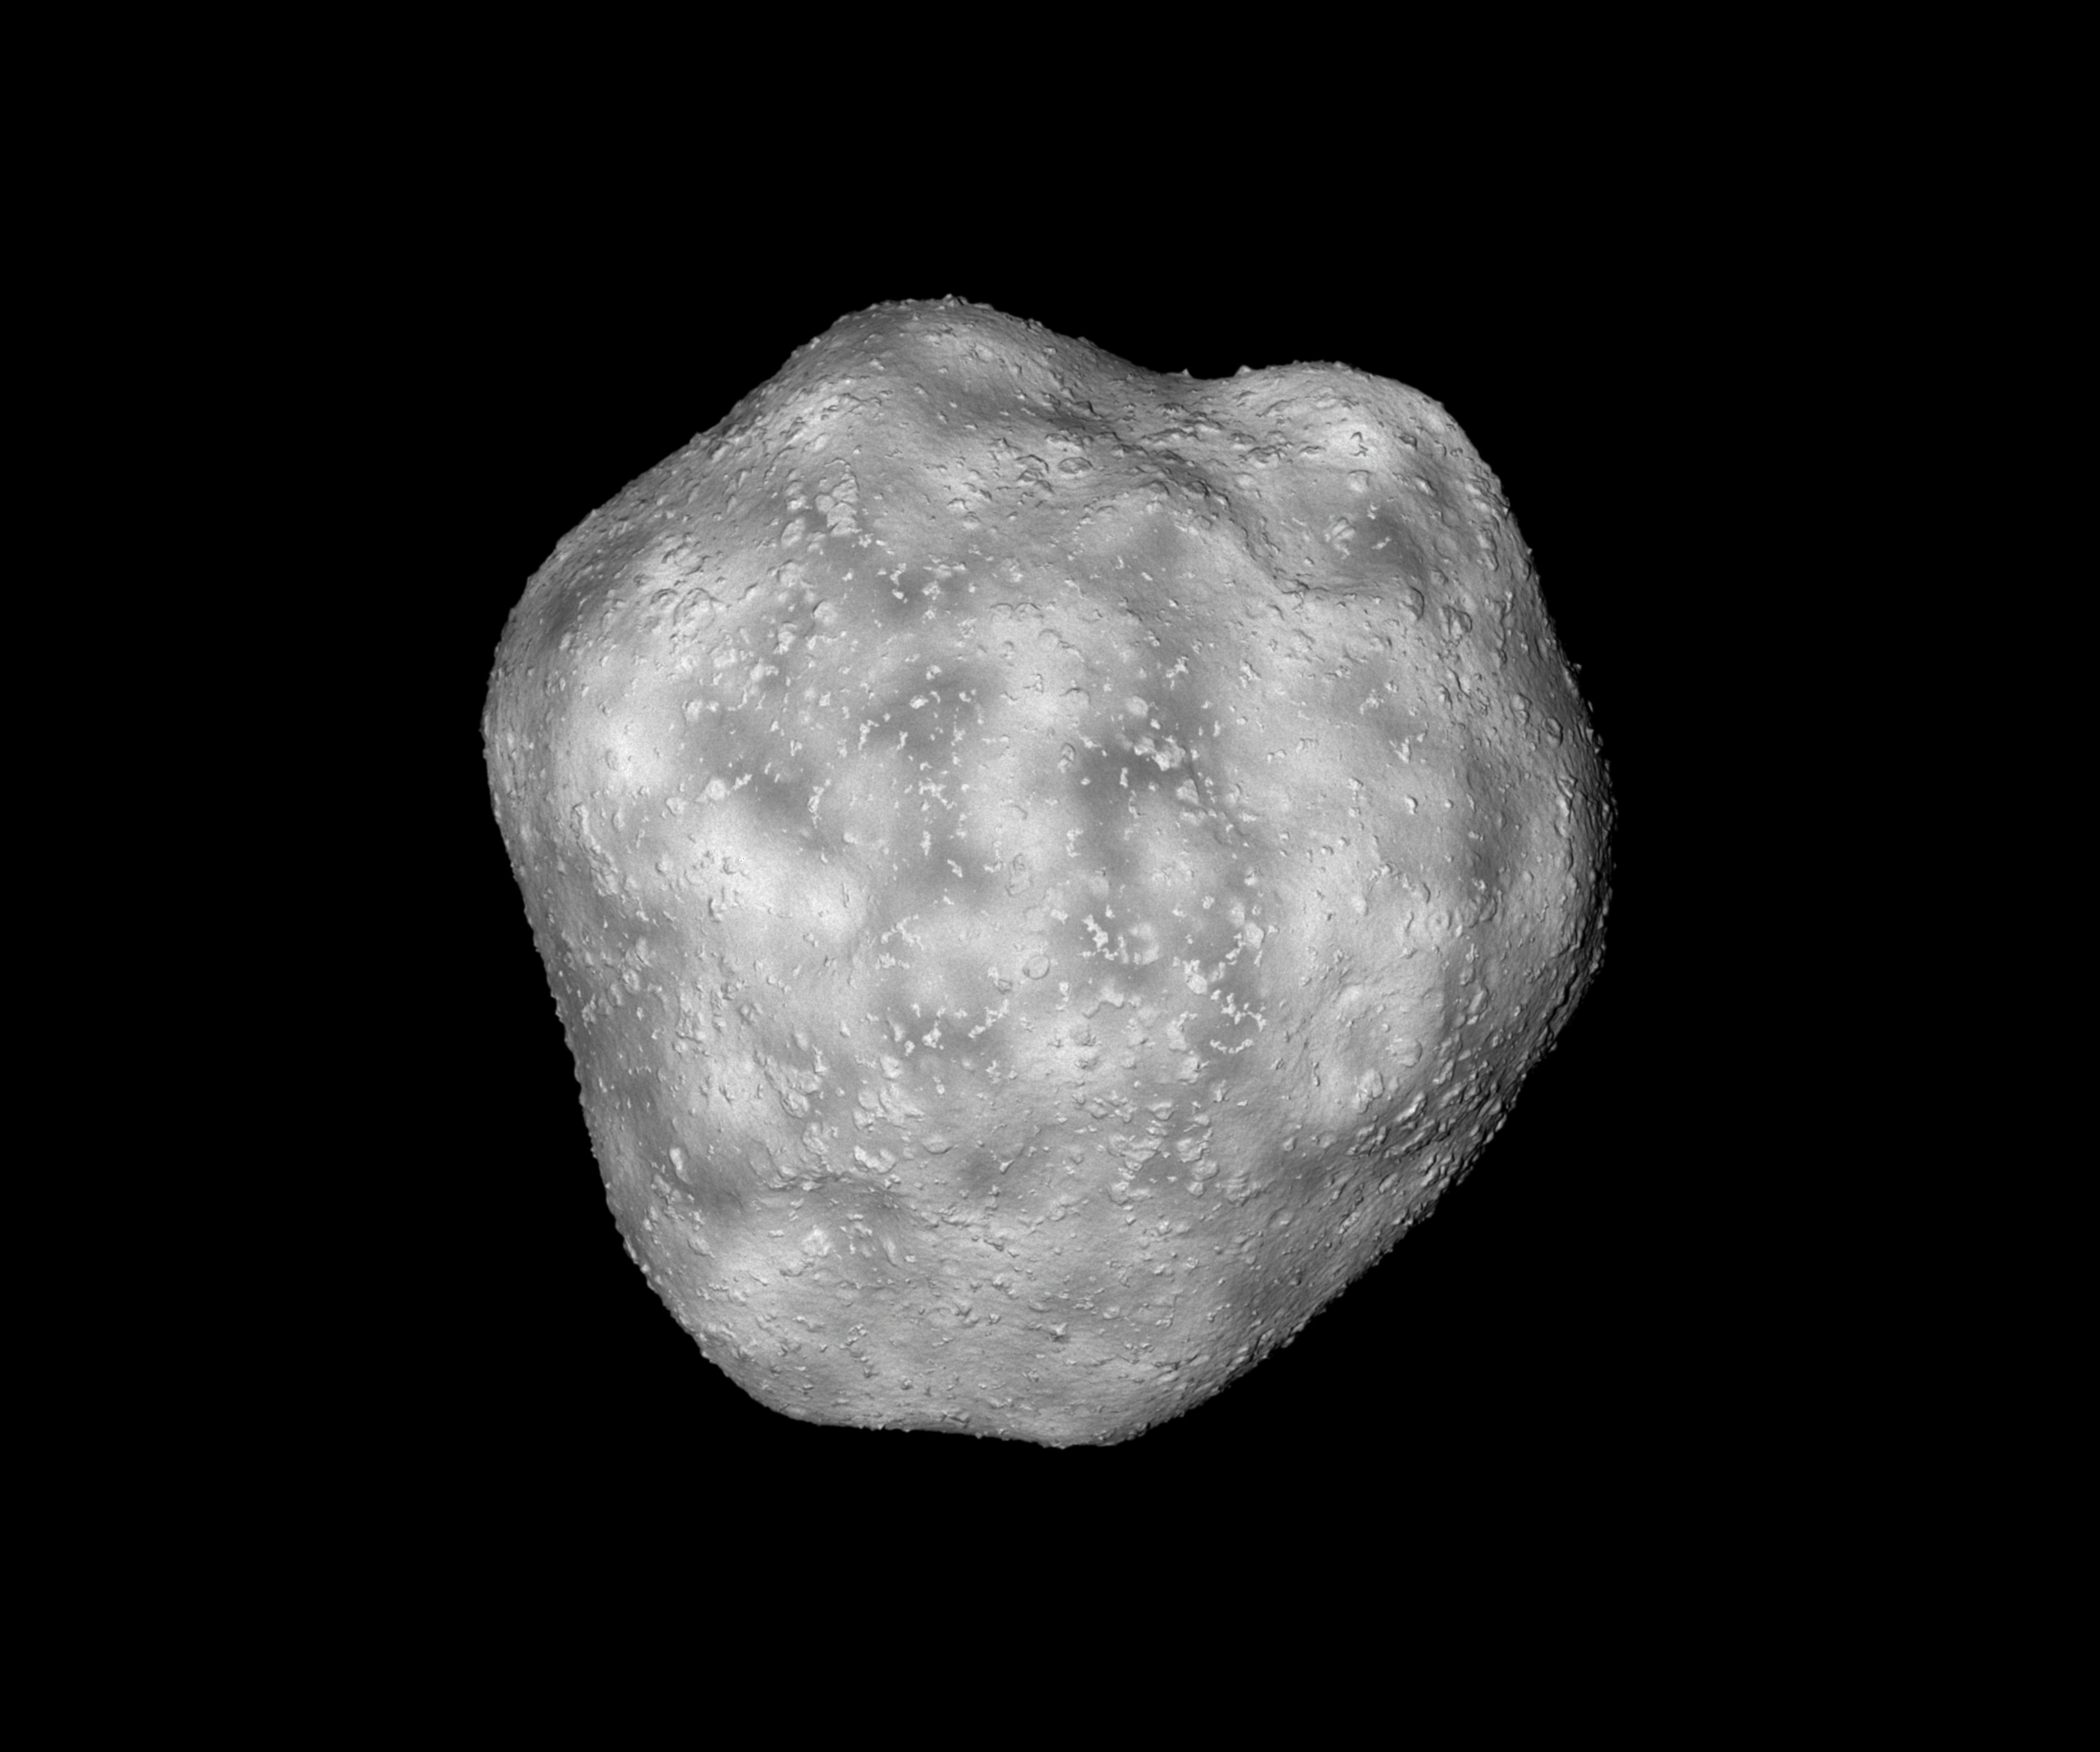
\includegraphics[width=\textwidth]{doc/thesis/0_figures/compare_quality/set1/jp2_100}
        \caption{}
        \label{fig:img_quality_comp_jp2_100_orig}
    \end{subfigure}
    \begin{subfigure}[b]{0.48\textwidth}
        \centering
        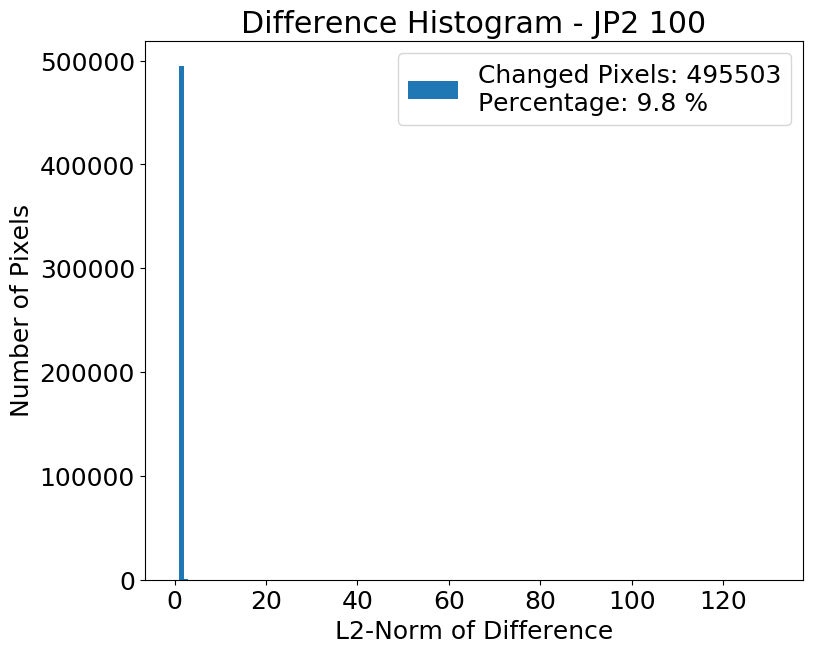
\includegraphics[width=\textwidth]{doc/thesis/0_figures/compare_quality/set1/jp2_100_diff_histogram}
        \caption{}
        \label{fig:img_quality_comp_jp2_100_histo}
    \end{subfigure}
    \\
    \begin{subfigure}[b]{0.48\textwidth}
        \centering
        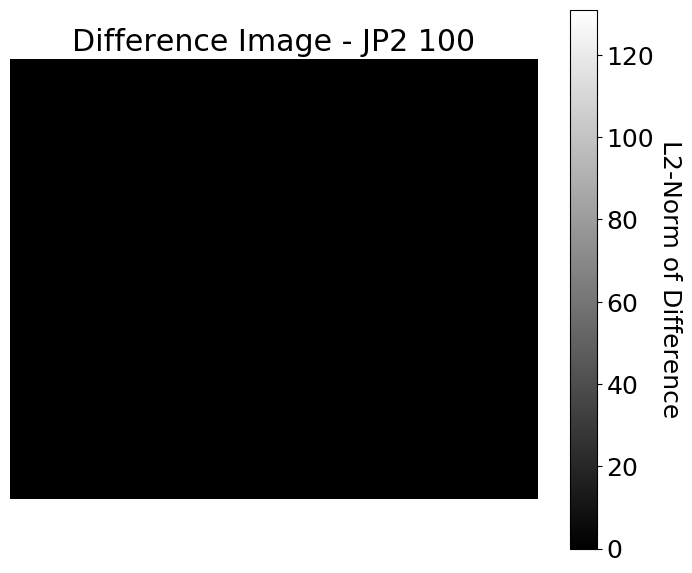
\includegraphics[width=\textwidth]{doc/thesis/0_figures/compare_quality/set1/jp2_100_diff_heatmap}
        \caption{}
        \label{fig:img_quality_comp_jp2_100_diff}
    \end{subfigure}
    \begin{subfigure}[b]{0.48\textwidth}
        \centering
        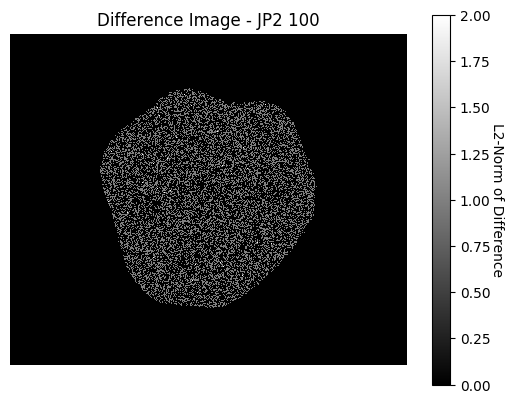
\includegraphics[width=\textwidth]{doc/thesis/0_figures/compare_quality/set1/jp2_100_diff_heatmap_rel}
        \caption{}
        \label{fig:img_quality_comp_jp2_100_diff_rel}
    \end{subfigure}
    \caption{Overall rendered image after compression with \gls{jp2} quality level 100. The L2-norm is applied to the difference between the greyscale images of the lossless and respective lossy image. (a) Image after lossy compression. (b) Histogram of L2-norms of differences. (c) L2-norm difference image with a colour scale from $0$ to $131$ for comparison between various compression levels. (d) L2-norm difference image with a colour scale from $0$ to the maximum L2-norm value for better visibility of compression effects.}
    \label{fig:img_quality_comp_jp2_100}
\end{figure}

\begin{figure}[htb]
    \centering
    \begin{subfigure}[b]{0.48\textwidth}
        \centering
        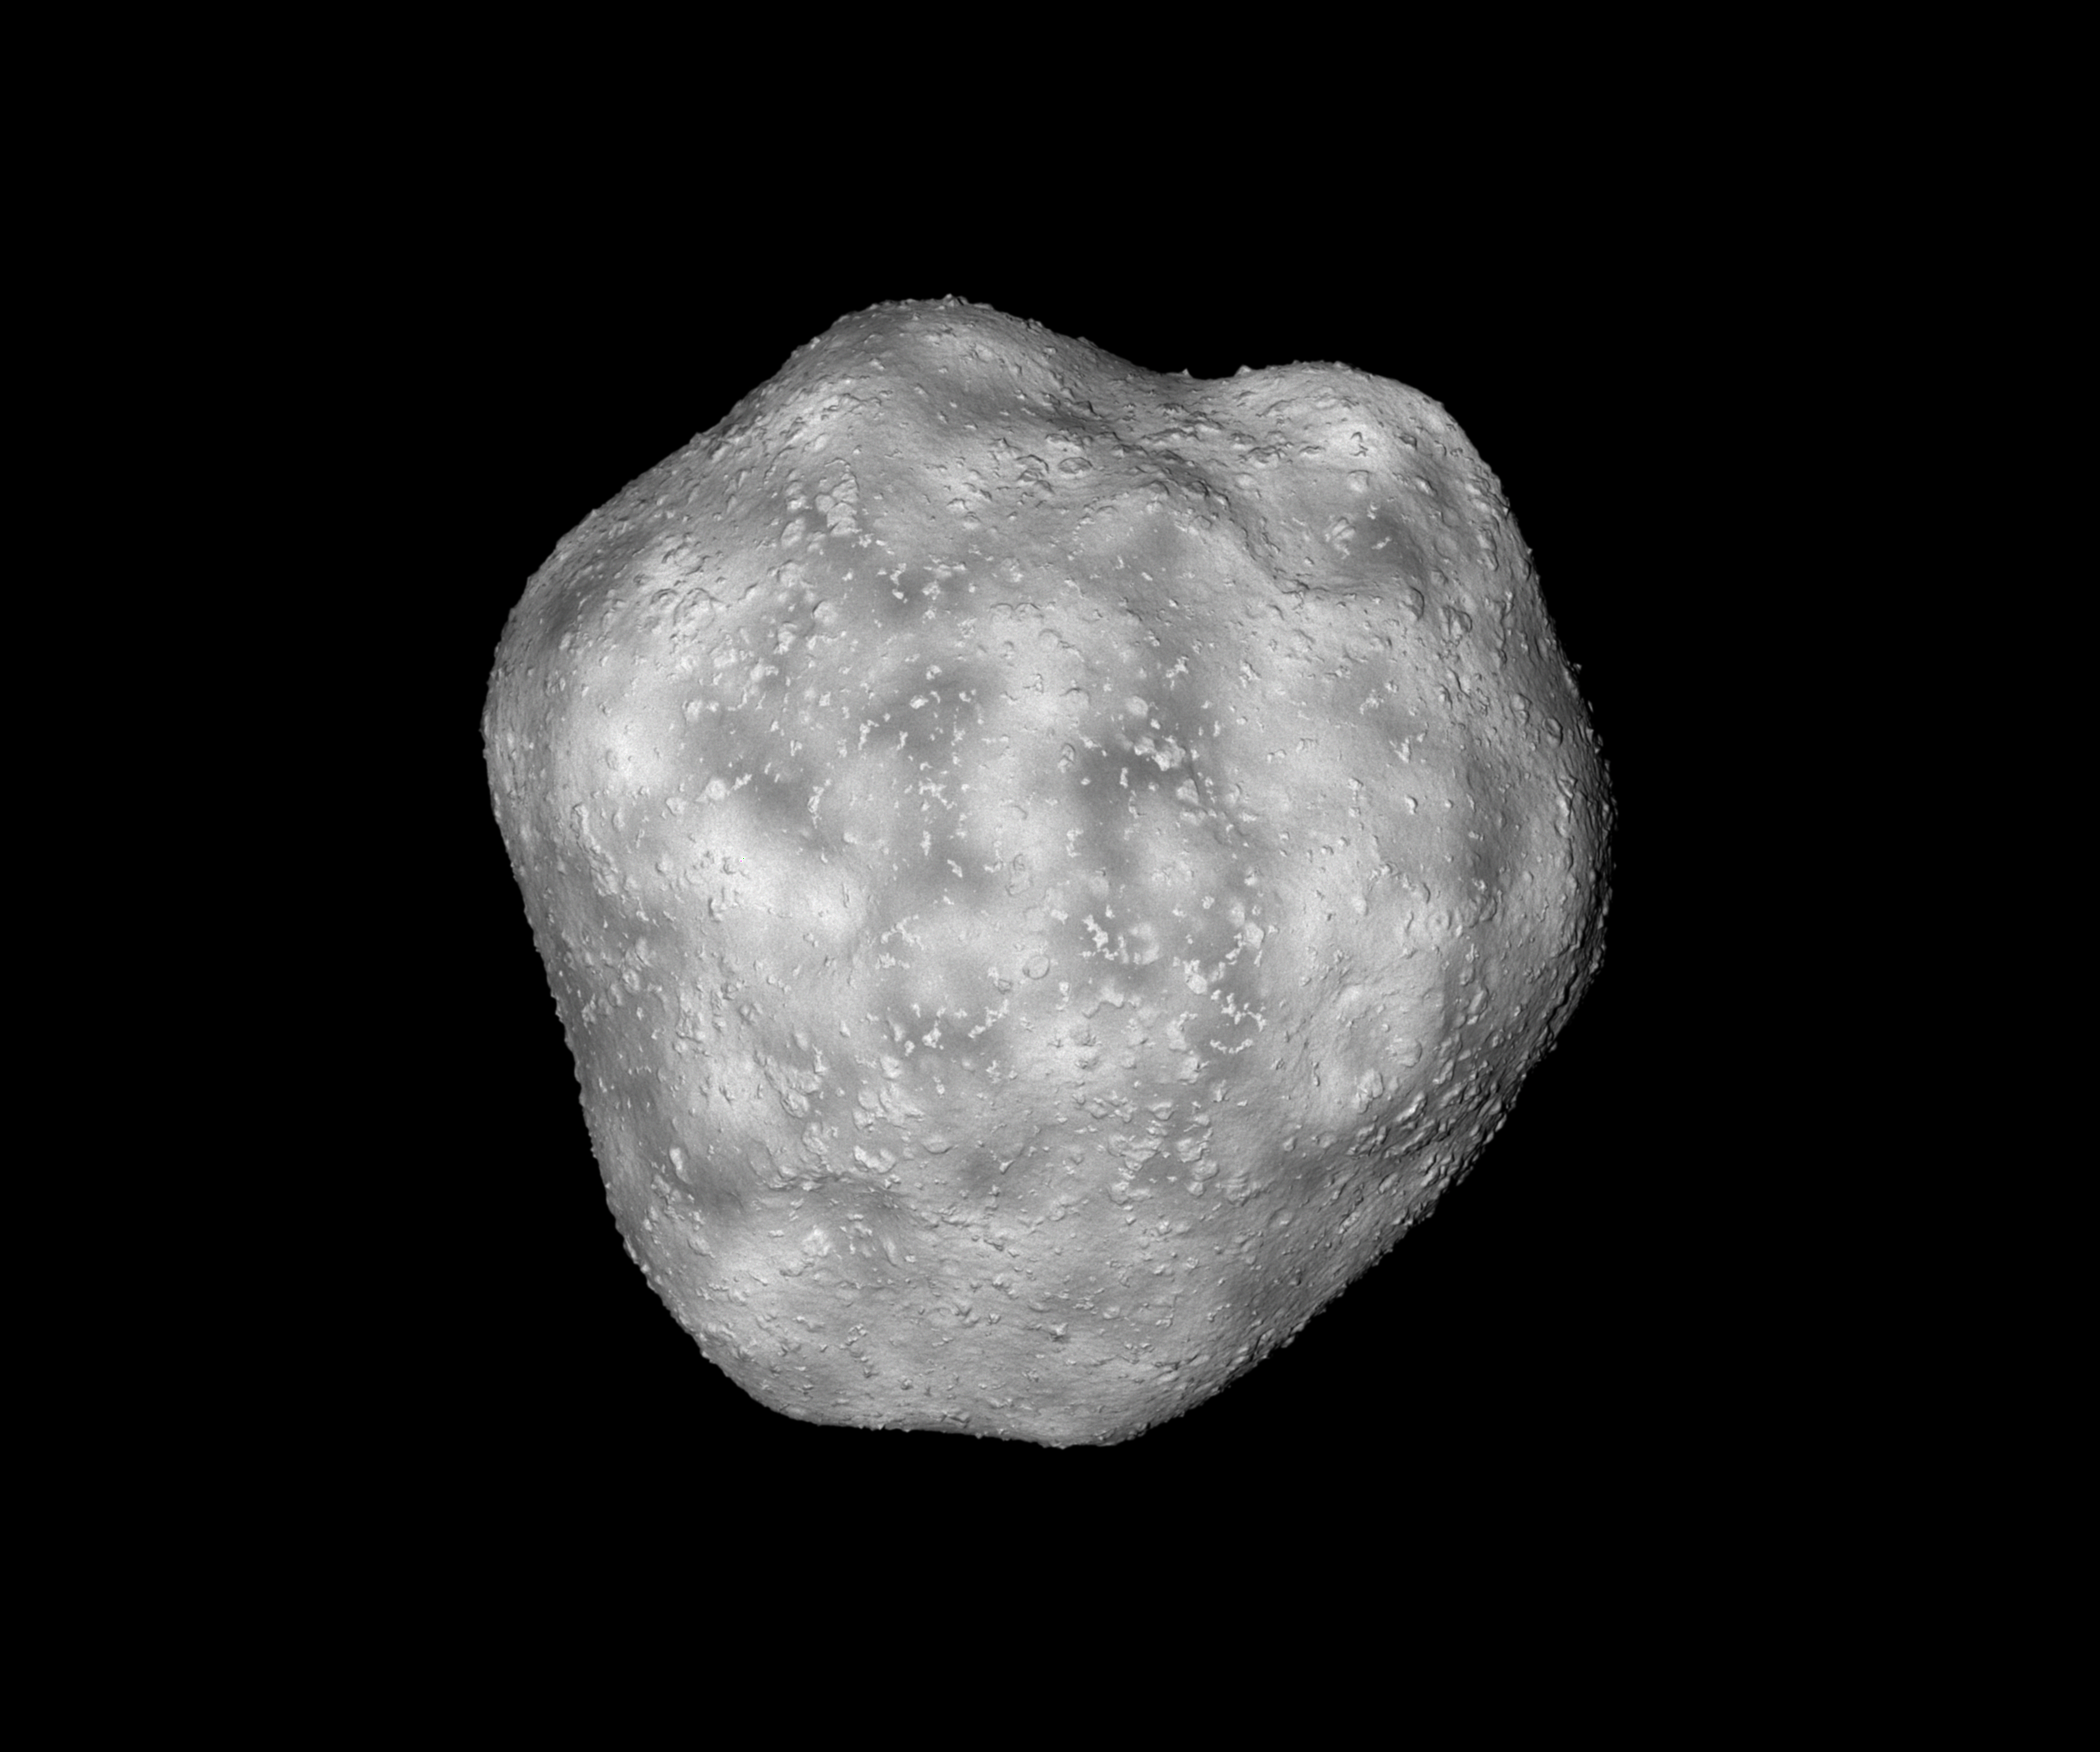
\includegraphics[width=\textwidth]{doc/thesis/0_figures/compare_quality/set1/jp2_1000}
        \caption{}
        \label{fig:img_quality_comp_jp2_1000_orig}
    \end{subfigure}
    \begin{subfigure}[b]{0.48\textwidth}
        \centering
        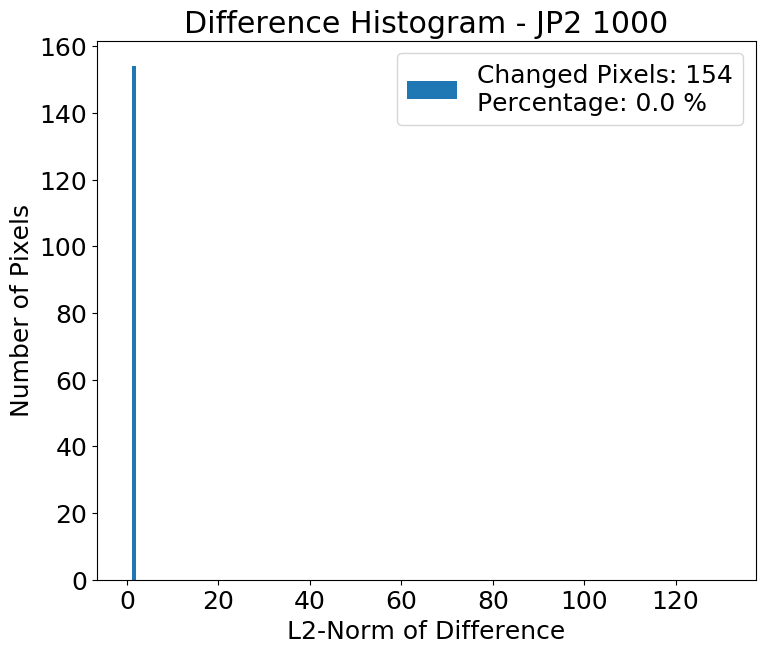
\includegraphics[width=\textwidth]{doc/thesis/0_figures/compare_quality/set1/jp2_1000_diff_histogram}
        \caption{}
        \label{fig:img_quality_comp_jp2_1000_histo}
    \end{subfigure}
    \\
    \begin{subfigure}[b]{0.48\textwidth}
        \centering
        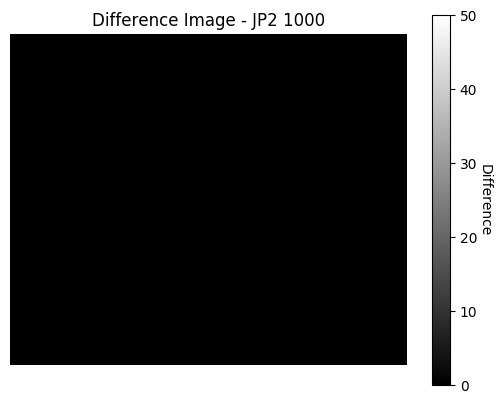
\includegraphics[width=\textwidth]{doc/thesis/0_figures/compare_quality/set1/jp2_1000_diff_heatmap}
        \caption{}
        \label{fig:img_quality_comp_jp2_1000_diff}
    \end{subfigure}
    \begin{subfigure}[b]{0.48\textwidth}
        \centering
        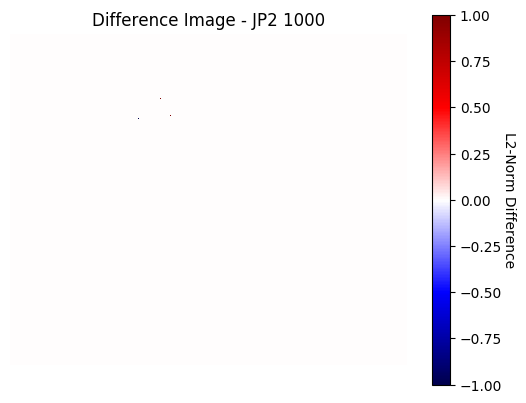
\includegraphics[width=\textwidth]{doc/thesis/0_figures/compare_quality/set1/jp2_1000_diff_heatmap_rel}
        \caption{}
        \label{fig:img_quality_comp_jp2_1000_diff_rel}
    \end{subfigure}
    \caption{Overall rendered image after compression with \gls{jp2} quality level 1000. The L2-norm is applied to the difference between the greyscale images of the lossless and respective lossy image. (a) Image after lossy compression. (b) Histogram of L2-norms of differences. (c) L2-norm difference image with a colour scale from $0$ to $131$ for comparison between various compression levels. (d) L2-norm difference image with a colour scale from $0$ to the maximum L2-norm value for better visibility of compression effects.}
    \label{fig:img_quality_comp_jp2_1000}
\end{figure}
\clearpage
Overall images show that lossy compression introduces artefacts for all quality levels. Visual inspection of the rendered images does not reveal many changes between different quality levels. However, histograms reveal that the number of altered pixels and the amount of alteration increases with decreasing quality level. The difference image for quality level 1000 in Figure~\ref{fig:img_quality_comp_jp2_1000_diff_rel} shows the minute changes from compression. The difference images in Figures~\ref{fig:img_quality_comp_jp2_1_diff_rel},~\ref{fig:img_quality_comp_jp2_5_diff_rel},~\ref{fig:img_quality_comp_jp2_10_diff_rel}~and~\ref{fig:img_quality_comp_jp2_100_diff_rel} outline the shape of the \gls{sssb} hence compression artefacts are spread across the entire \gls{sssb}. Comparing the difference images in Figures~\ref{fig:img_quality_comp_jp2_1_diff},~\ref{fig:img_quality_comp_jp2_5_diff},~\ref{fig:img_quality_comp_jp2_10_diff},~\ref{fig:img_quality_comp_jp2_100_diff}~and~\ref{fig:img_quality_comp_jp2_1000_diff} which use the same scale for all quality levels show that the alteration in quality levels \SI{100}{} and \SI{1000}{} are much lower compared to quality levels \SI{1}{}, \SI{5}{} and \SI{10}{}.

Figures~\ref{fig:img_quality_comp_jp2_1_center} to \ref{fig:img_quality_comp_jp2_1000_center} show compressed close-up images, difference histograms and difference images after compression with \gls{jp2} with quality levels \SI{1}{}, \SI{5}{}, \SI{10}{}, \SI{100}{} and \SI{1000}{}.

Comparing the close-up images of various quality levels in Figures~\ref{fig:img_quality_comp_jp2_1_center_orig},~\ref{fig:img_quality_comp_jp2_5_center_orig},~\ref{fig:img_quality_comp_jp2_10_center_orig},~\ref{fig:img_quality_comp_jp2_100_center_orig} and~\ref{fig:img_quality_comp_jp2_1000_center_orig} reveals a degradation of image quality with decreasing compression quality levels. Histograms confirm that the number of altered pixels and the amount of alteration increases with decreasing quality level. The difference image for quality level 1000 in Figure~\ref{fig:img_quality_comp_jp2_1000_center_diff_rel} and the respective histogram show that there were no altered pixels for quality level 1000, i.e. compression was lossless. The difference image in Figure~\ref{fig:img_quality_comp_jp2_100_center_diff_rel} resembles random noise. In contrast, difference images in Figures~\ref{fig:img_quality_comp_jp2_1_center_diff_rel},~\ref{fig:img_quality_comp_jp2_5_center_diff_rel} and~\ref{fig:img_quality_comp_jp2_10_center_diff_rel} show non-random artefacts correlated with surface features when comparing to the unaltered image in Figure~\ref{fig:img_quality_comp_jp2_1000_center_orig}. However, when comparing the difference images in Figures~\ref{fig:img_quality_comp_jp2_1_center_diff}, \ref{fig:img_quality_comp_jp2_5_center_diff}, \ref{fig:img_quality_comp_jp2_10_center_diff}, \ref{fig:img_quality_comp_jp2_100_center_diff} and \ref{fig:img_quality_comp_jp2_1000_center_diff} which use the same scale for all quality levels, we see the alteration in quality levels \SI{100}{} and \SI{1000}{} are much lower compared to quality levels \SI{1}{}, \SI{5}{} and \SI{10}{}.

Comparing results of the overall images with results of the close-up images reveals that overall images are less altered by compression relative to their size. A substantial portion of overall images is covered by a black background thus compression does change less pixels than in close-up images. Overall difference images resemble random noise. In contrast, close-up images reveal a relation between surface features and compression artefacts for low quality levels.

\begin{figure}[htb]
    \centering
    \begin{subfigure}[b]{0.48\textwidth}
        \centering
        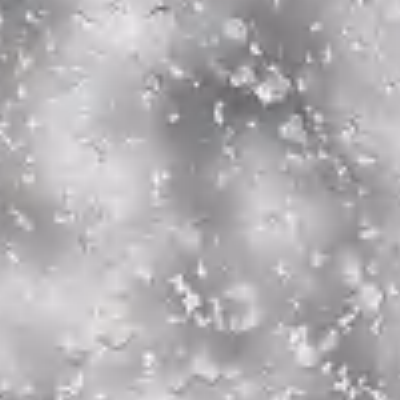
\includegraphics[width=\textwidth]{doc/thesis/0_figures/compare_quality/set1/jp2_1_center}
        \caption{}
        \label{fig:img_quality_comp_jp2_1_center_orig}
    \end{subfigure}
    \begin{subfigure}[b]{0.48\textwidth}
        \centering
        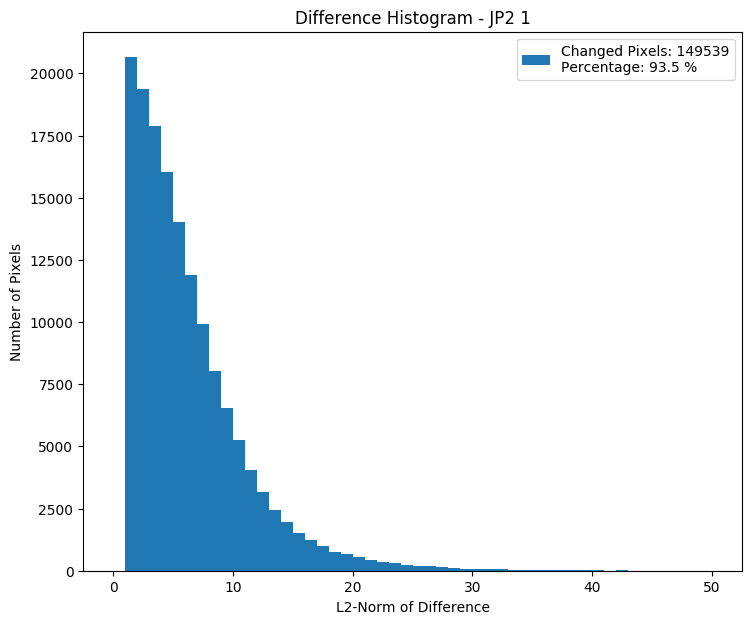
\includegraphics[width=\textwidth]{doc/thesis/0_figures/compare_quality/set1/jp2_1_center_diff_histogram}
        \caption{}
        \label{fig:img_quality_comp_jp2_1_center_histo}
    \end{subfigure}
    \\
    \begin{subfigure}[b]{0.48\textwidth}
        \centering
        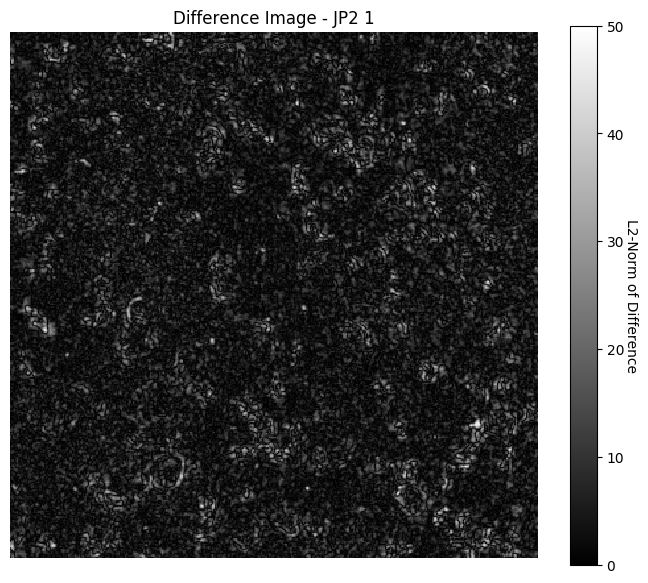
\includegraphics[width=\textwidth]{doc/thesis/0_figures/compare_quality/set1/jp2_1_center_diff_heatmap}
        \caption{}
        \label{fig:img_quality_comp_jp2_1_center_diff}
    \end{subfigure}
    \begin{subfigure}[b]{0.48\textwidth}
        \centering
        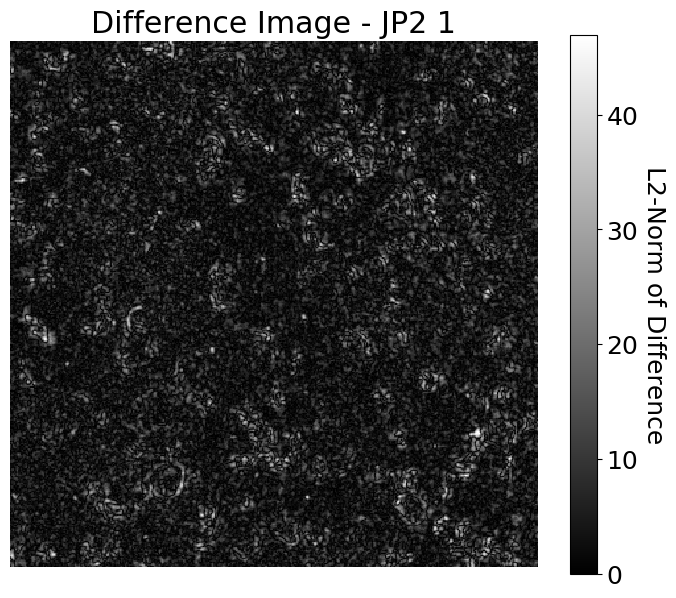
\includegraphics[width=\textwidth]{doc/thesis/0_figures/compare_quality/set1/jp2_1_center_diff_heatmap_rel}
        \caption{}
        \label{fig:img_quality_comp_jp2_1_center_diff_rel}
    \end{subfigure}
    \caption{Close-up rendered image after compression with \gls{jp2} quality level 1. The L2-norm is applied to the difference between the greyscale images of the lossless and respective lossy image. (a) Image after lossy compression. (b) Histogram of L2-norms of differences. (c) L2-norm difference image with a colour scale from $0$ to $51$ for comparison between various compression levels. (d) L2-norm difference image with a colour scale from $0$ to the maximum L2-norm value for better visibility of compression effects.}
    \label{fig:img_quality_comp_jp2_1_center}
\end{figure}

\begin{figure}[htb]
    \centering
    \begin{subfigure}[b]{0.48\textwidth}
        \centering
        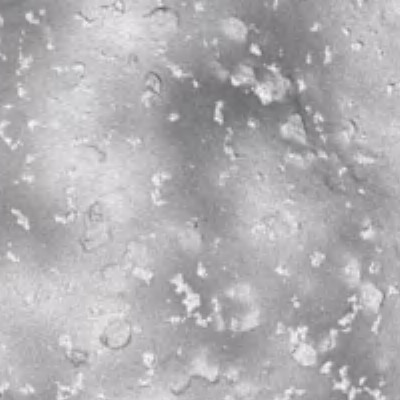
\includegraphics[width=\textwidth]{doc/thesis/0_figures/compare_quality/set1/jp2_5_center}
        \caption{}
        \label{fig:img_quality_comp_jp2_5_center_orig}
    \end{subfigure}
    \begin{subfigure}[b]{0.48\textwidth}
        \centering
        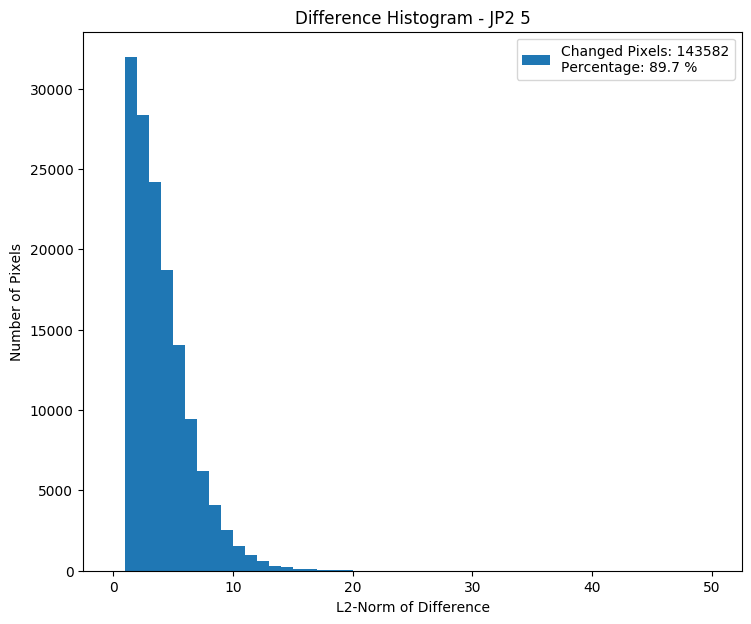
\includegraphics[width=\textwidth]{doc/thesis/0_figures/compare_quality/set1/jp2_5_center_diff_histogram}
        \caption{}
        \label{fig:img_quality_comp_jp2_5_center_histo}
    \end{subfigure}
    \\
    \begin{subfigure}[b]{0.48\textwidth}
        \centering
        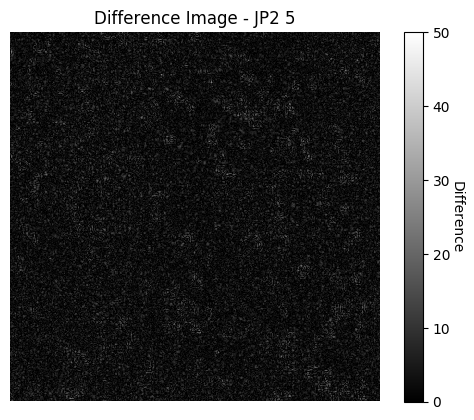
\includegraphics[width=\textwidth]{doc/thesis/0_figures/compare_quality/set1/jp2_5_center_diff_heatmap}
        \caption{}
        \label{fig:img_quality_comp_jp2_5_center_diff}
    \end{subfigure}
    \begin{subfigure}[b]{0.48\textwidth}
        \centering
        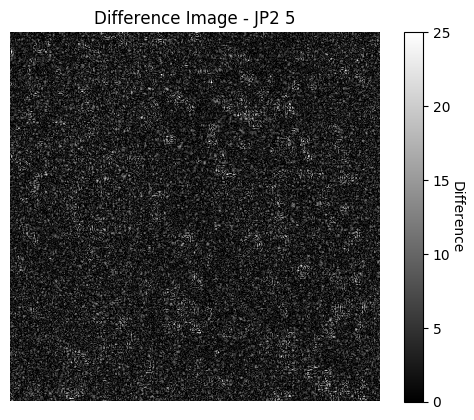
\includegraphics[width=\textwidth]{doc/thesis/0_figures/compare_quality/set1/jp2_5_center_diff_heatmap_rel}
        \caption{}
        \label{fig:img_quality_comp_jp2_5_center_diff_rel}
    \end{subfigure}
    \caption{Close-up rendered image after compression with \gls{jp2} quality level 5. The L2-norm is applied to the difference between the greyscale images of the lossless and respective lossy image. (a) Image after lossy compression. (b) Histogram of L2-norms of differences. (c) L2-norm difference image with a colour scale from $0$ to $51$ for comparison between various compression levels. (d) L2-norm difference image with a colour scale from $0$ to the maximum L2-norm value for better visibility of compression effects.}
    \label{fig:img_quality_comp_jp2_5_center}
\end{figure}

\begin{figure}[htb]
    \centering
    \begin{subfigure}[b]{0.48\textwidth}
        \centering
        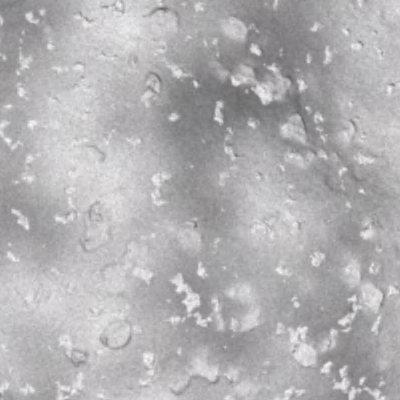
\includegraphics[width=\textwidth]{doc/thesis/0_figures/compare_quality/set1/jp2_10_center}
        \caption{}
        \label{fig:img_quality_comp_jp2_10_center_orig}
    \end{subfigure}
    \begin{subfigure}[b]{0.48\textwidth}
        \centering
        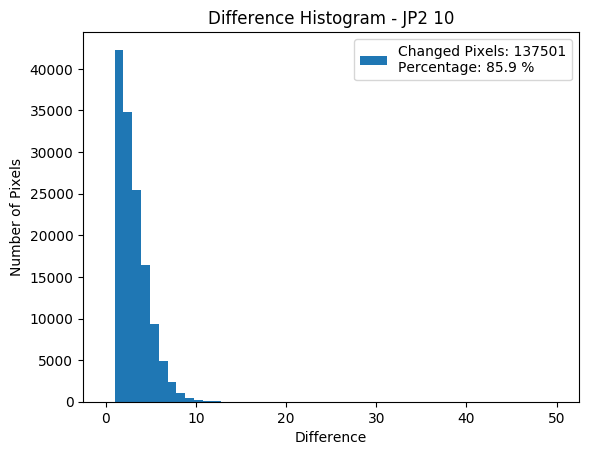
\includegraphics[width=\textwidth]{doc/thesis/0_figures/compare_quality/set1/jp2_10_center_diff_histogram}
        \caption{}
        \label{fig:img_quality_comp_jp2_10_center_histo}
    \end{subfigure}
    \\
    \begin{subfigure}[b]{0.48\textwidth}
        \centering
        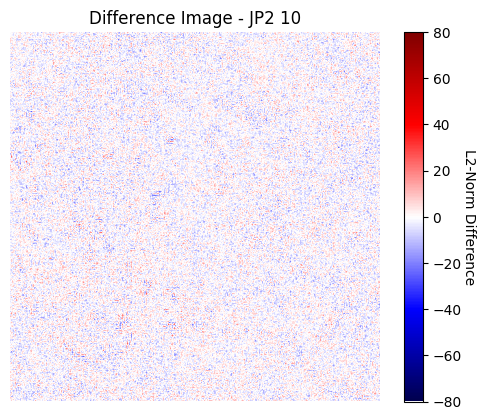
\includegraphics[width=\textwidth]{doc/thesis/0_figures/compare_quality/set1/jp2_10_center_diff_heatmap}
        \caption{}
        \label{fig:img_quality_comp_jp2_10_center_diff}
    \end{subfigure}
    \begin{subfigure}[b]{0.48\textwidth}
        \centering
        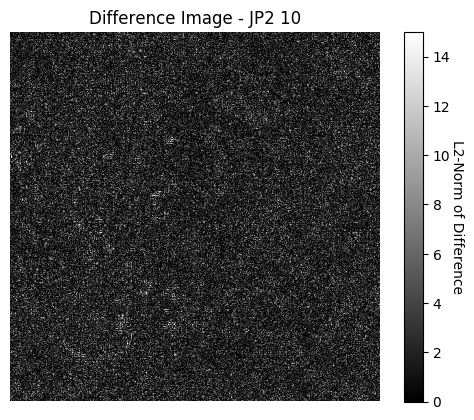
\includegraphics[width=\textwidth]{doc/thesis/0_figures/compare_quality/set1/jp2_10_center_diff_heatmap_rel}
        \caption{}
        \label{fig:img_quality_comp_jp2_10_center_diff_rel}
    \end{subfigure}
    \caption{Close-up rendered image after compression with \gls{jp2} quality level 10. The L2-norm is applied to the difference between the greyscale images of the lossless and respective lossy image. (a) Image after lossy compression. (b) Histogram of L2-norms of differences. (c) L2-norm difference image with a colour scale from $0$ to $51$ for comparison between various compression levels. (d) L2-norm difference image with a colour scale from $0$ to the maximum L2-norm value for better visibility of compression effects.}
    \label{fig:img_quality_comp_jp2_10_center}
\end{figure}

\begin{figure}[htb]
    \centering
    \begin{subfigure}[b]{0.48\textwidth}
        \centering
        \includegraphics[width=\textwidth]{doc/thesis/0_figures/compare_quality/set1/jp2_100_center}
        \caption{}
        \label{fig:img_quality_comp_jp2_100_center_orig}
    \end{subfigure}
    \begin{subfigure}[b]{0.48\textwidth}
        \centering
        \includegraphics[width=\textwidth]{doc/thesis/0_figures/compare_quality/set1/jp2_100_center_diff_histogram}
        \caption{}
        \label{fig:img_quality_comp_jp2_100_center_histo}
    \end{subfigure}
    \\
    \begin{subfigure}[b]{0.48\textwidth}
        \centering
        \includegraphics[width=\textwidth]{doc/thesis/0_figures/compare_quality/set1/jp2_100_center_diff_heatmap}
        \caption{}
        \label{fig:img_quality_comp_jp2_100_center_diff}
    \end{subfigure}
    \begin{subfigure}[b]{0.48\textwidth}
        \centering
        \includegraphics[width=\textwidth]{doc/thesis/0_figures/compare_quality/set1/jp2_100_center_diff_heatmap_rel}
        \caption{}
        \label{fig:img_quality_comp_jp2_100_center_diff_rel}
    \end{subfigure}
    \caption{Close-up rendered image after compression with \gls{jp2} quality level 100. The L2-norm is applied to the difference between the greyscale images of the lossless and respective lossy image. (a) Image after lossy compression. (b) Histogram of L2-norms of differences. (c) L2-norm difference image with a colour scale from $0$ to $51$ for comparison between various compression levels. (d) L2-norm difference image with a colour scale from $0$ to the maximum L2-norm value for better visibility of compression effects.}
    \label{fig:img_quality_comp_jp2_100_center}
\end{figure}

\begin{figure}[htb]
    \centering
    \begin{subfigure}[b]{0.48\textwidth}
        \centering
        \includegraphics[width=\textwidth]{doc/thesis/0_figures/compare_quality/set1/jp2_1000_center}
        \caption{}
        \label{fig:img_quality_comp_jp2_1000_center_orig}
    \end{subfigure}
    \begin{subfigure}[b]{0.48\textwidth}
        \centering
        \includegraphics[width=\textwidth]{doc/thesis/0_figures/compare_quality/set1/jp2_1000_center_diff_histogram}
        \caption{}
        \label{fig:img_quality_comp_jp2_1000_center_histo}
    \end{subfigure}
    \\
    \begin{subfigure}[b]{0.48\textwidth}
        \centering
        \includegraphics[width=\textwidth]{doc/thesis/0_figures/compare_quality/set1/jp2_1000_center_diff_heatmap}
        \caption{}
        \label{fig:img_quality_comp_jp2_1000_center_diff}
    \end{subfigure}
    \begin{subfigure}[b]{0.48\textwidth}
        \centering
        \includegraphics[width=\textwidth]{doc/thesis/0_figures/compare_quality/set1/jp2_1000_center_diff_heatmap_rel}
        \caption{}
        \label{fig:img_quality_comp_jp2_1000_center_diff_rel}
    \end{subfigure}
    \caption{Close-up rendered image after compression with \gls{jp2} quality level 1000. The L2-norm is applied to the difference between the greyscale images of the lossless and respective lossy image. (a) Image after lossy compression. (b) Histogram of L2-norms of differences. (c) L2-norm difference image with a colour scale from $0$ to $51$ for comparison between various compression levels. (d) L2-norm difference image with a colour scale from $0$ to the maximum L2-norm value for better visibility of compression effects.}
    \label{fig:img_quality_comp_jp2_1000_center}
\end{figure}

\clearpage

\subsection{Reconstruction}
\gls{sispo} reconstruction used the parameters given in Table~\ref{tab:comp_settings}. refine\_options is set to NONE to increase the probability of the \gls{sfm} algorithms to converge. Camera calibration as described in Section~\ref{sec:t_cv} is not required since intrinsic camera parameters can be determined with sufficient accuracy before launch in space missions hence the parameters do not need to be optimised.

\begin{table}[htb]
    \centering
    \caption{Reconstruction Settings}
    \label{tab:comp_settings}
    \begin{tabular}{l|l}
        \textbf{Parameter Name} & \textbf{Value} \\ \hline
        export\_type       & obj   \\
        focal & 66667 \\
        cam\_model & \SI{1}{}     \\
        geo\_model & \SI{10}{\kilo\meter\per\second} \\
        num\_overlaps  & \SI{4}{} \\
        use\_prior & \SI{1}{} \\
        use\_upright & \SI{0}{} \\
        force\_compute & \SI{0}{} \\
        descriptor & SIFT \\
        d\_preset & ULTRA \\
        method & FASTCASCADEHASHINGL2 \\
        refine\_options & NONE \\
        reduce\_memory & 1
    \end{tabular}
\end{table}

\subsubsection{Reconstructed Model Comparison}
Reconstruction was successful in all cases presented in Table~\ref{tab:sim_params} except for a \SI{400}{\kilo\meter} fly-by of a \SI{1}{\kilo\meter} nucleus and the lowest compression quality level. The number of reconstructed points decreases with decreasing \gls{sssb} size and an increasing closest distance, i.e. with decreasing visible size in the images.

The number of points in the densified point cloud ranges from approximately \SI{6e6}{} for a \SI{50}{\kilo\meter} fly-by of a \SI{10}{\kilo\meter} \gls{sssb} to approximately \SI{2e3}{} for a \SI{400}{\kilo\meter} fly-by of a \SI{1}{\kilo\meter} \gls{sssb}. These two fly-by scenarios represent the two boundary cases of the simulation results, these are compared in more detail. The quality of other reconstructed \gls{3d} models is in between the presented results and are therefore not analysed further.

A comparison of the point clouds and resulting meshes of the two scenarios is shown in Figure~\ref{fig:points_models_comp}. The large variation in points between Figure~\ref{fig:points_50_10}~and~\ref{fig:points_400_1} after reconstruction and densification strongly influences \gls{3d} model quality. Both point clouds contain visible outliers which are removed in the \gls{3d} models.
\begin{figure}[htb]
    \centering
        \begin{subfigure}[b]{0.42\textwidth}
            \centering
            \includegraphics[width=\textwidth,height=6.2cm]{doc/thesis/0_figures/models_quality/50_10/120_50_10_dense2.png}
            \caption{}
            \label{fig:points_50_10}
        \end{subfigure}
        \begin{subfigure}[b]{0.42\textwidth}
            \centering
            \includegraphics[width=\textwidth,height=6.2cm]{doc/thesis/0_figures/models_quality/400_1/120_400_1_points2.png}
            \caption{}
            \label{fig:points_400_1}
        \end{subfigure}
        \\
        \begin{subfigure}[b]{0.42\textwidth}
            \centering
            \includegraphics[width=\textwidth,height=6.2cm]{doc/thesis/0_figures/models_quality/50_10/120_50_10_refine2.png}
            \caption{} %1072422
            \label{fig:models_50_10}
        \end{subfigure}
        \begin{subfigure}[b]{0.42\textwidth}
            \centering
            \includegraphics[width=\textwidth,height=6.2cm]{doc/thesis/0_figures/models_quality/400_1/120_400_1_mesh2.png}
            \caption{}
            \label{fig:models_400_1}
        \end{subfigure}
    \caption{Images showing point clouds and resulting \gls{3d} models of two fly-by scenarios representing boundary cases with successful reconstructions. (a)~Point cloud with $\approx\SI{6e6}{}$~points representing a \SI{10}{\kilo\meter} \gls{sssb} after a \SI{50}{\kilo\meter} fly-by. (b)~Point cloud with $\approx\SI{2e3}{}$~points representing a \SI{1}{\kilo\meter} \gls{sssb} after a \SI{400}{\kilo\meter} fly-by. Point cloud densification failed for in this fly-by scenario, therefore the sparse point cloud is depicted. (c)~Mesh based on the point cloud in~(a) with $\approx\SI{1e6}{}$~vertices. (d)~Mesh based on the point cloud in~(b) with $\approx\SI{700}{}$~vertices. Mesh refinement failed in this scenario, therefore the sparse mesh is depicted.}
    \label{fig:points_models_comp}
\end{figure}

Texturing only alters the appearance of a \gls{3d} model but not its quality thus meshes after refinement are compared. Comparing the \gls{3d} models in Figures~\ref{fig:models_50_10}~and~\ref{fig:models_400_1} shows the influence of the number of points on the \gls{3d} models. Single vertices of the model in Figure~\ref{fig:models_400_1} are visible. In contrast, the more detailed model in Figure~\ref{fig:models_50_10} represents detailed surface features such as boulders.

% \begin{figure}[H]
%     \centering

%     \caption{Images showing \gls{3d} models reconstructed from the point clouds shown in Figure~\ref{fig:points_dense_comp}. }
%     \label{fig:models_comp}
% \end{figure}

\subsubsection{Compression Effects on Reconstructed 3D Models}
The quality of  reconstructed \gls{3d} models is compared numerically. The number of points after densification, the number of vertices and the number of faces of the refined meshed model are compared for different levels of compression for the same simulation scenario. The number of points, vertices and faces relate to the level of detail of a \gls{3d} model. Moreover, the number of points in relation to the number of vertices can be used to analyse the amount of outliers in the point cloud since outlier points cannot be included into a meaningful \gls{3d} model. Values are normalised to the results of \gls{png} to compare lossless compression against lossy compression.

The theoretical size of \SI{120}{} images is compared to the highest compression ratio of lossless compression using \gls{png}. A series of \SI{120}{}~\gls{rgb} images with $\SI{2454}{} \times \SI{2054}{}$~pixels and a colour depth of \SI{8}{\bit} has a data size of \gls{d_s}$ = 120 \times 2454 \times 2054 \times 3 \times \SI{8}{\bit} = \SI{1814.6}{\mega\byte}$. The \gls{png} data sets have sizes ranging from \SI{5.2}{\mega\byte} to \SI{564.6}{\mega\byte}, i.e. \SI{0.3}{\percent} to \SI{31.1}{\percent} of the raw data size. Varying apparent sizes of the nucleus and the resulting varying black portion of an image explain the varying and high possible compression ratios of \gls{png}.
% 564573825 / 5172917; 1814585760

Figure~\ref{fig:recon_stats_1} and Figure~\ref{fig:recon_stats_10} compare effects of lossless compression using \gls{png} and varying quality levels of lossy compression using \gls{jp2}.

\begin{figure}[htb]
    \centering
        \begin{subfigure}[b]{0.49\textwidth}
            \centering
            \includegraphics[width=\textwidth]{doc/thesis/0_figures/recon/50km_1k}
            \caption{}
            \label{fig:recon_120_50_1}
        \end{subfigure}
        \begin{subfigure}[b]{0.49\textwidth}
            \centering
            \includegraphics[width=\textwidth]{doc/thesis/0_figures/recon/100km_1k}
            \caption{}
            \label{fig:recon_120_100_1}
        \end{subfigure}
        \\
        \begin{subfigure}[b]{0.49\textwidth}
            \centering
            \includegraphics[width=\textwidth]{doc/thesis/0_figures/recon/200km_1k}
            \caption{}
            \label{fig:recon_120_200_1}
        \end{subfigure}
        \begin{subfigure}[b]{0.49\textwidth}
            \centering
            \includegraphics[width=\textwidth]{doc/thesis/0_figures/recon/400km_1k}
            \caption{}
            \label{fig:recon_120_400_1}
        \end{subfigure}
    \caption{Comparison of reconstruction output after image compression with varying quality levels for a \SI{1}{\kilo\meter} \gls{sssb} with varying fly-by distances. (a) Fly-by distance \SI{50}{\kilo\meter}. (b) Fly-by distance \SI{100}{\kilo\meter}. (c) Fly-by distance \SI{200}{\kilo\meter}. (d) Fly-by distance \SI{400}{\kilo\meter}.}
    \label{fig:recon_stats_1}
\end{figure}

\begin{figure}[htb]
    \centering
        \begin{subfigure}[b]{0.49\textwidth}
            \centering
            \includegraphics[width=\textwidth]{doc/thesis/0_figures/recon/50km_10k}
            \caption{}
            \label{fig:recon_120_50_10}
        \end{subfigure}
        \begin{subfigure}[b]{0.49\textwidth}
            \centering
            \includegraphics[width=\textwidth]{doc/thesis/0_figures/recon/100km_10k}
            \caption{}
            \label{fig:recon_120_100_10}
        \end{subfigure}
        \\
        \begin{subfigure}[b]{0.49\textwidth}
            \centering
            \includegraphics[width=\textwidth]{doc/thesis/0_figures/recon/200km_10k}
            \caption{}
            \label{fig:recon_120_200_10}
        \end{subfigure}
        \begin{subfigure}[b]{0.49\textwidth}
            \centering
            \includegraphics[width=\textwidth]{doc/thesis/0_figures/recon/400km_10k}
            \caption{}
            \label{fig:recon_120_400_10}
        \end{subfigure}
    \caption{Comparison of reconstruction output after image compression with varying quality levels for a \SI{10}{\kilo\meter} \gls{sssb} with varying fly-by distances. (a)~Fly-by distance \SI{50}{\kilo\meter}. (b)~Fly-by distance \SI{100}{\kilo\meter}. (c)~Fly-by distance \SI{200}{\kilo\meter}. (d)~Fly-by distance \SI{400}{\kilo\meter}.}
    \label{fig:recon_stats_10}
\end{figure}

Several observations can be made by analysing the graphs in Figure~\ref{fig:recon_stats_1}. The number of reconstructed vertices and faces increases with increasing degrees of compression for a \SI{100}{\kilo\meter} fly-by. Artefacts introduced by compression create additional features for the \gls{sfm} algorithms. The number of points of the lowest quality level of a \SI{50}{\kilo\meter} fly-by contains more points than the \gls{png} scenario. However, the number of vertices and faces is much lower hence the densified point cloud contains a higher number of outliers. If the number of vertices decreased more than the number of points, compression increased the number of outliers. The \gls{3d} model of a \SI{400}{\kilo\meter} fly-by is strongly affected by compression. The level of detail of the reconstructed models deteriorated. The apparent size of the \gls{sssb} is small resulting in a small number of usable features which are removed by compression. For a \SI{200}{\kilo\meter} fly-by, the level of detail of the reconstructed \gls{3d} model decreases gradually with decreasing data size. Comparing data size in Figure~\ref{fig:recon_stats_1} reveals that the amount of data can be reduced to approximately half of the size of \gls{png} data sets without losing much detail except for a \SI{400}{\kilo\meter} fly-by.

The \gls{jp2} quality level 10 data sets contain the highest number of faces after reconstruction for all cases except the \SI{100}{\kilo\meter} fly-by. As described in Section~\ref{sec:render_problems}, rendered images with a \SI{10}{\kilo\meter} \gls{sssb} contain stripes. The stripes increase the density of points in the sparse point cloud as seen in Figure~\ref{fig:point_cloud_stripe}. Realistic images would not have stripe artefacts and therefore the number of points in the point cloud reconstructed from real images would be lower. The size of the four data sets in Figure~\ref{fig:recon_stats_10} decreases with decreasing quality levels, i.e. most images contain the \gls{sssb} to a large extent. The data can be reduced without losing much detail in the \gls{3d} models to about a quarter of the \gls{png} data size except for the \SI{400}{\kilo\meter} fly-by.

\begin{figure}[htb]
    \centering
    \includegraphics[width=.5\textwidth]{doc/thesis/0_figures/models_quality/50_10/120_50_10_point1.png}
    \caption{Sparse point cloud of a \SI{10}{\kilo\meter} \gls{sssb} after a \SI{50}{\kilo\meter} fly-by. The point cloud contains a high point density where the stripe artefact exists in rendered images.}
    \label{fig:point_cloud_stripe}
\end{figure}

Comparing the graphs in Figure~\ref{fig:recon_stats_1} to the graphs in Figure~\ref{fig:recon_stats_10} reveals that the data size reduces more gradual for a \SI{10}{\kilo\meter} \gls{sssb}. The gradual decrease is explained by a larger black portion in \SI{1}{\kilo\meter} \gls{sssb} images because \gls{png} can compress the black area well. For the \SI{10}{\kilo\meter} data set, \gls{png} cannot compress data much because the images are covered by the \gls{sssb} to a big extent.

More samples exist with a stronger decreased number of vertices than reconstructed points in the \SI{10}{\kilo\meter} \gls{sssb} scenarios compared to \SI{1}{\kilo\meter} \gls{sssb} scenarios. Compression introduces more outliers for a \SI{10}{\kilo\meter} \gls{sssb} than for a \SI{1}{\kilo\meter} \gls{sssb}.

\subsubsection{Reconstruction Algorithms}
\gls{sispo} selects the best result of the three reconstruction algorithms based on the number of reconstructed points of each algorithm. Since \gls{sispo} uses three \gls{sfm} algorithms, it is investigated which algorithm is more successful under which parameter set. Tables~\ref{tab:recon_best_algo_1}~and~\ref{tab:recon_best_algo_10} show which algorithm reconstructed the most points in which scenario. The tables are colour-coded to improve readability.

\begin{table}[htb]
    \centering
    \caption{\Gls{sfm} algorithm with most reconstructed points for each scenario with a \SI{1}{\kilo\meter} \gls{sssb}. Seq1 refers to algorithm IncrementalSfM and Seq2 refers to algorithm IncrementalSfM2.}
    \label{tab:recon_best_algo_1}
    \resizebox{\textwidth}{!}{%
    \begin{tabular}{l|lllll}
        \begin{tabular}[c]{@{}l@{}}Compression/\\ Distance [km]\end{tabular} &\gls{png} & \gls{jp2} 1000 & \gls{jp2} 100 & \gls{jp2} 10 & \gls{jp2} 1 \\ \hline
        50 & \cellcolor[HTML]{9698ED}Seq1 & \cellcolor[HTML]{9698ED}Seq1 & \cellcolor[HTML]{9698ED}Seq1 & \cellcolor[HTML]{9698ED}Seq1 & \cellcolor[HTML]{9698ED}Seq1 \\
        100 & \cellcolor[HTML]{FFCC67}Seq2 & \cellcolor[HTML]{9698ED}Seq1 & \cellcolor[HTML]{9698ED}Seq1 & \cellcolor[HTML]{9698ED}Seq1 & \cellcolor[HTML]{FFCC67}Seq2 \\
        200 & \cellcolor[HTML]{FFCC67}Seq2 & \cellcolor[HTML]{FFCC67}Seq2 & \cellcolor[HTML]{FFCC67}Seq2 & \cellcolor[HTML]{FFCC67}Seq2 & \cellcolor[HTML]{FFCC67}Seq2 \\
        400 & \cellcolor[HTML]{FFCC67}Seq2 & \cellcolor[HTML]{FFCC67}Seq2 & \cellcolor[HTML]{FFCC67}Seq2 & \cellcolor[HTML]{FFCC67}Seq2 & ---
    \end{tabular}%
    }
\end{table}

\begin{table}[htb]
    \centering
    \caption{\Gls{sfm} algorithm with most reconstructed points for each scenario with a \SI{10}{\kilo\meter} \gls{sssb}. Seq1 refers to algorithm IncrementalSfM, Seq2 refers to algorithm IncrementalSfM2 and Glob refers to algorithm GlobalSfM.}
    \label{tab:recon_best_algo_10}
    \resizebox{\textwidth}{!}{%
    \begin{tabular}{l|lllll}
        \begin{tabular}[c]{@{}l@{}}Compression/\\ Distance [km]\end{tabular} &\gls{png} & \gls{jp2} 1000 & \gls{jp2} 100 & \gls{jp2} 10 & \gls{jp2} 1 \\ \hline
        50 & \cellcolor[HTML]{FFCC67}Seq2 & \cellcolor[HTML]{FFCC67}Seq2 & \cellcolor[HTML]{FFCC67}Seq2 & \cellcolor[HTML]{FFCC67}Seq2 & \cellcolor[HTML]{FFCC67}Seq2 \\
        100 & \cellcolor[HTML]{FFCC67}Seq2 & \cellcolor[HTML]{FFCC67}Seq2 & \cellcolor[HTML]{FFCC67}Seq2 & \cellcolor[HTML]{FFCC67}Seq2 & \cellcolor[HTML]{FFCC67}Seq2 \\
        200 & \cellcolor[HTML]{FFCC67}Seq2 & \cellcolor[HTML]{FFCC67}Seq2 & \cellcolor[HTML]{FFCC67}Seq2 & \cellcolor[HTML]{FFCC67}Seq2 & \cellcolor[HTML]{FFCC67}Seq2 \\
        400 & \cellcolor[HTML]{9698ED}Seq1 & \cellcolor[HTML]{C0C0C0}Glob & \cellcolor[HTML]{FFCC67}Seq2 & \cellcolor[HTML]{9698ED}Seq1 & \cellcolor[HTML]{9698ED}Seq1
    \end{tabular}%
    }
\end{table}

%\cellcolor[HTML]{C0C0C0}

The number of points in the reconstructed point clouds of incremental \gls{sfm} algorithms exceeded the point count of the global \gls{sfm} algorithm in all scenarios except a \SI{400}{\kilo\meter} fly-by compressed with \gls{jp2} quality level 1000.

The results in Table~\ref{tab:recon_best_algo_1} suggest that IncrementalSfM produces better results for small fly-by distance and IncrementalSfM2 produces better results when being further away from the \gls{sssb}. Table~\ref{tab:recon_best_algo_10} contradicts this conclusion since IncrementalSfM2 was the best algorithm in nearly all cases. Other algorithms than IncrementalSfM2 were only used for the largest distance. Consequently, the success of the algorithms does not only depend on the amount of details in the images. 

A possible explanation for the results is, that IncrementalSfM is most successful in well-defined scenarios, i.e. scenarios where many surface details are visible, but the nucleus never covers the entire image. As discussed in Section~\ref{sec:recon_problems}, if the nucleus covers the entire \gls{fov} it causes problems to the reconstruction process, making the scenario less well-defined. For less well-defined scenarios, IncrementalSfM2 reconstructs the most points. The scenario where GlobalSfM reconstructed the most points is considered an outlier.

\subsubsection{Reconstruction Problems} \label{sec:recon_problems}
One problem of the reconstruction pipeline were inverted models. Some \gls{3d} models also did not have a closed surface. A third issue is flattening of models. Erroneous models containing all three problems are presented in Figure~\ref{fig:models_broken}.
\begin{figure}[htb]
    \centering
        \begin{subfigure}[b]{0.32\textwidth}
            \centering
            \includegraphics[width=\textwidth,height=5cm]{doc/thesis/0_figures/models_quality/broken/broken_points1.png}
            \caption{} %1072422
            \label{fig:models_broken_points}
        \end{subfigure}
        \begin{subfigure}[b]{0.32\textwidth}
            \centering
            \includegraphics[width=\textwidth,height=5cm]{doc/thesis/0_figures/models_quality/broken/broken_refine2.png}
            \caption{}
            \label{fig:models_broken_mesh}
        \end{subfigure}
        \begin{subfigure}[b]{0.32\textwidth}
            \centering
            \includegraphics[width=\textwidth,height=5cm]{doc/thesis/0_figures/models_quality/50_10/120_50_10_refine1.png}
            \caption{}
            \label{fig:model_flat}
        \end{subfigure}
    \caption{Erroneous reconstructed point cloud and models. (a)~Sparse point cloud containing holes and being inverted, i.e. resembling the inside of an egg shell. (b)~Refined mesh of created from the point cloud in~(a). (c)~Mesh which does not resemble a hemisphere but rather a flat wall which is slightly bent on the left side of the image.}
    \label{fig:models_broken}
\end{figure}
The problem with holes and inverted models was overcome by using priors and fixed intrinsic camera parameters. Flattening of a model occurs when the minimum distance to the \gls{sssb} is small. In the image series used for reconstructing Figure~\ref{fig:model_flat}, the \gls{sssb} does not entirely fit into the \gls{fov} in \SI{65}{} out of \SI{120}{} images. The \gls{fov} of \SI{39}{} out of \SI{120}{} images is completely covered by the nucleus, i.e. the \gls{sssb} extends beyond the corners of the \gls{fov}. The model becomes flattened since such a high percentage of images does not provide information about the overall shape of the object to the reconstruction pipeline. Flattening can be overcome by adding views that provide more shape information about an object.

% \subsubsection{Reconstruction Limits}
% Reconstructing the \gls{sssb} nucleus for a range of fly-by scenarios allows to show some of the limits of the reconstruction pipeline.
% Closer seems not to be a problem, farther away means less and less features. \SI{400}{\kilo\meter} worked with \SI{1}{\kilo\meter} \gls{sssb}. 
% \SI{0.1}{\kilo\meter} worked until \SI{100}{\kilo\meter} closest approach.
